\documentclass[oneside]{myumnStatThesis}
%\usepackage{epsfig}
\graphicspath{{Figures/}}
\usepackage{graphicx}
\usepackage{epsfig,color}
\usepackage{algpseudocode}
\usepackage{multirow}

\DeclareMathOperator{\E}{E}
\DeclareMathOperator{\I}{I}
\DeclareMathOperator{\Var}{Var}
\DeclareMathOperator{\Cov}{Cov}
\DeclareMathOperator{\logit}{logit}
\DeclareMathOperator{\dom}{dom}
\DeclareMathOperator{\cl}{cl}
\DeclareMathOperator{\bd}{bd}
\DeclareMathOperator{\intr}{int}
\DeclareMathOperator{\rint}{rint}
\DeclareMathOperator{\con}{con}
\DeclareMathOperator{\pos}{pos}
\DeclareMathOperator{\aff}{aff}
\DeclareMathOperator{\epi}{epi}
\DeclareMathOperator{\lev}{lev}

\def\RR{{\mathbb R}}
\def\ZZ{{\mathbb Z}}
\def\DD{{\mathcal D}}
\def\XX{{\mathcal X}}
\def\YY{{\mathcal Y}}
\def\TT{{\mathcal T}}
\def\NN{{\mathcal N}}
\newcommand{\deriv}[2]{\frac{d #1}{d #2}}
\newcommand{\dderiv}[2]{\frac{d^2 #1}{d #2^2}}
\newcommand{\pderiv}[2]{\frac{\partial #1}{\partial #2}}
\newcommand{\ppderiv}[2]{\frac{\partial^2 #1}{\partial #2^2}}
\newcommand{\ppmderiv}[3]{\frac{\partial^2 #1}{\partial #2 \partial #3}}
\newcommand{\fatdot}{\,\cdot\,}
\newcommand{\inner}[1]{\langle #1 \rangle}
\newcommand{\set}[1]{\{\, #1 \,\}}
\newcommand{\abs}[1]{\lvert #1 \rvert}
\newcommand{\norm}[1]{\lVert #1 \rVert}
\newcommand{\etaMLE}{\hat{\eta}_{\textrm{MLE}}}
\newcommand{\betaMLE}{\hat{\beta}_{\textrm{MLE}}}
\newcommand{\thetaLCM}{\hat{\theta}_{\textrm{LCM}}}
\newcommand{\etaLCM}{\hat{\eta}_{\textrm{LCM}}}
\newcommand{\yobs}{y_{\textrm{obs}}}
\newcommand{\Gammalim}{\Gamma_{\textrm{lim}}}
\newcommand{\CLCM}{C_{\textrm{LCM}}}



\author{Saisuke Okabayashi}
\adviser{Charles J. Geyer}
%\coadviser{Co-Adviser Name Here}
\title{Maximum Likelihood in 
 Social Network Models}
\month{May}
\year{2011}
% Month and Year of Degree Clearance, NOT necessarily when you defended

\begin{document}

%\makesignaturepage % required
\maketitlepage % required
%\makecopyrightpage % recommended, required if registering copyright
%\frontmatter
%\begin{acknowledgementspage} % optional
%I owe all of my success to Alicia who is awesome.
%\end{acknowledgementspage}

\begin{abstract}
A social network is an example of a phenomenon with complex stochastic dependence 
that is commonly modeled with a class of exponential families called exponential random graph models (ERGM).
Maximum likelihood estimators (MLE) for such  
exponential families
can be difficult to estimate when the likelihood is difficult to compute.
Most methodologies rely on iterated estimates and are sensitive
to the starting value, often unable to converge if started too far from the
solution.  In addition, these methods may require significant trial-and-error to 
work effectively.  
%Markov chain Monte Carlo (MCMC) methods based on the MCMC-MLE algorithm in \citep
%{Geyer:1992} are guaranteed to converge in theory under certain conditions when 
%starting from any value, but in practice such an algorithm may labor to converge when 
%given a poor starting value.  
Even more problematic is that the MLE may not exist, 
a situation that occurs with positive probability for ERGMs.
% for discrete state space exponential families like ERGMs.
In such a case, the MLE 
is actually ``at infinity" in some direction of the parameter space.  
\citet{Geyer:gdor} illustrated an algorithm to detect non-existent MLEs 
and construct one-sided confidence intervals for how close
the parameter is to infinity in the case of generalized linear 
models, where the convex support is known.  

Here we present a simple line search algorithm to find the MLE of a regular exponential 
family when the MLE exists and is unique.  
The algorithm can be started from any 
initial value and avoids trial-and-error experimentation.  
We show convergence of the algorithm for the case where the gradient can be 
calculated exactly.  When it cannot, it has a particularly convenient form that is 
easily estimable with Markov chain Monte Carlo (MCMC), making the algorithm still useful to a practitioner.  
Finally, when the MLE does not exist, our algorithm adapts the 
approach of \citet{Geyer:gdor} to a setting where the convex support is not
known in advance, which is typically the case for network models.  
We are able to then calculate one-sided confidence intervals
for the parameters.
\end{abstract}

\tableofcontents % required

\newpage
\chapter*{List of Tables}
\addcontentsline{toc}{chapter}{List of Tables}
{\def\chapter*#1{}
\listoftables}

\newpage
\chapter*{List of Figures}
\addcontentsline{toc}{chapter}{List of Figures}
{\def\chapter*#1{}
\listoffigures}


\mainmatter
\onehalfspacing % SAI - REMOVE WHEN DONE EDITING
\small  % SAI - REMOVE WHEN DONE EDITING
\chapter{Introduction}
%\section{Motivation: social network models}
Is it possible to build a parsimonious mathematical model that captures the 
behavioral tendencies of individuals in how they form relationships?\\  % in a group?

This is the question that led us to study parameter estimation methods for exponential 
families, with a particular interest in models used to describe social network data.  
Formally, a \emph{social network} is the collection of \emph{actors} and the 
\emph{relations}, or \emph{ties}, between each pair of actors.
Social scientists have studied social networks as a discipline since the 
1930s when Jacob L. Moreno introduced the sociogram, a diagram that corresponds to
the mathematical graph with individuals in a group 
represented by nodes and the presence of a relation between 
pairs of individuals by an edge \citep[Chapter 3]{Wasserman:1994}.  
A sociogram depicting the marriage network data among sixteen 
important families in Renaissance Florence \citep{Padgett} is depicted in 
Figure~\ref{F:Florentine} and another depicting the affinity, or ``liking" relation, among 18 
monks in a monastery in New England in the late 1960s \citep{Sampson} is depicted in 
Figure~\ref{F:Sampson}.  In such settings, a social scientist is often interested in 
understanding whether relations arise out of friendliness or a strategy for alliance 
building, that is, driven by actor-specific attributes or by the structure of  the relations themselves.
\begin{figure}[h!]
\begin{center}
\includegraphics[width=5in]{florentine} %,keepaspectratio
\end{center}
\caption[\citeauthor{Padgett}'s \citeyearpar{Padgett} Florentine marriage network]{
\citeauthor{Padgett}'s \citeyearpar{Padgett} Florentine marriage network.  \citeauthor{Padgett} recorded the marriage network among 16 Florentine families around 1430.  At the time, two factions, one revolving around the 
Medicis and the other around the Strozzis, vied for political control of the city.   
Data is available through and plotted using the \texttt{ergm} package \citep*{ergm:R} in 
R \citep*{R}.}
\label{F:Florentine}
\end{figure}

\begin{figure}[h!]
\begin{center}
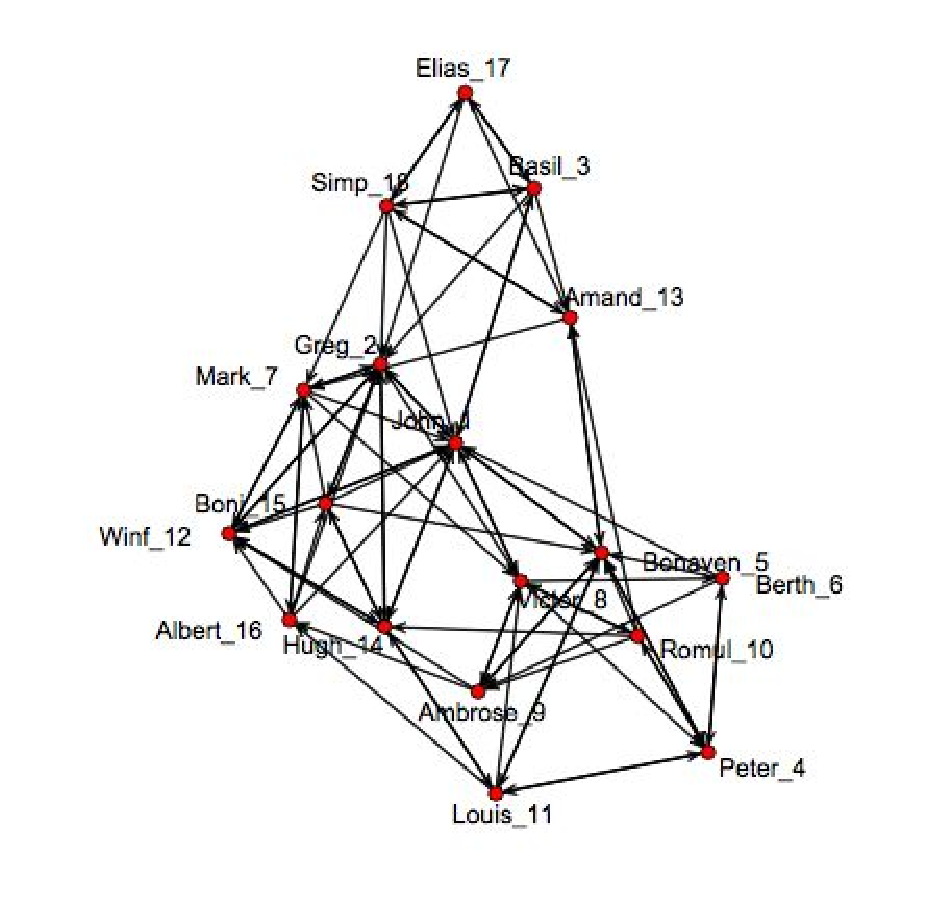
\includegraphics[width=5in, trim=0.2in 1in 0.3in .6in, clip=true ]{samplike} % l b r t
\end{center}
\caption[\citeauthor{Sampson}'s \citeyearpar{Sampson} monastery affinity network]
{\citeauthor{Sampson}'s \citeyearpar{Sampson} monastery affinity network.  \citeauthor{Sampson} collected data to define a ``liking" network among 18 monks 
in a New England monastery in the late 1960s.  Since ``liking" is a directional 
relation, the presence of a relation is depicted by an arrow rather than a line.  Data 
is available through and plotted using the \texttt{ergm} package \citep{ergm:R} in R.}
\label{F:Sampson}
\end{figure}

Stochastic network models were developed as early as 1959 in the seminal works of 
\citet{Gilbert} and \citet{Erdos}, resulting in a simple probabilistic model that is 
now referred to as the Bernoulli model or the Erd\"{o}s-R\'{e}nyi-Gilbert model.  Over 
the last forty years, more sophisticated stochastic network models have flourished;  
notable landmarks include the $p_1$ model of \citet{Holland:1981} which captures the 
reciprocal tendency of relationships in directed networks, and the $p^*$ model of 
\citet{Frank:1986} which describes the transitive tendency of relationships in 
undirected networks.  These models laid the foundation for the more general 
\emph{exponential random graph models (ERGM)}, a class of exponential family 
models that are now routinely used to model network data and are presented in 
detail in Section~\ref{S:ERGM examples}.\footnote{To be precise, they should
be called ``exponential \emph{family} random graph models", but apparently
this is too cumbersome.} 
% \citep{logit,Pattison:1999,Handcock:2006,introp*,advancesp*,recentp*,ergm,Morris:
%2008,Goodreau:2009,Goldenberg:2009}.

%\subsection{THE ISSUE -- DEPENDENCE}
At their core, stochastic network models attempt to describe whether or not a tie 
forms between each pair of actors in a group.
%  In the Florentine marriage network depicted in Figure~\ref{Padgett}, a model fit  
It has long been observed that relations, especially those involving humans, do not 
form in isolation; rather, they form in an interdependent manner.  Whether or not a 
relation forms between individuals $A$ and $B$ may very well depend on whether or not 
relations form between $B$ and $C$ and $C$ and $A$.  This has profound implications 
for the social scientist, necessitating a new ``network" perspective that recognizes 
the relational structures, such as a triangle of relations between actors $A$, $B$, 
and $C$, as factors in the analysis \citep[Chapter 1]{Wasserman:1994}.  This perspective has 
garnered increasing attention across different social and behavioral science 
disciplines over the last forty years, as evidenced by the rapid growth in publication 
of social network related papers \citep[Chapter 1]{Knoke:2008}.
% in the social science literature 
  
For the statistician, the network perspective means that the model should not break the 
network down into independent components, each containing two actors.
Instead, a good model will consider important relational structures in the observed network 
and clarify their contribution in shaping the global outcome.   
Accompanying the model must also be a computational algorithm to calibrate the model 
parameters to the network data.  
%In fact, this is the focus of our research.
In fact, writing down the expression for an uncalibrated ERGM turns out to be quite
straightforward; it is fitting the model
to data that is an open research problem and the focus of this dissertation.

Typically, parameter estimation for statistical models is done through the method of 
\emph{maximum likelihood} in which values for the parameters called \emph{maximum 
likelihood estimators (MLE)} that index the model to make the observed data most likely 
are calculated.
Many methodologies have been developed over the years to address the difficulties
in this process for exponential families
including Besag's \emph{pseudolikelihood} approach \citep{Besag:1974,Strauss:1990}, 
\citeauthor{Geyer:1992}'s \citeyearpar{Geyer:1992}
\emph{Markov chain Monte Carlo Maximum Likelihood} (MCMC-ML) approach, and 
\emph{stochastic approximation}.\footnote{Stochastic approximation has more general
applications in root finding, but is frequently used for parameter estimation.}
In fact, it was the absence of usable methodologies in parameter estimation that 
restricted earlier models like $p_1$ and $p^*$ to their simpler modeling capabilities.

%the simple expression belies the difficulties involved in fitting the model to data.
%In this paper, we describe further advances to these methodologies that address some of the
%pathologies researchers have encountered with these approaches.

Once model parameters are properly estimated, the completed model can be used to simulate 
new random networks whose distribution retains essential characteristics of 
the observed network.  Researchers can then use this 
to test hypotheses about the process of relationship formation.  
In this dissertation, we consider the ability to do statistical inference 
as the end goal of parameter estimation rather than the parameter values 
themselves.  This requires obtaining the maximum likelihood \emph{distribution} which
can then be used to construct confidence intervals and evaluate hypotheses.

%Similarly, exponential random graph models have a deceptively simple form \eqref
%{E:ERGM} that belies the challenges involved in estimating the model parameters.  

%Network researchers have developed many descriptive statistics to capture 
%characteristics of a network.  For example, the number of ties going to a particular 
%actor is one measure of that actor's prestige in that network \citep{Wasserman:1994}.  

Finally, it should be noted that although problems from the social sciences provide much of the 
motivation for social network analysis and our research here, network models can in 
fact be applied to problems in a broad range of disciplines including political 
science, biology, epidemiology, and computer science and may be of interest
to business practitioners in the utility or transportation sectors.  
Actors often represent individuals but 
they may also represent entities like nation-states, protein molecules, airports, 
computers, or corporations.  The relation that connects actors 
is often friendship or actor $A$ 
``liking'' actor $B$, as in Sampson's monk data depicted in Figure~\ref{F:Sampson}, 
but the relation can be any kind, such as a business transaction or the 
Internet connectedness between computers.  Figure~\ref{F:ecoli} depicts the
\textit{Escherichia coli} gene transcription network among 423 mRNA molecules 
\citep*{Shen-Orr,Salgado}. This data was 
modeled with an ERGM by \citet*{Saul:2007} and again by \citet*{Hummel}.

\begin{figure}[h!]
\begin{center}
\includegraphics[width=5in, trim=0.2in 0.in 0.2in .in, clip=true ]{ecoli} % l b r t
\end{center}
\caption[\textit{E. coli} transcriptional regulation network of \citet{Shen-Orr}]{\textit{E. coli} transcriptional regulation network of \citet{Shen-Orr}.  Each node is an operon (a group of genes transcribed into a single mRNA molecule) and a directed edge from one node to another indicates 
that the first encodes the transcription factor that regulates the second.
Data is available through and plotted using the \texttt{ergm} package \citep{ergm:R} in R.}
\label{F:ecoli}
\end{figure}



%%%%%%%%%%%%%%%%%%%%%%%%%%%%%%%%%%%
\subsection{Why model networks?}
Before we step into a lengthy of discussion of how we model network data, it is 
worth reflecting upon the question of why network models are desirable or interesting.  We 
have already given one answer to this question in the context of the social scientist 
trying to differentiate between competing underlying forces that can shape the global 
structure of relationships: a network model will allow the researcher to 
identify if one or more actor specific variables and network structures 
contribute to the characteristic of the overall network.  That is, a good statistical 
model can see past noise in the data to
provide clarity of the underlying forces that shape the structure of an observed network
\citep*{Goodreau:2009}.   

In the context of epidemiology, a model for  
a \emph{contact network}, which is a network of the potential disease-causing ties between individuals, may be useful in understanding the general mechanism by which an epidemic can spread.  This may in turn help formulate an intervention strategy \citep*{Welch:2011}.
In computational biology, network models may be used to better understand the processes
by which proteins interact \citep*{Goldenberg:2009}.  
Some other applications of networks are the links between sites on the Internet
or the international relations between countries.  At its essence, 
a network is a conduit for flow, whether it be the flow of diseases, commodities, 
data, capital, or ideas, and network models can help us
 understand the mechanism of this flow \citep*{Kolaczyk:slides}.

\section{Exponential random graph models} \label{S:ERGM setup}
A network can be modeled as a random  $n \times n$ matrix $Y$, where $n$ is 
the number of actors.
Each entry $Y_{ij}$ in the random matrix $Y$ is itself a random variable representing 
a relation from actor $i$ to actor $j$, such that:
\[
	Y_{ij} = 
	\begin{cases}
		1 & \text{if a relation exists \textit{from} actor $i$ \textit{to} actor 
$j$ (notation: $i \to j$)}\\
		0 & \text{otherwise}
	\end{cases}
	\
\]
where $i$ and $j$ take values in $1, \ldots, n$, $i \neq j$.  
Note that $Y_{ij}$ take only values of $0$ or $1$, reflecting our restriction 
on networks to those with \emph{dichotomous} relations, that is, the relation between a pair 
of actors is either present or absent.  In addition, we do not allow  
$i \to i$ and always have $Y_{ii} = 0$.  In the special case that 
$Y_{ij} = Y_{ji}$ and thus the matrix $Y$ is symmetric, the network is referred to as an
\textit{undirected} network or graph, such as in the case of the Florentine marriage 
network depicted in Figure~\ref{F:Florentine}.  A network is \textit{directed} if it is 
not undirected, as in the case of monastery affinity network depicted in 
Figure~\ref{F:Sampson}.  

The exponential family random graph model (ERGM) commonly used in the network 
literature for $Y$ has probability mass function of the following form:
\begin{align}
	f_\eta(y) = P_{\eta}(Y=y) = \frac{1}{ \kappa( \eta) } e^{ \inner{ \eta, g(y)}  } \qquad y \in \YY, \label{E:ERGM}
\end{align}
where $g(y)$ is a $d$-vector of \emph{natural statistics}, $\eta$ is a 
$d$-vector of \emph{natural parameters}, 
$\inner{\fatdot,\fatdot}$ denotes the bilinear form
\begin{align*}
	\inner{ \eta, g } = \sum_{i=1}^d g_i \eta_i,
\end{align*}
and $\YY$ is the sample space of all possible networks with $n$ actors.
So that \eqref{E:ERGM} integrates to 1, $\kappa(\eta)$ is a normalizing constant such that
\begin{align}
   \kappa(\eta) &= \int e^{ \inner{ \eta, g(x)}  } \, d \mu(x) \label{E:kappa}
\end{align}
where $\mu$ is a measure on $\YY$.  In fact, \eqref{E:ERGM} is exactly the form of 
an exponential family distribution in \emph{canonical form} \citep[Chapter 1.4]{tpe}.  The only distinction that makes this an ERGM is that $\YY$ is specified to be the 
discrete state space of all possible network configurations.

We rely on many properties of exponential families.  Define 
the \emph{natural parameter space} $\Xi$ as the set of points
$\eta = (\eta_1, \ldots, \eta_d)$.
An exponential family is \emph{full} if the natural parameter  space is
\begin{align*} %\label{E:paramspace}
   \Xi &= \{ \eta \in \RR^d : \kappa(\eta) < \infty \},  
\end{align*}
 and \emph{regular} if, in addition, $\Xi$ is an open set.
%The exponential family is \emph{full} if the natural parameter space is \eqref
%{E:fullparam}, and \emph{regular} if, in 
%addition, $\Xi$ is an open set.  
We say an exponential family is \emph{minimal} if the natural parameter  and 
natural statistic are not each concentrated on a hyperplane. 
Minimality guarantees that if an MLE, denoted $\etaMLE$, exists, 
it is unique \citep{Geyer:gdor}.


Define the \emph{cumulant} function as $c(\eta) = \log \kappa(\eta)$ and
denote the observed data as $\yobs$.  We can then express 
the log likelihood of \eqref{E:ERGM} as
\begin{align}
	\ell( \eta ) = \inner{ \eta, g(\yobs)} - c( \eta). \label{E:loglike}
\end{align}

The appeal of exponential families in the setting of complex dependence phenomena such 
as networks stems from their simplicity and maximum entropy property 
\citep{Jaynes:1978,Geyer:1992}.
By choosing statistics of interest on the data, one fully specifies a model that,
from a maximum entropy perspective, gives the 
most reasonable inference possible  derived solely from those statistics.  
Furthermore, exponential families have been 
well-studied \citep{Barndorff,Brown:1986} and utilized over the decades and have 
desirable properties such as the MLE uniqueness noted above.

%%%%%%%%% NETWORK STATISTICS
Ideally then, a network researcher need only specify relational structures of 
interest to define an ERGM.  
\citet*{Wasserman:1996, Pattison:1999, logit, introp*} describe many of 
the classical network statistics that one might include in the natural statistic vector 
$g(y)$.  In these works, the researchers' primary 
consideration in defining a network statistic is a relational structure's 
scientific interpretability.  
For example, in a directed affinity network, a sociologist may be 
interested in the propensity for individuals to form \emph{reciprocal} relations, where 
ties exist $i \to j$ and $j \to i$, or \emph{transitive} relations, where 
ties exist $i \to j$, $j \to k$, $i \to k$.  The statistics vector $g(y)$ 
that captures these can be defined by
\begin{align*}
	g(y) = \left ( \sum_{i<j} y_{ij}y_{ji}, \sum_{i \neq j \neq k} y_{ij}y_{jk}y_{ik} 
			\right )  
\end{align*}
where its components count the number of reciprocal and transitive relational 
structures in the network $y$.  
Such a model, with parameters appropriately calibrated to the affinity network, 
should then generate networks that exhibit a frequency of reciprocal and 
transitive relations similar to that of the observed data.
We will not discuss the merits of all the different network statistics 
here; in fact, there is essentially an unlimited number of potential network statistics.
What is important is that these statistics can be transparently calculated for a 
given network and the inclusion of them in $g(y)$, paired with their parameter 
components in $\eta$, allows the model \eqref{E:ERGM} to calculate probabilities of 
different global network outcomes $y$.  \citet*{ergm:userterms} 
even provide an interface for one to
customize and create her own network statistic of interest and model it in the 
\texttt{ergm} package in R.

%%%%%% RECENT NETWORK STATISTICS
More recently, \citet*{Handcock:2006, Hunter:2006, recentp*} developed
new network statistics with particular emphasis on the properties of 
the distributions as opposed to 
the scientific interpretability of the statistics themselves.
It had repeatedly been discovered that for some fitted models, the random networks generated
 from them did not at all resemble the observed network.  These new statistics
are intended to reduce the occurrence of such cases.
 A fairly complete description of these more recent network 
statistics is in \citet*{Morris:2008}.  We make use of one of these network statistics
in the example in Section~\ref{S:Example:FauxMagnolia}.
%We return to this issue in more detail in Section~\ref{S:Non-existent MLE}.
%In addition, the issue of model selection between competing models has not been 
%addressed though \citet{GOF} have begun making strides in this area.  Both of these 
%areas are active area of research.



%%%%%%%%%%%%%%%%%%%%%%%%%%%%%%%%%%%
\subsection{Intractable normalizing constant} \label{S:intractable}
We now return to the issue of why parameter estimation for ERGMs and 
similar exponential family models on discrete state spaces can be challenging.
Despite the tremendous appeal of the exponential family framework, one 
immediate problem is that the summation in \eqref{E:kappa} for the 
normalizing constant $\kappa(\eta)$ is over all possible 
networks in the sample space $\YY$ and can be prohibitively expensive to 
evaluate for networks of even moderate size.
For an undirected network with $n$ actors, there are $2^{{n\choose 2} }$ 
different possible networks in $\YY$.  Table~\ref{T:number graphs} shows how rapidly this number grows; 
unless dealing with networks of 9 actors or less, the likelihood function 
should not be directly evaluated.  See Appendix~\ref{A:Triangle count}
for our approach for counting simple network statistics in the 9-node network
relying on numerous tricks in data representation and computation.

\begin{table}[h!] 
\caption{Sample space size for undirected networks with different number of 
actors.}

\begin{tabular}{ccl} 
\hline 
Nodes & Possible Edges & Total Graphs \\ [1ex]
\hline
5 & ${5 \choose 2} = 10$ & $2^{10} = 1024$ \\ [1ex]
6 & ${6 \choose 2} = 15$ & $2^{15} = 32,768$ \\ [1ex]
7 & ${7 \choose 2} = 21$ & $2^{21} = 2,097,152$ \\ [1ex]
8 & ${8 \choose 2} = 28$ & $2^{28} = 268,435,456$ \\ [1ex]
9 & ${9 \choose 2} = 36$ & $2^{36} = 68,719,476,736$ \\ [1ex]
10 & ${10 \choose 2} = 45$ & $2^{45} = 3.518437\times10^{13}$ \\ [1ex]
\hline 
\end{tabular} \label{T:number graphs}
\end{table}

%%%%%%%%%%%%%%%%%%%%%%%%%%%%%%%%%%%
\subsection{Covariate data} \label{S:Covariate}
Information about a particular actor, say gender, can be incorporated as 
covariate data into the model with little difficulty.
Often, a social scientist looks to include such information because she is interested in
whether or not there is an \emph{assortative mixing} effect, that is, whether individuals of the same ``type" tend to make more relations with others of that type \citep{Goodreau:2009}.  
Suppose we wish to incorporate $p$ such exogenous attributes for our $n$-actor network.  
This information can be represented by an $n \times n \times p$ matrix $X$, whose 
$ijk$th element is the value of the $k$th attribute in the potential relation from actor
$i$ to $j$ \citep*{Fienberg:1981,ergm}.  We include such factors in our model 
of an adolescent friendship data set in Section~\ref{S:Example:FauxMagnolia}.

Like the other network statistics discussed, the statistics that comprise $X$ can 
be transparently calculated from data and hence included in the canonical 
statistics vector as $g(y, X)$,
with the canonical parameter vector $\eta$ lengthened accordingly.
The parameter estimation methodology is unchanged from before (so long as $p$ is not
excessively large), and while this greatly expands the
usefulness of ERGMs to the researcher, there are no new issues for us to consider
from a statistical modeling perspective.
Thus we will continue to use $g(y)$ instead of $g(y,X)$ for simplicity.  



%%%%%%%%%%%%%%%%%%%%%%%%%%%%%%%%%%%
\section{Examples of ERGMs} \label{S:ERGM examples}
We now review the classical Erd\H{o}s-R\'{e}nyi-Gilbert, $p_1$, and $p^*$ models to give both a sense of commonly used network structures as well as parameter estimation methodologies.

\subsection{Erd\H{o}s-R\'{e}nyi-Gilbert model} \label{S:Erdos}
The simplest example of an exponential random graph is the Erd\H{o}s-R\'{e}nyi-Gilbert 
model \citep{Erdos,Gilbert}, also referred to as a Bernoulli network model, which 
assumes that each actor forms a relation to every other actor independently with the 
same probability $p$ \citep{ergm}.  The ERGM can be expressed as
\begin{align*}
	P_{\eta}(Y=y) &= \frac{1}{\kappa( \eta) }e^{\eta g(y)}  \qquad y \in \YY, 
\end{align*}
where the only network statistic is a count of the number of edges for the directed network
\begin{align*}
%	g(y) = \frac{1}{N}\sum_{i \neq j} y_{ij},
	g(y) = \sum_{i \neq j} y_{ij}
\end{align*}
and the probability of a tie formation between any pair of actors is the same,
\begin{align*}
	p = P_\eta( Y_{ij} = 1) = \frac{e^{\eta}}{1+e^{\eta}}.
\end{align*}
%and thus the $Y_{ij}$ are mutually independent of one another.  
Then the log likelihood can be expressed as
\begin{align*}
	\ell(\eta) = \eta \sum_{i \neq j} y_{ij} - n(n-1) \log (1+ e^\eta).
\end{align*}

The MLE of $\eta$, $\etaMLE$, can be found analytically to be the logit of the 
fraction of ties that are present in the observed data set, 
\begin{align*}
	\etaMLE = \logit \left ( \frac{\sum_{i \neq j} y_{\textrm{obs}, ij}}{ n(n-1) } \right )
\end{align*}
where $n(n-1)$ is the number of possible ties in a directed network with $n$ actors.  
The MLE 
for $\eta$ is thus easily calculated from the observed data. The independence 
assumption, however, is too unrealistic for all but the simplest of cases; usually, 
a researcher is interested in modeling different probabilities of tie formations 
between actors.  Thus the Erd\H{o}s-R\'{e}nyi-Gilbert model may be most 
useful as a ``null'' model, though it is arguably too simple even for this.

%%%%%%%%%%%%%%%%%%%%%%%%%%%%%%%%%%%
\subsection{The $p_1$ model} \label{S:p1}
\citet{Holland:1981} made advances in relaxing this independence assumption  with 
their $p_1$ model.  They focused on two empirical observations from sociometric 
studies:
\begin{itemize}
\item Reciprocation: there tend to be a ``surplus" of mutual relationships in network 
data sets compared to a uniform distribution of directed relationships.
\item Stars: some individuals attract a surplus of choices compared to a uniform 
distribution of directed relationships.
\end{itemize}
\citeauthor{Holland:1981} then constructed a family of distributions with parameters 
to control the probability of observing different numbers of mutual relationships and 
stars.  
Focusing on the \textit{dyad}, the set of a pair of actors and the possible relations 
between them, as the basic building block, they proposed the following model:
\[
	P( Y = y ) = \frac{1}{ K( \rho, \theta, \{ \alpha_i \}, \{\beta_j \} )}\exp \left 
\{  \rho m(y) + \theta y_{++} + \sum_i \alpha_i y_{i+} +  \sum_j \beta_j y_{+j}\right 
\}
\]
subject to $\sum_i \alpha_i = \sum_j \beta_j = 0$, where
\begin{align*}
	\rho &= \text{``force of reciprocation" or mutuality parameter}\\
	m(y) &= \sum_{i \neq j} y_{ij}y_{ji}, \quad \text{total number of mutual relationships 
in $y$}\\
	\theta &= \text{``density" or overall choice effect parameter}\\
	y_{++} &= \sum_{i \neq j} y_{ij}, \quad  \text{total number of relations in $y$}\\
	\alpha_i &= \text{``productivity" or ``expansiveness" effect parameter for node $i
$}\\
	y_{i+} &= \sum_{j} y_{ij}, \quad  \text{``out-degree" for node $i$ in $y$}\\
	\beta_j &= \text{``attractiveness" or ``popularity" effect parameter for node $j$} 
\\
	y_{+j} &= \sum_{i} y_{ij}, \quad  \text{``in-degree" for node $j$ in $y$}\\
	K &= \text{normalizing constant}
\end{align*}

By defining new dyad random variables, $D_{ij} = (Y_{ij}, Y_{ji} )$, \citeauthor
{Holland:1981}  showed that with some algebraic manipulation, the form of the model above 
can be viewed as a log-linear model with independent dyad random variables 
$D_{ij}$.  This makes it possible to use a standard logistic regression to calculate MLEs of the parameters.

The statistical independence at the dyad level, however, means that this model will 
not capture triangular tie configurations (or anything more complicated) in which dyads are dependent.  Also, to 
reduce the number of parameters, the model assumes $\rho_{ij} = \rho$ and $\theta_{ij} = \theta$, meaning that the 
tendency towards reciprocity and forming relations is assumed to be the same across all actors.  This example 
illustrates how the parameter estimation methodology limits the scope of the model and 
what types of behavior it can capture.  

%%%%%%%%%%%%%%%%%%%%%%%%%%%%%%%%%%%
\subsection{Markov graph model}
\citet{Frank:1986} relaxed the independence assumption further with the implementation 
of \textit{Markov dependence} in which two dyads are independent, conditional on the 
rest of the graph, when they do not share a node.  The model uses only three 
configurations in an undirected network, expressed as:
\[
	P( Y = y ) = \frac{1}{K( \theta, \sigma, \tau)}\exp 
				\left \{ \theta L + \sigma S + \tau T	\right \} 
	\]
where
\begin{align*}
	\theta &= \text{edge parameter} \\
	L &= \sum_{i < j} y_{ij}, \quad \text{total number of edges} \\
	\sigma &= \text{2-star parameter, propensity for individuals to have connections 
with two actors} \\
	S &= \sum_{i < j < k} y_{ij}y_{ik}, \quad \text{total number of 2-stars ($i \leftrightarrow j$, $i \leftrightarrow k$) }\\
	\tau	&= \text{Triangle parameter, represents clustering} \\
	T &= \sum_{i < j < k} y_{ij}y_{jk}y_{ik}, \quad \text{total number of triangles ($i \leftrightarrow j$, $j \leftrightarrow k$, $i 
\leftrightarrow k$)}
\end{align*}
None of the above parameters have subscript indices, reflecting the simplification 
from a \textit{homogeneity} assumption where parameters are equated if the 
network structures are the same ignoring the labels on the nodes (also called \textit
{isomorphic} configurations.  In fact, this is the same simplification \citeauthor{Holland:1981} employ for the $\rho$ and $\theta$ parameters in their $p_1$ model).

The model is the first to break dyad independence, made possible by \citeauthor{Frank:1986}' methods of parameter estimation.  In particular, \citeauthor{Frank:1986} ran
Markov chain Monte Carlo simulations of the model at multiple values for a parameter 
to determine which fit the data best.  The authors also obtained 
\emph{maximum pseudolikelihood estimators (MPLE)} from a standard logistic 
regression (we discuss the pseudolikelihood approach in Section~\ref{S:pseudolikelihood}) 
and observed that the MPLEs are close to those they arrived at from their rigorous simulations.   \citeauthor{Frank:1986} seem to conclude that MPLEs are generally quite acceptable.  


%%%%%%%%%%%%%%%%% SECTION %%%%%%%%%%%
\section{ERGM parameter estimation}
Exponential random graph models have a deceptively simple form \eqref
{E:ERGM} that belies the challenges involved in model parameter estimation.
As discussed in Section~\ref{S:intractable}, the difficulties
arise from a normalizing constant \eqref{E:kappa} which may involve 
a summation over an astronomical number of terms.
In this section, we discuss commonly used parameter estimation methods
used for exponential families with complex dependence like ERGMs.  All approaches avoid evaluating the likelihood function directly but have properties that we
find undesirable.   The methods are aided by a strictly concave 
log likelihood function (see Section~\ref{S:Expfam theory}).  Thus there is
no concern for local maxima, and the global maximum, if it exists, is unique.
  
%These provide the backdrop for the new algorithm we propose in this paper.

%However, even with increasingly sophisticated simulation methods, finding MLEs for 
%ERGMs can be problematic in two ways:
%\begin{enumerate}
%\item The methodology used to find MLEs fails due to a shortcoming in the methodology 
%itself.  That is, an alternative approach might yield parameter estimates resulting in 
%a perfectly good model.
%
%\item The model itself is specified in such a manner so that it can be classified as 
%\emph{degenerate}, a term first applied to ERGMs by \citet{Handcock:Degeneracy} and 
%further clarified by \citet{Rinaldo:2009} to refer to instances where
%\begin{enumerate}
%\item Random graphs generated from the fitted model lack variability, often only 
%giving rise to unrealistic graphs, usually empty or complete (or nearly complete).
%\item the MLE does not exist.
%\item The fitted model makes the observed network highly unlikely.
%\end{enumerate}
%\end{enumerate}
%The two issues are related; for example, if the MLE does not actually exist, then 
%commonly used algorithms sent to find it will surely fail, or worse, return values 
%that the user may then treat as correct.   The issue is significant enough to be a 
%barrier to the use of ERGMs \citep{advancesp*}.



\subsection{Maximum pseudolikelihood method} \label{S:pseudolikelihood}
As mentioned in Section~\ref{S:p1}, \citet{Frank:1986} successfully applied 
the maximum pseudolikelihood method to social network models, a method first used in lattice systems in plant biology \citep{Besag:1974,Besag:1975}.  \citet{Strauss:1990} further justified the use of 
maximum pseudolikelihood estimators (MPLE) as reasonable approximations for MLEs in 
social network models.  \citet*{Wasserman:1996, Pattison:1999, logit} leaned on this 
result to broaden the scope of network models, allowing 
for any combination of network structures to be considered.  The result is \eqref{E:ERGM},
the more general form of the ERGM that is currently used.

The method of maximum pseudolikelihood finds the values for the parameters that 
maximize the \textit{pseudolikelihood function} for the observed 
data set, which can be constructed from the densities of $Y_{ij}$ 
conditional on the rest of network, denoted by $f_{Y_{ij}}( y_{ij} \mid \textrm{rest})$.
The pseudolikelihood function $PL(\eta)$ is defined to be the product of these densities,
\begin{align}
	PL(\eta) = \prod_{i \neq j}f_{Y_{ij}}( y_{ij} \mid \textrm{rest}), \label{E:PL}
\end{align}
and in general is different than the likelihood function.

Define the vector of \textit{change statistics} $\delta_g(y)_{ij}$ to be
\begin{align*}
	\delta_g(y)_{ij} = g(y_{ij}^+) - g(y_{ij}^-)
\end{align*}
where $y_{ij}^+$ and $y_{ij}^-$ represent networks with $y_{ij} = 1$ and $y_{ij} = 0$, 
respectively, while leaving the rest of the network as $y$.  Thus $\delta_g(y)_{ij}$ 
is the change in $g(y)$ when $y_{ij}$ changes from 0 to 1.
The conditional distribution of $Y_{ij} \mid \textrm{rest}$ for an ERGM is then a Bernoulli 
distribution with log odds
\begin{align}
	\log \left ( \frac{P( Y_{ij} =1 \mid \textrm{rest} ) }
				 	 { P( Y_{ij} =0 \mid \textrm{rest} ) } \right ) 
					 			= \eta^T \delta_g(y)_{ij}. \label{E:logodds}
\end{align}
%(See \citet*[Appendix]{Composite} for a derivation of \eqref{E:logodds}.)  
The form of \eqref{E:logodds} in the context of \eqref{E:PL} naturally lends
itself to the use of logistic regression to find values of $\eta$ that
maximize $PL(\eta)$.  These values of $\eta$ are called the maximum pseudolikelihood estimators.

In the case where $Y_{ij}$ are in fact mutually independent, the MPLEs will equal the MLEs.  
\citet{Strauss:1990} show that in 
many cases with dyad dependence, MPLE still yield reasonable approximations of the 
true MLEs.  

However, \citet*{Geyer:1992, Snijders:2002, introp*, Duijn:2009} demonstrated that 
the pseudolikelihood approach can produce very misleading results 
when dependence is strong.  
\citet*{Composite} showed that the pseudolikelihood approach can be 
improved upon in a generalization 
called the \emph{composite likelihood} approach; this method is identical
to pseudolikelihood except that the conditional distributions used to build the \emph{composite likelihood function}---analogous to the pseudolikelihood function \eqref{E:PL}---are for multiple 
ties rather than a single tie.
%Nevertheless, researchers now avoid citing parameter estimates based on these approaches.
\citet{Hummel} raised two additional issues with the pseudolikelihood approach, 
which also apply to the composite likelihood approach. 
The first is that this approach requires
an actual network $\yobs$ from which to derive the MPLE, as opposed to a network
statistics $g(\yobs)$ which may be some vector of theoretical interest to 
which one would like to fit an ERGM.  Thus given a $g(\yobs)$, one would then
need to take the extra step of finding a $\yobs$ that matches this vector of
interest.  The second point is that there are several networks that
yield the same $g(\yobs)$.  Because ERGMs depend only on $g(\yobs)$ and not $\yobs$,
these will all yield the same MLE.  However, there is no guarantee that they will yield the same MPLE.
Network software packages such as \texttt{statnet} \citep*{statnet:R} in the R 
platform now overwhelmingly use MLE methods, using MPLEs only as starting points
as in the example in Section~\ref{S:Example:FauxMagnolia}.

%%%%%%%%%%%%%%%%%%%%%%%%%%%%%%%%%%%%%%%%%%%%%%%%%
\subsection{Newton-Raphson}
Newton-Raphson is one of the most commonly used root-finding algorithms
in optimization, attractive
for its speed of convergence.  It relies on iterated updates of a root 
function, which in our setting is the gradient of the log likelihood, $\nabla \ell(\eta)$.  
The algorithm also requires the Hessian matrix $\nabla^2 \ell(\eta)$ and has updates 
of the following form:
\begin{align}
	\eta_{k+1} = \eta_k - \left[ \nabla^2 \ell(\eta_k) \right ]^{-1} \nabla \ell(\eta_k).
\end{align}
The algorithm may fail to 
converge when the initial $\eta_k$ is far from the solution.  However,
when Newton-Raphson does converge, it converges extremely fast, 
where the number of accurate digits roughly doubles at each step.

We use a stochastic version of Newton-Raphson in Section~\ref{S:Example:Ising} where 
we wish to calculate MLEs for comparison purposes and are able to start the algorithm from the known true parameter value.
Both $\nabla \ell(\eta)$ and $\nabla^2 \ell(\eta)$ can be approximated using MCMC 
 \citep{Penttinen:1984}.
%%%%%%%%%%%%%%%%%%%%%%%%%%%%%%%%%%%%%%%%%%%%%%%%%
\subsection{Markov chain Monte Carlo maximum likelihood} \label{S:MCMC-MLE}
\citet{Geyer:1992, Corander:1998, Snijders:2002} developed Markov chain Monte Carlo 
(MCMC) methods to approximate the MLE of an exponential family.  Of these, \citeauthor
{Geyer:1992}'s Markov chain Monte Carlo-maximum likelihood estimator (MCMC-MLE) method 
appears to have become the standard approach in the network literature 
\citep{Hunter:2006, Handcock:2006, GOF} and is the default algorithm in 
the \texttt{statnet} suite \citep{statnet:R} in the R platform for network models.  

The MCMC-MLE approach is theoretically guaranteed to converge to the MLE if it exists.  
Rather than maximizing the log likelihood \eqref{E:loglike}
with respect to $\eta$, \citeauthor{Geyer:1992} consider 
the log of the likelihood ratio $r( \eta, \eta^0 )$, where $\eta^0$ 
is fixed at a known value,
\begin{align}
 r( \eta, \eta^0 ) &= \ell( \eta ) - \ell( \eta^0 ) \notag \\ 
				  &= \inner{ \eta - \eta^0, g(\yobs)} - \log \left [ \exp \bigl( c(\eta) - c(\eta^0) \bigr) \right ].\label{E:r}
\end{align}
The value of $\eta$ that maximizes an
approximation of $r( \eta, \eta^0 )$ is then a good estimate of the MLE, 
assuming it exists.  In order to avoid evaluating the problematic normalizing constant,
this approach equates the ratio of normalizing constants 
$\exp \left (  c(\eta) - c(\eta^0) \right )$ to an expectation 
using \eqref{E:kappa} as follows:
\begin{align*}
	\exp \left (  c(\eta) - c(\eta^0) \right ) &= \frac{ \int \exp \bigl ( \inner{ \eta, g(x) }\bigr ) \, d\mu(x) }{ \kappa(\eta^0)  } \\
	&= \frac{ \int \exp \left ( \inner{ \eta - \eta^0, g(x)} + \inner{ \eta^0, g(x)} \right ) \, d\mu(x)  }{ \kappa(\eta^0) } \\
	&= \int \exp \left( \inner{\eta - \eta^0, g(x} \right ) \frac{ e^ { \inner{ \eta^0, g(x)} } }{ \kappa(\eta^0) } \, d\mu(x)\\
	&= \E_{\eta^0} \exp \left( \inner{ \eta - \eta^0, g(Y)}  \right ) .
\end{align*}
It should be noted that while we choose $\eta_0$ to index a distribution from the same
family as the one indexed by $\eta$ in \eqref{E:r}, in fact its distribution need 
only have the same support.
We will continue with this restriction not only for simplicity but also because this is how
the methodology is implemented for ERGM parameter estimation in the \texttt{statnet} package
\citep{ergm:R} in R.

By the Markov chain strong law of large numbers (or Birkhoff ergodic theorem), this 
expectation can be approximated by the sample mean for large Monte Carlo sample 
size,
\begin{align*}
	\frac{1}{m} \sum_{i=1}^{m}\exp \left ( \inner{ \eta - \eta^0,g(Y_i)} \right )
\end{align*}
where $Y_1, \ldots, Y_m$ are draws from the exponential family distribution with 
parameter $\eta^0$.  This sample can be generated using MCMC 
methods such as Metropolis-Hastings (used for ERGMs) or Swendsen-Wang (used for the Ising model example in Section~\ref{S:Example:Ising}); 
see 
\citet[Chapter 1]{Brooks} and references cited therein.

Thus \eqref{E:r} can be approximated by
\begin{align}
\hat{r}_m( \eta, \eta^0 ) &= \inner{ \eta - \eta^0, g(\yobs)} - \log 
	\left [ \frac{1}{m} \sum_{i=1}^{m} \exp \left ( \inner{ \eta - \eta^0, g(Y_i)} \right ) \right ] 
%	\left [ \frac{1}{m} \sum_{i=1}^{m} e^{  \inner{ \eta - \eta^0, g(Y_i)} } \right ] 
	\label{E:r_hat}
\end{align}
and for any fixed $\eta$
\begin{align*}
	\hat{r}_m( \eta, \eta^0 ) \to r( \eta, \eta^0 ) \text{ a.s. as $m \to \infty$}.
\end{align*}
This holds for all $\eta$ in any countable set and thus for some dense set.
If we call $\hat{\eta}_m$  the maximizer of \eqref{E:r_hat} and assume that the MLE 
$\etaMLE$ exists, \citeauthor{Geyer:1992} show that 
\begin{align*}
	\hat{\eta}_m \to \etaMLE, \quad \text{a.s.}
\end{align*}
 whenever the Markov chain is ergodic. 
 
This approach has been shown in practice to be sensitive to initial parameter 
values when used without the trust region methodology recommended in \citet{Geyer:1992}, 
and the algorithm may require enormous---sometimes infeasibly large---Monte Carlo sample sizes 
when the starting value $\eta^0$ is far from the MLE \citep{ergm}.  
In addition, \citeauthor{Geyer:1992} recommend iterating the algorithm several times, 
where each successive maximizing value will be closer to $\etaMLE$ than the previous \hl{GALIN: HOW DO WE KNOW THIS?}.  At the 
time of this writing, the MCMC-MLE routine in \texttt{statnet} uses by default 10,000 
Monte Carlo samples spaced 100 samples apart and a maximum of three iterations, using the 
MPLE as the initial value for $\eta^0$ \citep{statnet:R}.  
Improvement of the MCMC-MLE approach is an active area of research \citep*{Bartz}.
An extension of this method by \citet{Hummel} is discussed in the next section.

\citet{ergm} illustrate the practical difficulty associated with a poor initial 
value in the MCMC-MLE algorithm with Sampson's monastery data set depicted in 
Figure \ref{F:Sampson}.  The 
observed network $\yobs$ is directed with 18 actors and 88 ties present out of $18 \cdot 17=306$ possible 
ties.  To illustrate the issue, \citeauthor{ergm} use the Erd\H{o}s-R\'{e}nyi-Gilbert model 
described in Section~\ref{S:Erdos} with network statistic $g(y)$ equal to the total number of 
edges present.  As noted earlier, the true MLE is equal to 
\begin{align*}
	\etaMLE = \logit\left( \frac{g(\yobs)}{n(n-1)}\right) = \logit \left( \frac{88}{306}\right ) = -0.9072.
\end{align*}
  
When $\eta^0$ is chosen to be $1$, however, \citeauthor{ergm} show that it is
extremely difficult for the algorithm to attain the MLE in a single iteration of 
the MCMC-MLE algorithm.  
For this value of $\eta$, the model dictates that each of the 306 possible edges occur independently with probability $p = \frac{1}{1+e^{-\eta}} = \frac{1}{1+e^{-1}} = 0.731$.   
This is a very high probability relative to the sparsity of relations in the observed data 
set, which suggest a much smaller probability of tie formation of $88/306= 0.288$.  
In fact, the probability of obtaining fewer than 88 ties for the $\eta=1$ model is nearly zero at $2.3 \times 10^{-59}$, calculated using a binomial distribution with $n=306$, $p =0.731$.  

\begin{figure}[h!]  
\begin{center} 
%{\includegraphics[width=2.95in]{mcmc-mle1}}
%{\includegraphics[width=2.95in]{mcmc-mle-1}}
{\includegraphics[width=3.2in]{mcmc-mle1-bw}}
{\includegraphics[width=3.2in]{mcmc-mle-1-bw}}
\end{center} 
\caption[Log likelihood ratio approximations for Sampson's monastery data set]{Log likelihood ratio approximations for Sampson's monastery data set.  Top: $\eta^0 = 1$, Bottom: $\eta^0 = -1$. Solid lines are exact log likelihood ratios $\ell(\eta) - \ell(\eta^0)$, dotted lines are the 
approximation by \eqref{E:r_hat} using 100,000 MCMC samples.  
MLE is at $-0.9072$.
Data for plots are produced using code accompanying \citet{Hummel}.} 
\label{F:MCMC-MLE}
\end{figure} 

The MCMC-MLE algorithm maximizes the approximated log 
likelihood ratio \eqref{E:r_hat}.  However, the first derivative of $\hat{r}(\eta,\eta^0)$ with respect
to $\eta$ shows that if the MCMC sampler is unable to generate any $g(Y)< g(\yobs)$, 
the derivative of 
\eqref{E:r_hat} will be strictly negative, resulting in $\hat{r}(\eta,\eta^0)$ with no
maximum.  This is depicted by the dotted-line in Figure \ref{F:MCMC-MLE} (top).  
The problem is not present when the initial value is close to the true MLE, such as 
when $\eta^0 = -1$; the corresponding $r(\eta,\eta^0)$ and $\hat{r}(\eta,\eta^0)$ 
functions are depicted in Figure \ref{F:MCMC-MLE} (bottom).  With the default three 
iterations of MCMC-MLE in the \texttt{statnet} package, the algorithm 
starting with $\eta^0 = 1$ is only able to obtain an estimate for $\eta$ as 
small as $\eta = -0.364$.  With 10 iterations, it does in fact 
arrive at the MLE of $-0.907$.

\hl{GALIN: what about interval estimates}

%%%%%%%%%%%%%%%%%%%%%%%%%%%%%%%%%%%%%%%%%%%%%%%%% 
\subsection{Steplength MCMC-MLE} \label{S:Hummel}
\citet{Hummel} expanded the range for which iterated MCMC-MLE will converge by
making incremental updates in $\eta$ towards $\etaMLE$ possible at each iteration.  
As noted in the 
previous example with 
Sampson's monastery data, $\hat{r}(\eta,\eta^0)$ 
will have no maximum if $g(\yobs)$ is outside the range of MCMC samples.  
\citeauthor{Hummel}'s approach involves 
replacing $g(\yobs)$ with a value $\hat{\xi}_1$ close to $g(\yobs)$ but within
the range of the current model's MCMC samples.
This makes it possible to maximize $\hat{r}(\eta,\eta^0)$ and update $\eta^0$,
with the resulting $\eta$ necessarily closer to $\etaMLE$.

The approach is effective for Sampson's monastery example discussed, and was also applied
to the \emph{E. coli} biological network data of \citet{Shen-Orr} when 
starting from the MPLE.  Care is needed in finding a $\hat{\xi}_1$ that is inside
the range of the current model. In addition, if $\eta_0$ is very far from $\etaMLE$, it is 
not clear that the steps taken by this approach will be large enough to traverse
the distance between $\eta^0$ and $\etaMLE$ in any reasonable amount of time.



%\subsection{Generalization to exponential families}
%
%The algorithm and approaches we present here are generally applicable to all regular 
%exponential families on finite state spaces, including ERGMs.  Thus we present the 
%background theory at the higher level of exponential families though we will return to 
%ERGMs in our most complicated applications.

    
%%%%%%%%%%%%%%%%%%%%%%%%%%%%%%%%%%%%%%%%%%%%%%%%%
\subsection{Stochastic approximation}

Variations on the Robbins-Monro \emph{stochastic approximation} (SA) algorithm 
\citep{Robbins-Monro} have been applied to find the MLE similar contexts: 
\citet{Younes:1988,Younes:1989,Moyeed:1991,Gu:2001}
applied MCMC stochastic approximation to spatial models and \citet{Snijders:2002} to 
ERGMs.
%Our approach shares a similar recursive mechanism with SA, so we will describe this 
%method further.  
SA procedures for finding the MLE of a parameter $\eta$ generate iterated estimates 
$\eta_k$ to find the 
root of a gradient function $h(\eta)$:
\begin{align} \label{E:eta SA update}
	\eta_{k+1} = \eta_k + \alpha_k U_k,
\end{align}
where $\alpha_k$ is a step size and is typically a member of a decreasing sequence of 
positive numbers, and $U_k$ is a 
random variable from the distribution specified by $\eta_k$ that noisily estimates the 
gradient function $h(\eta_k)$.  

Restrictive conditions are required of $\alpha_k$ and $U_k$ to establish convergence 
of the sequence $\eta_k$.  
In Robbins-Monro SA \citep{Robbins-Monro}, the step size $\alpha_k$ must be a sequence 
of positive constants 
that satisfies 
\begin{align*}
	\sum \alpha_k^2 < \infty
%	\sum \alpha_k = \infty, \qquad \sum \alpha_k^2 < \infty.
\end{align*}
for which the choice of
\begin{align} \label{E:SA step size}
	\alpha_k = \frac{A}{B + k}
\end{align}
 is commonly used, where $A$ and $B$ are constants that must be specified by the user.  
This specification requires experimentation and care: there can be significant 
variation in performance depending on choice of these constants. 
A large body of more recent research \hl{presents support} for a sequence that goes to 0 
more slowly than $1/k$ 
for faster convergence \citep[Chapter 11]{Kushner:1997}, but still requires 
experimentation.  
%Regardless of the exact form, there is no guarantee the likelihood function will 
%increase at each update. 

The conditions on $U_k$ are more restrictive.  Popular approaches include constraining 
the sequence of estimators $\eta_k$ to a compact set specified \emph{a priori}, 
or assuming that the noise component of $U_k$ be a martingale 
difference sequence.  As commonly observed \citep*{Chen:2002,Andrieu:2005,Liang:2010} 
these may be 
difficult to satisfy in practice.  
See \citet{Andrieu:2005,Liang:2010} for recent developments that impose less 
restrictive conditions using truncated 
updates.

An issue for any recursive search algorithm is the 
choice of starting point.  It is 
often the case that algorithms are good at finding the MLE when the starting point is 
close to it, but of course the 
location of the MLE is unknown.  For any exponential family with bounded support, 
Fisher information 
becomes singular as the canonical parameter $\eta$ goes to $\infty$ \citep*{Rinaldo:2009}.
Hence methods which rely on 
the Fisher information matrix may fail when the starting point for $\eta$ is far from 
the MLE \citep{Younes:1989,Gu:2001}.
Of course, one may try different starting points until a ``good'' one is found, but 
this comes with no theoretical guarantees and can be cumbersome in practice.

%%%%%%%%%%%%%%%%%%%%%%%%%%%%%%%%%%%%%%%%%%%%%%%%%
\subsection{Summary of parameter estimation methods}
Tables~\ref{T:Compare estimation} and \ref{T:Compare MCMCestimation} summarize the advantages and disadvantages of the exact and MCMC parameter estimations discussed.  
All methods assume that the MLE exists before the search algorithm is applied and that
the log likelihood is strictly concave.

\begin{table}[h!] 
\caption[Comparison of exact parameter estimation methods]{Comparison of exact parameter estimation methods. MPLE=Maximum pseudolikelihood estimator, Newton=Newton-Raphson,
SA=stochastic approximation.\\}

\begin{tabular}{|c|l|l|}
\hline 
Method & Appeal & Drawbacks \\ [1ex]
\hline
\multirow{2}{0.5in}{MPLE}		
& 	\textbullet \, Simplicity 				  	& \textbullet \, \hl{Maximizes} $PL(\eta)$, not $\ell(\eta)$  \\
& 	\textbullet \, Speed, via logistic regression 	& \\ [1ex] % \textbullet \, MPLE behavior not well understood \\ [1ex]
\hline
\multirow{3}{0.5in}{Newton}
& 	\textbullet \, Converges rapidly when it & \textbullet \, Requires second derivative matrix and its\\	
%& \textbullet \, Highly sensitive to starting point\\ 
& 	converges 	&  \\ [1ex] 
\hline
\multirow{3}{0.5in}{SA} 		
& 	\textbullet \, Simple updates 				& \textbullet \, Requires trial-and-error calibration  \\			& 	\textbullet \, Theoretically guaranteed to		& \textbullet \, Highly sensitive to starting point \\
& 	converge to MLE with proper  & \textbullet \,  May converge too slowly to be practical \\
& 	setup  & \\[1ex]
\hline 
\end{tabular} 
\label{T:Compare estimation}
\end{table}

\begin{table}[h!] 
\caption[Comparison of MCMC parameter estimation methods]{Comparison of MCMC parameter estimation methods. MCMC Newton=MCMC Newton-Raphson,
MCMC-MLE=Markov chain Monte Carlo-maximum likelihood estimator, 
step MCMC-MLE=steplength MCMC-MLE,
MCMC SA=stochastic approximation.\\}

\begin{tabular}{|c|l|l|}
\hline 
Method & Appeal & Drawbacks \\ [1ex]
\hline
\multirow{4}{0.5in}{MCMC Newton}
& 	\textbullet \, Converges rapidly when it  & \textbullet \, Requires calculation of second derivative \\
& 	converges 	& matrix (computationally expensive) \\				
&				& and its inverse (positive defniteness) \\[1ex]
\hline
\multirow{3}{0.5in}{MCMC-MLE}
& 	\textbullet \, Theoretically guaranteed to   	& \textbullet \, Highly sensitive to starting point \\ 
& 	converge to MLE 					& \textbullet \, May require enormous MC sample sizes\\ 
&				& \textbullet \, May require several iterations\\ [1ex]
\hline
\multirow{3}{0.5in}{step MCMC-MLE}
& 	\textbullet \, Theoretically guaranteed to   	& \textbullet \, Sensitive to starting point \\ 
& 	converge to MLE 					& \textbullet \, Requires setup expertise\\ 
& \textbullet \, Increased range 		& \textbullet \, May require several iterations\\ [1ex]
\hline
\multirow{3}{0.5in}{MCMC SA} 		
& 	\textbullet \, Simple updates & \textbullet \, Requires trial-and-error calibration  \\			
& 	\textbullet \, Theoretically guaranteed to	 & \textbullet \, Convergence conditions not easily\\
& 	converge to MLE, though & implemented in practice.\\
& 	under restrictive conditions.  & \\ [1ex]
\hline 
\end{tabular} 
\label{T:Compare MCMCestimation}
\end{table}
%%%%%%

%\begin{figure}[h]
%\begin{center}
%\includegraphics[width=4.5in]{mck.pdf}
%\end{center}
%\caption{What I got out of case studies.}
%\label{F:mck}
%\end{figure}

%%%%%%%%%%%%%%%%%%%%%%%%%%%%%%%%%%%%%%%
\section{Non-existent MLEs in exponential families} \label{S:Non-existent MLE}
Parameter estimation via maximum likelihood for exponential family models with 
complex dependence---already a 
challenging problem because the likelihood function may be computationally 
infeasible---is further obfuscated by the possibility that the MLE
may not exist.  
In such a case, the strictly concave likelihood function is
increasing in some direction of the parameter space, called a 
\emph{direction of recession}, so that the MLE is actually off ``at infinity".
The theoretical background 
for this situation has been understood for many years 
\citep{Barndorff,Brown:1986}: MLE existence is a
geometric problem relating to properties of the \emph{convex support} of the model,
which is  the smallest closed convex set 
that the contains the natural statistic \citep{Geyer:gdor}.  
The MLE does not exist in the conventional sense if the 
observed data is on the relative boundary of this 
convex support (see Section~\ref{S:MLE existence}).
When this occurs, 
it may exist in the \emph{Barndorff-Nielsen completion} of the family.
Before this dissertation, there have been no 
computationally convenient approaches to handling this issue for social network models
and other discrete exponential family models with complex dependence.

\citet{Geyer:1992} separated the search for the MLE of an exponential family model
with complex dependence into a two-phase algorithm, 
where phase I determines whether or not an MLE exists in the conventional 
sense via linear programming, and phase II finds the MLE when it exists.
\citeauthor{Geyer:1992}'s MCMC-MLE method discussed in Section~\ref{S:MCMC-MLE} corresponds to phase II of
this approach.
In the special case of generalized linear models including logistic regression and contingency 
tables, \citet{Geyer:gdor} outlines a methodology to detect non-existent MLEs and construct 
one-sided confidence intervals for the natural parameters.
The approach applies linear programming to the polyhedral convex support of 
the model to determine the \emph{face} of the convex support 
on which the observed data lies.  
This face in turn defines the convex support for a new exponential family for which the MLE 
does exist and can be found using conventional methods (see Section~\ref{S:LCM}).
The linear programming 
functionality has been implemented in the R package \texttt{rcdd} \citep*{rcdd:R}.

\citet*{Handcock:degeneracy, Rinaldo:2009} focus on problematic instances of parameter 
estimation for ERGMs, which are loosely referred 
to as \emph{degeneracy}.  Strictly speaking, a distribution in an exponential
family is degenerate when it concentrates the distribution of the natural statistic
on a hyperplane.  If the family is minimal, this occurs if and only if the MLE does not exist in the conventional sense.  This in turn means that the observed
data lies on the relative boundary of the convex support.  \emph{Near} degenerate  
means that the observed data lies nearly on this relative boundary.
However, the terms degeneracy and nearly degeneracy
are now invoked if there are undesirable behaviors of the fitted model or 
in the model fitting process itself
\citep{Handcock:degeneracy,advancesp*,recentp*,statnet-tutorial}.
We will only use the terms for their original meanings here.   

\begin{figure}[h!]
\centering
\includegraphics[width=5in]{Figures/g9-hull-bw}
\caption[Sample space of two-dimensional statistic for 9-node network model]{Sample space 
of two-dimensional statistic for 9-node network model.  \citet{Rinaldo:2009} focused
on edge and triangle statistics.  The shading of a point corresponds to 
the frequency of graphs with that network statistic.  
The convex support is the gray, sail-shaped polytope.  Points on the 
boundary have an outlined circle and extreme points are square.}
\label{F:g9-hull}
\end{figure}

To better understand ERGM pathologies, \citeauthor{Handcock:degeneracy,Rinaldo:2009}
study small networks with 7 and 9 nodes.  At these sizes, it is still 
possible to explicitly evaluate the likelihood function \eqref{E:ERGM} and thus 
find MLEs using standard numerical optimization routines.  
As in \citep{Geyer:gdor}, the emphasis is on the geometric properties of the 
polyhedral convex support of the model;
the convex support for the 9-node ERGM with a two-dimensional network statistic of
edges and triangles
studied by \citeauthor{Rinaldo:2009} is depicted in Figure~\ref{F:g9-hull}.
\citeauthor{Rinaldo:2009} showed that the normal cones (see Section~\ref{S:Convex analysis}) of this support
explain which portions of the natural parameter space are more likely to correspond to 
degenerate and nearly degenerate models.  Some of the perceived pathologies then, 
are fully explained by exponential family theory and are not pathologies at all.

However, it is possible for a well-fit model to poorly describe or resemble the 
observed data \citep{Handcock:degeneracy,ergm}.  This may include cases of multimodality of 
the distribution of the natural statistic and extreme sensitivity to parameter
values.  %This has been observed and studied in Ising models \citep{Potts}. 
In the multimodality case, the observed data is the average
of the distribution, but there are multiple modes, none which resemble the observed
data.  If the distribution is in addition extremely sensitive to parameter values,
it is possible for a very small change in the parameter value to lead to a 
very different distribution, perhaps going from multimodal to unimodal.
When these behaviors are too problematic, the model itself
should be changed.  ERGMs give tremendous
flexibility in model specification but with no guarantees that a model will behave exactly as desired.  \citet*{GOF} devise graphical tests for evaluating the goodness of fit of ERGMs.
Their tools, available in the \texttt{statnet} package, compare characteristics of 
the distribution of networks simulated from the fitted model to the observed data, 
which can then be utilized to help choose between network statistics to include in a 
model. The issues described here are not with the parameter estimation method 
itself and thus are not the focus of this dissertation.  

%\citet{Okabayashi:longrange} present a ``long range" search algorithm to climb the log 
%likelihood of an exponential family, intended for settings where the initial guess of 
%the parameter value may be far from the MLE.  The algorithm is guaranteed to converge 
%when the MLE exists in the conventional sense.

%%%%%%%%%%%%%%%%%%%%%%%%%%%%%%%%%%%%%%%%%%%%%%%%%
\section{Research overview} \label{S:Research overview}
In this dissertation, we propose a simple and practical line search algorithm which
accomplishes the following objectives:
\begin{enumerate}
\item The algorithm converges to the MLE of any regular exponential family 
when the MLE exists.  It does so while
\begin{enumerate}
	\item avoiding the hassle of trial-and-error in algorithm calibration
	\item being insensitive to starting point and can thus be started from ``long range".
\end{enumerate}
\item When the MLE does not exist, the algorithm finds the MLE in the Barndorff-Nielsen completion and the 
accompanying direction of recession necessary to construct one-sided 
confidence intervals in the manner of \citet{Geyer:gdor}.
\end{enumerate}

In short, our proposed algorithm, outlined in the next section,
 addresses many of the drawbacks of the methods
described in Section~\ref{S:ERGM examples} as well as providing a general methodology
for dealing with non-existent MLEs.  We are not aware of any other 
general approaches for handling non-existent MLEs for ERGMs.  

We prove convergence for our algorithm in the case where the MLE exists and the first 
derivative of the log likelihood can be calculated exactly.
When the first derivative cannot be calculated exactly, 
it has a particularly convenient form that is 
easily estimable with MCMC, making the algorithm still useful in application.

The appeal of this algorithm is its usability: no trial and error is needed.  
Experimentation with multiple starting points or tuning parameters is not necessary 
and no unrealistic \emph{a priori} information about the problem need be specified.  
It is currently used in the \texttt{aster2} contributed R package 
\citep{aster:R} as the safeguard for steepest ascent and Newton-Raphson
 iterations in finding the MLE for aster models.

Our algorithm utilizes first derivative information only, evaluating 
neither the likelihood function itself nor derivatives of higher order than first.
The desire to avoid calculation of higher order derivatives in our algorithm
is motivated not just by 
computational considerations, but 
also by how much useful information can be extracted from them.   
%As noted previously, 
If the current value for $\eta$ is far from the MLE,  
the Fisher information matrix may be near-singular and algorithms like (unsafeguarded) 
Newton-Raphson algorithm may fail.  
For this 
reason, the best use of our algorithm may be from ``long range,'' filling a gap in the MLE estimation toolbox.  It may 
be expedient to switch to another algorithm like Newton-Raphson or MCMC-MLE 
after significant progress is made and the Fisher information matrix becomes useful.  

In the case where the MLE does not exist in the conventional sense, 
it is actually ``at infinity" in some direction of the parameter space.
Our algorithm returns the information necessary to construct one-sided confidence 
intervals for how close $\eta$ is to infinity.  
Previous work in this area with ERGMs utilized full knowledge
of the convex support \citep{Handcock:degeneracy,Rinaldo:2009}, something
not generally available for ERGMs, and provided no such confidence intervals.

%In \citet{Handcock:degeneracy,Rinaldo:2009}, the authors 
%authors work with small networks for which they have full knowledge of 
%the convex support, as in the case of the 9-node network depicted in Figure~\ref{F:g9-hull}.  While the authors dissect the various scenarios on these small networks
%in great detail, they recommend no general methodology 
%or tools to detect nor cope with non-exist MLEs in other networks.  
%Thus although we visit the same 9-node network example, we do so using a general 
%methodology that assumes no knowledge of the convex support \emph{a priori} and 
%outline a methodology that is generally applicable.


%%%%%%%%%%%%%%%%%%%%%%%%%%%%%%%%%%%%%%%%%%%%%%%%%
\subsection{Long range search algorithm overview}  \label{S:algorithm overview}

Our algorithm generates iterated estimates $\eta_k$ of the MLE with the 
update 
\begin{align} \label{E:eta update}
	\eta_{k+1} = \eta_k + \alpha_k p_k
\end{align}
where $\alpha_k$ is a \emph{step size} and $p_k$ is a \emph{search direction} and is 
restricted to be an ascent direction of 
the log likelihood.  
Despite the visual similarity between \eqref{E:eta SA update} and \eqref{E:eta 
update}, the line search approach treats 
the search direction $p_k$ in \eqref{E:eta update} as constant whereas in SA the 
corresponding $U_k$ in \eqref{E:eta SA update} is random.
Furthermore, line search algorithms have more restrictions on the step size $\alpha_k$.  
The step size 
conditions in the classical gradient ascent algorithm, which is the basis for our 
algorithm, force  a sufficiently 
large increase in the objective function at every step, guaranteeing convergence to 
the global maximum, if it exists.
%By contrast, there may be steps in SA that result in a decrease of the objective 
%function.   

Theorem 3.2 in \citet{NW} implies the global convergence of the steepest ascent 
algorithm for a continuously differentiable function, $\ell(\eta)$.  It requires the 
step length $\alpha_k$ to satisfy 
the Wolfe conditions for \emph{sufficient increase} and \emph{curvature}:
\begin{equation} \label{eq:wolfe}
\begin{split}
	\ell(\eta_k + \alpha_k \eta_k) \geq \ell(\eta_k) + c_1 \alpha_k \nabla \ell (\eta_k)^T p_k \\
	\nabla \ell( \eta_k + \alpha_k p_k)^T p_k \leq c_2 \nabla \ell( \eta_k)^T p_k
\end{split}
\end{equation}
where $\nabla$ is the gradient operator and $0 < c_1 < c_2 < 1$.   
Variations of these conditions exist in the numerical optimization \hl{literature} \citep
{Fletcher,NW,Sun:2006}, but all 
require evaluating the objective function.

Exponential families we consider are an unusual case in optimization in that the 
objective function 
is harder to compute than its derivatives and hence not previously considered by 
optimization theorists.
In our algorithm, we replace \eqref{eq:wolfe} with a single modified curvature 
condition:
\begin{align} \label{E:curvature mod}
	 0 & \leq \nabla \ell( \eta_k + \alpha_k p_k)^T p_k \leq c \nabla \ell(\eta_k)^T p_k
\end{align}
for some $0 < c < 1$.  This replacement is possible while still guaranteeing 
sufficient increase and convergence to the MLE (if it exists) 
because we have the additional property that the exponential family log likelihood 
function we consider is strictly 
concave.  The restrictions on the step size $\alpha_k$ along a particular direction 
$p_k$ are depicted in Figure~\ref{F:alpha_region}.  

\begin{figure}[h]
\centering
    \scalebox{.55}{\input{Figures/alphamax.pdf_t}}
	\caption[Acceptable region for step size $\alpha$ along search 
direction $p$ according to modified curvature condition]{Acceptable region for step size 
along a search direction according to modified curvature condition 
\eqref{E:curvature mod}. The step sizes $\alpha_{c}$ and $\alpha_{\textrm{max}}$ 
correspond to values of $\nabla \ell( \eta_k + \alpha p_k)^T p_k$ equaling 
$c \nabla \ell(\eta_k)^T p_k$ and $0$, 
respectively.  The condition ensures sufficient increase in the log likelihood along 
the search direction $p_k$.}
\label{F:alpha_region}
\end{figure}
 
 %%%%%%%%%%%%
%\hl{HMMMMM---WHERE TO PUT THIS PARAGRAPH.}  Our line search algorithm with $p_k$ 
%the Newton direction provides a
%safeguard for Newton-Raphson that makes it safe (not necessarily efficient) for use 
%from any range.
%%, though it is difficult to quantify what is significant progress since the 
%%limitations of these other algorithms are not well-defined.  
%The \texttt{aster2} contributed R package \citep{aster:R} switches $p_k$ from steepest 
%ascent direction to Newton direction
%after a fixed number of steps ($d / 2$ where $d$ is the dimension $\eta$) but always 
%finds a step length $\alpha_k$ satisfying
%\eqref{E:curvature mod}, iterating until the (unsafeguarded) Newton step satisfies 
%\eqref{E:curvature mod}.\\


%%% Can't just put a \newpage just anywhere in the text
%\pagebreak[3]

Our algorithm can be outlined as follows.  Let $\lVert \, \cdot \, \rVert$ denote the 
Euclidean norm function, and $\epsilon$ 
a small value greater than 0.  \\

% ALGORITHM 
\begin{singlespace} 
{
\noindent Get an initial value, $\eta_0$.\\ 
Set $k=0$. \\
Calculate $\nabla \ell( \eta_k)$, the direction of steepest ascent. \\
Set $p_k = \nabla \ell( \eta_k)$. \\
\textbf{while}  $\lVert \nabla \ell( \eta_k) \rVert > \epsilon$ \\ 
\hspace{4mm} \indent	 
\textbf{Find} a step size $\alpha_k$ that satisfies the modified 
curvature condition
\begin{align*}
	 0 & \leq \nabla \ell( \eta_k + \alpha_k p_k)^T p_k \leq c \nabla \ell(\eta_k)^T 
p_k
\end{align*}
\indent for some $0 < c < 1$.  
%This condition requires $\alpha_k$ to fall within \\
%\indent the acceptable region in Figure \ref{F:alpha_region}. \\


$\eta_{k+1} = \eta_k + \alpha_k p_k$.\\
\indent Calculate $\nabla \ell( \eta_{k+1})$.\\
\indent \textbf{Find} the new search direction $p_{k+1}$, which must be an ascent 
direction. \\
\indent $k = k + 1$.  \\
\textbf{end while}\\
}
\end{singlespace}
The exit condition from this algorithm is that $\lVert \nabla \ell( \eta_k) \rVert$
is close to zero.  As noted earlier, the log likelihood $\ell(\eta)$ is a strictly
concave function; when the global maximum $\etaMLE$ exists, $\lVert \nabla \ell( \etaMLE) \rVert = 0$.  
When the MLE does not exist in the conventional sense, $\ell(\eta)$ does not bend
 back down as depicted in Figure~\ref{F:alpha_region}, but instead continues to increase along some direction.  Hence the maximizer can be thought of as ``at infinity".
The log likelihood function is, however, still bounded by 
the log likelihood of 
the \emph{limiting conditional model}, which 
is another exponential family defined on a support for which the MLE is
guaranteed to exist, as discussed in Section~\ref{S:LCM}.
As part of the process to construct one-sided confidence intervals 
for how close $\eta$ is to infinity, 
our algorithm looks to find the maximizer for this new model.  
Some modification of this algorithm is necessary, which we discuss in 
Chapter~\ref{Chapter:Linear programming}.  In particular, the objective function
$\ell( \eta)$ that is being maximized must switch to that of the new model.
However, the overall structure of the algorithm is the same.

%DOES THE REST OF THIS CHAPTER NEED TO BE HERE AT ALL?  It is a well-known theorem of exponential families that the non-existence of the MLE 
%is synonymous with the the observed data occurring on a boundary of the 
%convex support $C$.
%Because we do not assume to know the full geometry of $C$, we do not know at the 
%outset if the MLE exists.  
%Thus we need to explore the sample space through sampling and determine on the fly 
%whether or not the observed data occurs on a boundary of the perceived 
%convex support.  
%Should this occur, the algorithm defines the limiting conditional model and 
%proceeds to maximize its log likelihood in search of the maximizer.
%
%\subsection{Examples in this paper??}
%
%% \section{Example: social network models} \label{S:Example}




%%%%%%%%%%%%%%%%%%%%%%%%%%%%%%%%%%%%%%%%%%%%%%%%%%%%%%%%
\chapter{Background Theory}\label{Section:Background}
%\input{Background}
All of the parameter estimation issues discussed thus far for ERGMs are relevant to 
the larger class of discrete state space exponential family models.
These models are commonly used to model phenomena with dependent structure, 
where the outcomes of the response variable of interest are in fact dependent on one 
another.  For example, the Ising 
model \citep{Ising,Potts} is an exponential family model that has been used to model 
ferromagnetism.  
%A realized 
%sample from this model is depicted in Figure~\ref{F:pottsimage}, where neighboring 
%pixels (representing atoms in a crystal lattice) are more likely to have the same 
%color.  
%We explore this model further in Section~\ref{S:Examples:Ising}.
Other examples of phenomena with dependent structure modeled with exponential 
families include
plant ecology \citep{Besag:1974,Besag:1975} and the lifetime fitness of plants \citep
{Shaw:2008}.

Although motivated by ERGMs, the algorithm we propose is rooted in fundamental
exponential family theory and applicable to any discrete state space 
exponential family model.  Thus the theory presented in this section is from
the perspective of exponential families in general.

\section{Exponential Family Theory}
An exponential family of distributions \citep{Barndorff,Geyer:gdor}
on a sample space $\YY$ has log likelihood \eqref{E:loglike}.
%\begin{align} 
%   \ell(\eta) = \inner{g(y), \eta} - c(\eta)
%\end{align}
%where $g(y)$ is a $d$-dimensional vector of canonical statistics, $\eta$ a $d$-
%dimensional vector of
%canonical parameters, and $\inner{\fatdot, \fatdot}$ denotes the bilinear form
%$$
%   \inner{g, \eta} = \sum_{i =1}^d g_i \eta_i.
%$$
%So that the probability function integrates to 1,
%the cumulant function $c$ must have the form
%\begin{align} \label{E:cumulant}
%      c(\eta) = \log \left(\int e^{\inner{g(y), \eta}} \, d\mu(y) \right),
%\end{align}
%where $\mu$ is a measure on $\YY$.
%Define
%\begin{align} \label{E:fullparam}
%	\Xi = \{ \eta \in \RR^q: c(\eta) < \infty \}.
%\end{align}
%The exponential family is \emph{full} if the natural parameter space is \eqref
%{E:fullparam}, and \emph{regular} if, in 
%addition, $\Xi$ is an open set.  We say an exponential family is \emph{minimal} if $g
%(y)$ is not concentrated on a 
%hyperplane. Minimality guarantees that if an MLE exists, it is unique \citep
%{Geyer:gdor}.

In finite state space models with complicated dependence like an Ising model or 
exponential random graph model,  \eqref
{E:cumulant} is a sum which may have no simple expression and can only be evaluated by 
explicitly doing the sum.
When the sample space $\YY$ is even moderately large, this can be prohibitively 
expensive.  For example, an Ising model 
defined on a $32\times 32$ square lattice where each entry takes values of 0 or 1, 
there are $2^{1024} \approx 10^
{300}$ elements in $\YY$.  A loop with this many iterations takes too long no matter 
how programmed.

A useful property of all exponential families \cite[p.~27]{TPE2} on which we rely 
heavily is that 
\begin{align*}
	\E_\eta(g(Y)) &= \nabla c(\eta)	\\
	\Var_\eta(g(Y)) &= \nabla^2 c( \eta ).
\end{align*}

Thus we can express first and second derivatives of the log likelihood \eqref
{E:loglike} and Fisher information, $I
(\eta)$, as
\begin{align}
	\nabla \ell( \eta ) &= g(y) - \E_\eta g(Y) \label{E:nabla ell} \\
	\nabla^2 \ell( \eta ) &=  - \Var_\eta g(Y) \label{E:nabla2 ell} \\
	\I(\eta) &= -\E_\eta \nabla^2 \ell (\eta ) = \Var_\eta g(Y) \label{E:FI}
\end{align}
and thereby avoid evaluation of the problematic cumulant function $c$.


By the strict convexity of the log likelihood function ensured by \eqref{E:nabla2 
ell}, the global 
maximum, if it is exists, is attained when $\eta$ is such that $\nabla \ell( \eta ) = 
0$, or, by \eqref{E:nabla ell},
\begin{align}
	\E_\eta g(Y) = g(\yobs). \label{E:Observed-Expected}
\end{align}


\section{Convex Analysis}
The issue of MLE existence in the conventional sense in an exponential family is 
closely tied to the geometric properties of 
the convex support of the model \citep{Barndorff, Geyer:gdor, Rinaldo:2009}.  We 
describe the relevant theory from convex analysis as it pertains to the case of 
exponential families.

A \emph{convex polytope} $C$ is the convex hull of a finite set of points $V$,
\begin{align*}
	C = \con( V ).
\end{align*}
where [\textbf{DEFINE pos().}]

  By the Minkowski-Weyl theorem \citep[Theorem 19.1]{Rockafellar:1970}, this convex 
set can equivalently be represented as the intersection of a finite collection of 
closed half-spaces.  These two representations of a convex polyhedron are referred to 
as the V-representation and H-representation, respectively.  
%The V-representation of a convex polyhedron $C$ is the set of all linear combinations
%\begin{align*}
%	\sum_{i \in E \cup I} b_i \alpha_i
%\end{align*}
%where $\alpha_i$ are vectors, $b_i$ are scalars, $E$ and $I$ are disjoint finite sets 
%such that
%\begin{align*}
%	b_i \geq 0, \quad i \in E \cup I
%\end{align*}
%and if $I$ is nonempty
%\begin{align*}
%	\sum_{i \in I} b_i = 1.
%\end{align*}

The H-representation can be expressed as the solution set of a finite set of linear 
equations and inequalities,
\begin{align*}
	C = \{x: Ax \leq b \},
\end{align*}
where $A$ is a matrix and $b$ a vector.

A nonempty \emph{face} of a convex polyhedron $C$ is a convex subset of $C$ such that 
every line segment in $C$ with a relative interior point in $F$ has both end points in 
$F$ \citep{Rockafellar:1970}.  It is itself a convex polyhedron.
A \emph{proper} face is a face that is not the empty set or $C$, and 
\emph{facets} are proper faces of the highest dimension.

The \emph{tangent cone} of a convex set $C$ at a point $x \in C$ is
\begin{align*}
	T_C(x) = \cl\{s(w-x):w \in C \text{ and } s \geq 0 \},
\end{align*}
where $\cl$ denotes the closure operation \citep[Theorem 6.9]{Rockafellar}.  

The \emph{normal cone} of a convex set $C$ in $\RR^d$ at a point $x \in C$ is 
\begin{align*}
	N_C(x) = \{ \delta \in \RR^d: \inner{w-x,\delta} \leq 0 \text{ for all } w \in C 
\}.
\end{align*}

Tangent and normal cones are polars of each other, that is, each determines the other.  
The normal cone at $x$ can be defined in terms of the tangent cone at $x$ by
\begin{align*}
	N_C(x) 	&= \{ w \in \RR^d: \inner{ w, v } \leq 0 \text{ for all } v \in T_C(x) \}.
\end{align*}

DEFINE \emph{direction of recession}, \emph{direction of constancy}.  \textbf{get from 
\citep{Rockafellar:1970}.}

\section{MLE existence in exponential families}
Charlie's GDOR theorems rely heavily upon some results from his thesis \citep{Geyer:
1990}.  Adapted here 
using the notation from his GDOR paper,
\begin{theorem}[Theorem 2.2 in \citep{Geyer:1990}]
\begin{align*}
e^{c(\theta + s \delta) - bs} &\to 
		\begin{cases} 
			0 								& b > \sigma_c(\delta) \\
			e^{c(\theta)} P_\theta(Y \in H ) 	& b = \sigma_c(\delta) \\
			+\infty							& b < \sigma_c(\delta)
		\end{cases}
& \text{as } s \to +\infty.
\end{align*}
where $\delta$ is a non-zero direction, $C$ the convex support, and
\begin{align*}
	\sigma_C (\delta) = \sup_{y \in C} \inner{ y, \delta} \\
	H_\delta = \set{w: \inner{w, \delta} = \sigma_C(\delta) }.
\end{align*}
\end{theorem}
$H_\delta$ is the supporting hyperplane to the set $C$ with normal vector $\delta$.

\begin{proof}
\textbf{Case: $b = \sigma_C(\delta)$.}

Starting with density of the exponential family with parameter $\theta$, we know that
\begin{align*}
	e^{c(\theta)} = \int h(y) e^{\inner{y,\theta}} \, dy.
\end{align*}
So,
\begin{align*}
	e^{ c(\theta + s \delta ) - bs } &= \int h(y) e^{\inner{y,\theta + s \delta - 
bs} } \, dy. \\
									&= \int h(y) e^{\inner{y,\theta}  + s [ \inner
{y,\delta} - b ] } \, dy. 
\end{align*}
Multiply by $\frac{p_\theta(y)}{p_\theta(y)}$ to get
\begin{align*}
	e^{ c(\theta + s \delta ) - bs } &= \int h(y) e^{\inner{y,\theta}  + s [ \inner
{y,\delta} - b ] }  \frac{ h(y)e^{\inner{y, \theta} - c(\theta)} }{ h(y)e^{\inner{y, 
\theta} - c(\theta)} }\, dy \\
	&= \int e^{  s [ \inner{y,\delta} - b ] + c(\theta) }  h(y)e^{\inner{y, \theta} - 
c(\theta)} \, dy \\
	&= \E_\theta e^{  s [ \inner{Y,\delta} - b ] + c(\theta) }
\end{align*}
What happens as $s \to +\infty$?  We would like to reverse the order of taking the 
limit and expectation.  Fortunately, we have the monotone convergence theorem.  For $
\inner{y, \delta} \leq b$, we have a monotonically decreasing sequence of random 
variables.  For $\inner{y, \delta} > b$, the sequence is increasing.  Thus,
\begin{align*}
	\lim_{s\to \infty} \E_\theta e^{  s [ \inner{Y,\delta} - b ] + c(\theta) } &= E_
\theta \lim_{s\to \infty} e^{  s [ \inner{Y,\delta} - b ] + c(\theta) }. 
\end{align*}
Ignoring the expectation and examining the just limit component of the above,
\begin{align*}
	\lim_{s\to \infty} e^{  s [ \inner{Y,\delta} - b ] + c(\theta) } &= 
			\begin{cases} 
			0 								& \inner{Y,\delta} < b \\
			e^{c(\theta)} 		 			& \inner{Y,\delta} = b \\
			+\infty							& \inner{Y,\delta} > b.
		\end{cases}
\end{align*}
In the case that we are considering, however, $b = \sigma_C(\delta) = \sup_{y \in C}
\inner{y,\delta}$, so $\inner{Y,\delta}$ can never be greater than $b$, so the third 
case in the limit above is not possible.  Thus we can rewrite the result above 
succinctly as
\begin{align*}
	\lim_{s\to \infty} e^{  s [ \inner{Y,\delta} - b ] + c(\theta) } &= I(\inner{Y,
\delta} = b ) e^{c(\theta)} 
	= I( Y \in H_\delta ) e^{c(\theta)}.
\end{align*}
Then returning to the full expression,
\begin{align*}
	\lim_{s\to \infty} \E_\theta e^{  s [ \inner{Y,\delta} - b ] + c(\theta) } &= e^
{c(\theta)} P( Y \in H_\delta ).
\end{align*}

\textbf{Case: $b > \sigma_C(\delta)$}.
\begin{align*}
	\lim_{s\to \infty} e^{ c(\theta + s \delta ) - bs } &= 
	\lim_{s\to \infty} e^{ c(\theta + s \delta ) - \sigma_C(\delta)s + \sigma_C
(\delta)s - bs }  \\
	&= \left( \lim_{s\to \infty} e^{ c(\theta + s \delta ) - \sigma_C(\delta)s} 
\right ) \left(  \lim_{s\to \infty} e^{ s[ \sigma_C(\delta) - b] } \right )\\
	&= \left (e^{c(\theta) }P(Y\in H_\delta) \right ) \cdot 0 = 0.
\end{align*}

\textbf{Case: $b < \sigma_C(\delta)$}.
\begin{align*}
	\lim_{s\to \infty} e^{ c(\theta + s \delta ) - bs } &= 
	\lim_{s\to \infty} e^{ c(\theta + s \delta ) - \sigma_C(\delta)s + \sigma_C
(\delta)s - bs }  \\
	&= \left( \lim_{s\to \infty} e^{ c(\theta + s \delta ) - \sigma_C(\delta)s} 
\right ) \left(  \lim_{s\to \infty} e^{ s[ \sigma_C(\delta) - b] } \right )\\
	&= \left (e^{c(\theta) }P(Y\in H_\delta) \right ) \cdot \left ( + \infty \right ) 
= + \infty.
\end{align*}
\end{proof}

The \emph{convex support} of an exponential family is the smallest closed convex set 
that the contains the natural statistic \citep{Geyer:gdor}.

\begin{theorem}[Theorem 1 from \citet{Geyer:gdor}] \label{Thm:DOC}
For a full exponential family with
\begin{itemize}
\item log likelihood function, $\ell(\eta)$, as in \eqref{E:loglike},
\item natural parameter space, $\Xi$, as in \eqref{E:fullparam},
\item natural statistic, $g(Y)$,
\item observed data, $\yobs$, such that $g(\yobs) \in C$, the convex 
support,
\end{itemize}
the following are equivalent:
\begin{enumerate}
\item $\delta$ is a direction of constancy of the log likelihood.
\item For all $\eta \in \Xi$, the function $s \mapsto \ell( \eta + s\delta)$ is 
constant on $\RR$ \cite[Theorem 1 (b)]{Geyer:gdor}.
\item The parameter values $\eta$ and  $\eta + s\delta$ correspond to the same 
probability distribution for all $\eta \in \Xi$ and all real $s$ \cite[Theorem 1 (d)]
{Geyer:gdor}.
\item $\inner{g(Y) - g(\yobs),\delta} = 0$ almost surely for all distributions in the 
family \cite[Theorem 1 (f)]{Geyer:gdor}.
\item $\delta \in N_C(g(\yobs))$ and $-\delta \in N_C(g(\yobs))$ \cite[Theorem 1 (g)]
{Geyer:gdor}.
\item $\inner{w,\delta} = 0$ for all $w \in T_C(g(\yobs))$ \cite[Theorem 1 (h)]
{Geyer:gdor}.
\end{enumerate}
\end{theorem}
The set of all directions of constancy is called the \emph{constancy space} of the log 
likelihood.

\begin{theorem}[DOR: Theorem 3 from \cite{Geyer:gdor}] \label{Thm:DOR}
For a full exponential family with the same setting as Theorem~\ref{Thm:DOC},
%\begin{itemize}
%\item log likelihood function, $\ell(\eta)$, described by \eqref{E:loglike},
%\item natural parameter space, $\Xi$,
%\item natural statistic, $g(Y)$,
%\item observed value of the natural statistic, $g(\yobs)$, such that $g(\yobs) \in C$, the convex 
%support,
%\end{itemize}
the following are equivalent:
\begin{enumerate}
\item $\delta$ is a direction of recession of the log likelihood.
\item For all $\eta \in \Xi$, the function $s \mapsto \ell( \eta + s\delta)$ is 
nondecreasing on $\RR$ \cite[Theorem 3 (b)]{Geyer:gdor}.
\item $\inner{g(Y) - g(\yobs),\delta} \leq 0$ almost surely for all distributions in 
the family. \cite[Theorem 3 (d)]{Geyer:gdor}.
\item $\delta \in N_C(g(\yobs))$ \cite[Theorem 3 (e)]{Geyer:gdor}.
\item $\inner{w,\delta} \leq 0$ for all $w \in T_C(g(\yobs))$ \cite[Theorem 3 (f)]
{Geyer:gdor}.
\end{enumerate}
\end{theorem}


%%%%%%%%%%%%%%%%%%%%%%% 1/26/11 - Added from Algorithm.tex
\subsection{Theorem 3(a) and (c), \citet[p. 270]{Geyer:gdor}}
So what do we this theorem for?  It relates when $\delta$ is a direction of recession 
or not.  Theorem 3 in GDOR has says the following are equivalent:
\begin{itemize}
\item (a) There exists a $\theta \in \Theta$ such that the function $s \mapsto \ell
(\theta+s\delta)$ is nondecreasing on $\RR$.
\item (c) $\inner{Y-y, \delta} \leq 0$ almost surely for all distributions in the 
family.
\end{itemize}

The $\delta$ in (a) in the above is a direction of recession.  

The proof requires the following lemma, which a PROOF WILL BE NEEDED.
$\ell(\theta+s\delta)$ is non-dereasing if and only if $\lim_{s \to \infty} \ell
(\theta+s\delta) > -\infty$.

\textbf{From $(c) \to (a)$}:

Take $\E_{\theta + s \delta}()$ of $\inner{Y-y, \delta} \leq 0$.  Then
\begin{align*}
\inner{ \E_{\theta + s \delta} Y-y, \delta} \leq 0.
\end{align*}
Now, take the derivative of $\ell( \theta + s\delta)$ with respect to $s$.
\begin{align*}
\deriv{\ell( \theta + s \delta}{s}) &= \deriv{}{s} \left (   \inner{y, \theta+s
\delta} - c(\theta+s\delta)  \right )\\
	&= \inner{y, \delta} - \deriv{}{s} c(\theta+s\delta) \\
	&= \inner{y, \delta} - \inner{ \E_{\theta+s\delta}Y,\delta }\\
	&= - \inner{ \E_{\theta+s\delta}Y - y,\delta }.
\end{align*}
Applying the above from the assumption, we get that 
\begin{align*}
\deriv{\ell( \theta + s \delta)}{s} \geq 0.
\end{align*}
Thus $\ell(\theta+s\delta)$ is a non-decreasing function of $s$.

\textbf{From $(a) \to (c)$}:
\begin{align*}
	\ell( \theta+s\delta) &= \inner{y, \theta+s\delta} - c(\theta+s\delta) \\
	&= \inner{y, \theta} + s \inner{y,\delta} -bs +bs - c(\theta+s\delta) \\
	&= \inner{y, \theta} + s [\inner{y,\delta} -b]  - \log e^{c(\theta+s\delta) -bs}.
\end{align*}
We know from the above lemma that $\ell(\theta+s\delta)$ is non-dereasing if and only 
if $\lim_{s \to \infty} \ell(\theta+s\delta) > -\infty$.  This implies that in the 
above expression, for the right-most term, $b \geq \sigma_c(\delta)$, and also that
\begin{align*}
	\inner{y, \delta} - b \geq 0,
\end{align*}
or 
\begin{align*}
	b - \inner{y, \delta}  \leq 0.
\end{align*}
If the above is true, then 
\begin{align*}
	\sigma_C(\delta)  - \inner{y, \delta} \leq b - \inner{y, \delta}  \leq 0,
%#	\inner{y, \delta} - \inner{Y_{max},\delta } \geq 0.
\end{align*}
and recalling that $\sigma_C(\delta) = \sup_{y \in C} \inner{y, \delta}$, then
\begin{align*}
	\inner{Y - y,\delta } \leq 0.
\end{align*}
(with probability one---do I even need to add this).
%%%%%%%%%%%%%%%%%%%%%%%%%%%%%%%%%

From the two theorems above, it is clear that every direction of constancy is a 
direction of recession.  These induce the following criteria about the existence of 
the MLE in the conventional sense:

\begin{corollary}[Theorem 4, Corollary 5 \citep{Geyer:gdor}] \label{Cor:MLE DNE}
For a full exponential family with the setting as Theorem~\ref{Thm:DOC}, if $\delta$ 
is a 
direction of recession that is not a direction of constancy, then  
\begin{enumerate}
\item the MLE does not exist.
\item $N_C(g(\yobs))$ is a vector subspace.
\item $T_C(g(\yobs))$ is a vector subspace.
\item for all $\eta \in \Xi$, the function $s \mapsto \ell(\eta + s \delta)$ is 
strictly increasing on 
the interval where it is finite.
\end{enumerate}
\end{corollary}

The \emph{relative interior} of a convex set $C$, denoted $\rint C$, is the interior 
relative to its affine hull.  We call $\delta$ a \emph{generic direction of recession} 
(GDOR) if $\delta \in \rint N_C(g(\yobs))$.  By construction it is not a direction of 
constancy.  By Corollary~\ref{Cor:MLE DNE}, a GDOR exists if and only if the MLE does 
not exist.

The well-known condition for the existence of the MLE \citep{Barndorff, Brown:1986} is 
formally stated as follows:
\begin{theorem} \label{Thm:MLE rint}
Under the conditions [CONDITIONS], the MLE exists in the conventional sense and is 
unique if and only if 
$g(\yobs) \in \rint(C)$.
\end{theorem}

When the MLE does not exist for an exponential family in the conventional sense, there 
exists a GDOR along which the log likelihood goes to $+\infty$.  The behavior of the 
density of the distribution is described in the following theorem:

\begin{theorem}[Theorem 6 from \citet{Geyer:gdor}] \label{Thm:LCM}
For a full exponential family with the setting as Theorem~\ref{Thm:DOC}, and 
additionally,
\begin{enumerate}
\item density function \eqref{E:pdf},
\item direction of recession, $\delta$,
\item $H = \{ w \in \RR^d: \inner{ w-g(\yobs), \delta } = 0 \}$,
\item $P( g(Y) \in H) > 0$ for some distribution in the family,
\end{enumerate}
then for all $\eta \in \Xi$
\begin{align} \label{E:LCM}
\lim_{s \to \infty} f_{\eta+s\delta}(y) = 
			\begin{cases} 
			0 								& \inner{g(Y) - g(\yobs), \delta} < 0 \\
			\frac{f_\eta(y)}{P_\eta(g(Y) \in H)} 	& \inner{g(Y) - g(\yobs),
\delta} = 0 \\
			+\infty							& \inner{g(Y) - g(\yobs), \delta} > 0.
		\end{cases}
\end{align}
If $\delta$ is not a direction of constancy, then $s \mapsto P_{\eta+s\delta}( g(Y) 
\in H)$ is continuous and strictly increasing, and 
$P_{\eta+s\delta}( g(Y) \in H) \to 
1$ as $s \to \infty$.
\end{theorem}


The right-hand side of \eqref{E:LCM} can be viewed as a conditional density of a 
distribution with parameter $\eta$ given $g(Y) \in H$ and hence expressed as $f_{\eta}
(\, \cdot\,  | g(Y) \in H)$ (the set that maps to $+\infty$ has probability zero by 
Theorem~\ref{Thm:DOR}).  Because it still has the same functional form as the 
exponential family density, $f_\eta(y)$, the family of distributions
\begin{align} \label{E:f conditional}
\{ f_{\eta}(\, \cdot\,  | g(Y) \in H) \text{ for } \eta \in \Xi \}
\end{align}
is itself an exponential family with the same natural parameters and statistics as the 
original family.  
%Then we can succinctly summarize the result of Theorem~\ref{Thm:LCM} as
%\begin{align*}
%\lim_{s \to \infty} f_{\eta+s\delta}(y) = f_{\eta}( y | g(Y) \in H).
%\end{align*}
It may not be full, however; the full family containing this exponential family,
\begin{align*}
\{ f_{\eta}(\, \cdot\,  | g(Y) \in H) \text{ for }  \eta + \gamma: \eta \in \Xi \text
{ and } \gamma \in \Gammalim \},
\end{align*}
where $\Gammalim$ is the constancy space of \eqref{E:f conditional},
is called the \emph{limiting conditional model} (LCM) \citep{Geyer:gdor}.  
An MLE for this new model must exist, since $g(\yobs)$ cannot lie on the boundary of 
the convex support which was itself determined by $g(\yobs)$ lying in the interior of 
it.  


\subsection{Theorem 6, \citet[p. 271]{Geyer:gdor}, 7/25/10}
And now the big one:
\begin{theorem}
If $\delta$ is a direction of recession, and
\begin{align*}
H = \set{ w \in \RR^p: \inner{w-y,\delta}=0 },
\end{align*}
and $P(Y \in H) > 0$ for some distribution in the family, and hence for all, then for 
all $\theta \in \Theta$,
\begin{align*}
\lim_{s \to \infty} f_{\theta+s\delta}(\omega) = 
			\begin{cases} 
			0 								& \inner{Y(\omega) - y ,\delta} < 0 \\
			\frac{f_\theta(\omega)}{P_\theta(Y \in H)} 	& \inner{Y(\omega) - y ,
\delta} = 0 \\
			+\infty							& \inner{Y(\omega) - y ,\delta} > 0.
		\end{cases}
\end{align*}
If $\delta$ is not a direction of constancy, then $s \mapsto P_{\theta+s\delta}( Y 
\in H)$ is continuous and strictly increasing, and $P_{\theta+s\delta}( Y \in H) \to 
1$ as $s \to \infty$.
\end{theorem}
Before going on to the proof, let's think about what this means.  Suppose $\delta$ is 
a DOR and not a DOC, because the latter is not interesting.  So, the MLE does not 
exist because the log-likelihood, despite being strictly convex, is strictly 
increasing when we go in the direction of $\delta$.  That's what DOR means.  So then 
what?

Well, we need to think first about $H$ again, this plane that is perpendicular to $
\delta$ on which the observed data $y$ lies.  Looking first at the last sentence of 
this theorem, it says that for the sequence of exponential families with parameter 
value $\theta+s\delta$, the probability of $Y$ occurring on the plane $H$ is strictly 
increasing, and in fact, going to 1.  This is what Charlie is referring to when he 
says things like ``the probability is accumulating on the boundary".  So, $H$ 
actually coincides with the boundary of the convex hull, the observed data $y$ sits 
is on this boundary (hence the MLE does not exist, by the usual MLE existence 
theorem, and hence a DOR exists).  When we take the parameter value further and 
further along in the direction of the DOR, the samples generated from that model will 
be increasingly cluster around that boundary face of the convex hull on which $y$ 
sits.

So how about the rest of the theorem?  We saw in Theorem 3 that $\inner{Y-y,\delta} 
\leq 0$ so the set where the above is $+\infty$ has probability zero.  I think the 
set for which $\inner{Y-y,\delta} = 0$ corresponds to a DOC, doesn't it?  Hmm, 
something's not right with my reasoning.

Charlie's paper says: the right side (excluding the 0 probability part) is the 
density of the conditional distribution given the event $Y \in H$ of the distribution 
having parameter value $\theta$, so we could denote the RHS by $f_\theta(\omega | Y 
\in H)$.  The exponential family with the \emph{full} natural parameter space (I'm 
glossing over some stuff) is the limiting condition model (LCM).  ``If an MLE exists 
for the LCM, then it maximizes the likelihood in the family that is the union of the 
LCM and the original family, and it maximizes the likelihood in the family that is 
the set of all limits of sequences of distributions in the original family.  When 
this happens, we say we have found an MLE in the Barndorff-Nielsen completion of the 
original family."

\begin{proof}
Hmm, I'm concerned about the different forms of $H$: are they actually all the same 
thing?  Well, carry on.

By Theorem 3, if $\delta$ is a DOR, then $\inner{Y-y, \delta} \leq 0$ which implies 
that $\inner{Y, \delta} \leq \inner{y, \delta}$.  So, the largest value that $\inner
{Y, \delta}$ can take on is $\inner{y, \delta}$.  Then $\sigma_C(\delta) = \inner{y, 
\delta}$.

Focus on the form of the density for $f_{\theta+s\delta}(\omega)$.  According the 
form of the relative density previously defined with respect to $\psi$,
\begin{align*}
 f_{\theta+s\delta}(\omega) &= e^{ \inner{y,\theta+s\delta - \psi} - c(\theta+s
\delta) + c(\psi)  } \\
 	&= e^{ \inner{y,\theta - \psi} -c(\theta) + c(\theta) + s \inner{y,\delta} - c
(\theta+s\delta) + c(\psi)  } \\
 	&= e^{ \inner{y,\theta - \psi} -c(\theta) + c(\psi) - c(\theta+s\delta) + s 
\inner{y,\delta} + c(\theta)   } \\
 	&= f_\theta(\omega) \frac{e^{c(\theta)}}{e^{ c(\theta+s\delta) - \inner{y,\delta}
s } }.
\end{align*}
This form is starting to look familiar, in particular, the denominator is from 
Theorem 2.2 from \citet{Geyer:1990} except with $\inner{y,\delta}$ instead of $b$ 
(where this 
$y$ is the dummy variable in the density, not the observed data).  So what happens as 
$s \to \infty$?  

It depends on how $\inner{Y(\omega),\delta}$ relates to $\sup_{y \in C}\inner{y,
\delta} = \inner{y,\delta}$, for the observed data $y$.  (our notation is getting a 
little confusing since $y$ can denote the observed data $y$ or the dummy variable in 
the density).  
\begin{align*}
	f_{\theta+s\delta}(\omega) = f_\theta(\omega) \frac{e^{c(\theta)}}{e^{ c(\theta+s
\delta) - \inner{y,\delta}s } } 
	\to	
			\begin{cases} 
			0 								& \inner{Y(\omega),\delta} < \inner{y,
\delta} \\
			\frac{f_\theta(\omega)}{P_\theta(Y \in H)} 	& \inner{Y(\omega) ,
\delta} = \inner{y,\delta} \\
			+\infty							& \inner{Y(\omega),\delta} > \inner{y,
\delta}.
	\end{cases}
\end{align*}
For $\delta$ a DOR but not DOC, we need to show that the $P_{\theta+s\delta}(Y \in H) 
\to 1$ 
as $s \to \infty$, where $H = \set{w \in \RR^p: \inner{w-\yobs,d}=0}$.
\begin{align*}
 P_{\theta+s\delta}(Y \in H) &= \int_H e^{\inner{y, \theta+s\delta - \psi} - c(\theta
+s\delta) + c(\psi)} \, d\psi \\
		&= \E_\psi \left \{ I_H e^{\inner{y, \theta - \psi} +c(\psi) - [c(\theta+s
\delta) -s\inner{y,\delta}]} \right 
\}\\
		&= \E_\psi \left \{ I_H  \frac{e^{c(\theta)} }{ e^{ c(\theta+s\delta) -s\inner
{y,\delta} } } 
		e^{\inner{y, \theta - \psi} -c(\theta)+c(\psi)}  \right \}.
\end{align*}
Since the indicator function, $I_H$, fixes $\inner{ y, \delta}$ to be a constant, it 
can pulled out of the expectation, so that 
\begin{align*}
		 P_{\theta+s\delta}(Y \in H)
		 &= \frac{e^{c(\theta)} }{ e^{ c(\theta+s\delta) -s\inner{y,\delta} } }
		 \E_\psi \left \{ I_H   
		e^{\inner{y, \theta - \psi} -c(\theta)+c(\psi)}  \right \}, \\
		 &= \frac{e^{c(\theta)} }{ e^{ c(\theta+s\delta) -s\inner{y,\delta} } } 
		 P_\theta ( Y \in H ).
		 \end{align*}
 
Then applying Theorem 2.2 from Geyer:1990,
\begin{align*}
 P_{\theta+s\delta}(Y \in H)
		&\to \frac{1}{P_\theta(Y \in H)}  P_{\theta}(Y \in H) = 1
 \end{align*}
 as $s \to \infty$.  
 
 That this probability is strictly increasing follows directly from the DOR property 
which requires $\ell( \theta+s
\delta)$ to be strictly increasing.   
\end{proof}


\subsection{log likelihood is bounded by LCM}
\subsection{summary}



In summary, by Theorem~\ref{Thm:MLE rint}, when the observed statistic, $g(\yobs)$, is 
on the boundary of the convex support $C$, the MLE does not exist in the conventional 
sense.
Then by Corollary~\ref{Cor:MLE DNE}, there must exist a direction of recession, $
\delta$, that is not a direction of constancy.  
According to Theorem~\ref{Thm:LCM}, as we move in the natural parameter space in the 
direction of $\delta$, the distribution with this parameter value will put 
increasingly probability on points for which the natural statistics, $g(Y)$, land in 
the hyperplane $H$ on which $g(\yobs)$ lies.  This hyperplane is orthogonal to $\delta
$ by construction and contains the boundary of the convex support.  Samples generated 
from these models will therefore increasingly fall on the face on which $g(\yobs)$ 
lies as $\eta$ increases in the direction of $\delta$.  Theorem~\ref{Thm:LCM} says 
that eventually, all generated sample points will fall on this boundary.


\subsection{Mean value parameterization}

An alternative parameterization of an exponential family is the mean value 
parameterization.  For each natural parameter $\eta$, we can define the mean parameter 
$\mu$ such that
\begin{align*}
	\mu = \E_\eta g(Y).
\end{align*}
The space for the mean value parameterization is the same as the convex support of the 
natural statistics and thus lends itself to easier interpretability  \citep
{Handcock:degeneracy, Rinaldo:2009}.  In particular, $\mu = g(\yobs)$ is the MLE in 
the mean value parameterization.  \citeauthor{Handcock:degeneracy} observed that mean 
value parameters located too close to the boundary of the convex support correspond to 
degenerate distributions.  

There exists a one-to-one mapping between a natural parameter and its mean value 
parameter, and one can calculate mean value parameters from natural parameters. In 
general there is no simply way to get the natural parameter value from the mean value 
parameter (if there was, then finding MLEs would be very easy and we wouldn't need all 
these algorithms!).

%%%%%%%%%%%%%%%%%%%%%%%%%%%%%%%%%%%%%%%%%%%%%%%%%%%%%
\subsection{Linearity}\label{S:linearity}
\citet{Geyer:gdor} defines the \emph{linearity} of a set of points $V$ to be
\begin{align*}
	L = \{ w \in V: -w \in \con( \pos V) \}.
\end{align*}
It is the subspace with bases determined by $V$.

We use this to find the face of the polyhedral convex support on which the observed 
statistic lies in the interior of.  The function \texttt{linearity} in the \texttt
{rcdd} package can take as input the rays directed from observed statistic to sample 
points generated via MCMC from the distribution with parameter value of interest.  
From these, it determines the rays that form the basis of a vector subspace.  Of 
course we are not interested in the vector subspace; we need only take the points 
corresponding to these bases as our empirical face $F$.  By construction, the observed 
statistic lies in the interior of $F$.

%Let $\widetilde{T}_C(x)$ be the empirical tangent cone at the point $x$ constructed 
%from a set of points $W$ all in $C$.  That is,
%\begin{align*}
%	\widetilde{T}_C(x) = \{ w - x: w \in W\}.
%\end{align*}
%Then for $V = \widetilde{T}_C(g(\yobs))$, the linearity corresponds to the set of 
%points from $W$ (shifted by $g(\yobs)$) that form what we refer to as the empirical 
%face $F$.  
%In our algorithm, we use the MCMC sample points for $W$.  \citet{Geyer:gdor} provides 
%the function \texttt{linearity} in the R package \texttt{rcdd} to do this computation.

%Consider the case when $g(\yobs) \in \rintr C$.  Then the MLE exists, and the 
%linearity will correspond to all the points $W \in C$.


%%%%%%%%%%%%%%%%%%%%%%%%%%%%%%%%%%%%%%%%%%%%%%%%%%%%%
\subsection{One-sided confidence interval}

Consider the probability distributions defined with log likelihood $\ell( \eta + s 
\delta)$ as defined 
by \eqref{E:loglike}, where $s$ is a real scalar and $\delta$ is a direction of 
recession.  Then 
as $s$ goes from $-\infty$ to $+\infty$, the probability of observing $g(Y) \in H$ 
goes from zero to one.  This 
function is strictly increasing by Theorem~\ref{Thm:LCM}.  Thus we can find the unique 
$s$, call it $\hat{s}$, that makes 
this probability 0.05.  Then $[\hat{s}, +\infty)$ is a 95\% confidence interval for 
the scalar parameter 
$s$, and, in turn, $[\hat{\eta} + \hat{s}\delta, +\infty)$ gives a 95\% confidence 
interval for $\etaMLE
$.

%%%%%%%%%%%%%%%%%%%%%%%%%%%%%%%%%%%%%%%%%%%%%%%%%%%%%
\subsection{Subsampling}
%Once our algorithm has determined that the observed data is on the boundary and thus 
%the MLE does not exist in the conven
Our algorithm depends on being able to to subsample from the MC sample points when 
optimizing in the LCM, restricting to the sample points that comprise the support of 
this model.  The subsampling operation itself is straightforward since we determined 
empirically the face that forms this support.  

However, it is not obvious that when we draw $g(Y_1), \ldots, g(Y_m)$ from the 
original model with parameter value $\eta$ that the subsample restricted to the 
support is in fact a sample from the LCM with parameter value $\eta$.  This is a 
convenient consequence of Theorem~\ref{Thm:LCM}: by this stage in the algorithm, the 
majority of sample points (greater than 60\%) are on the face.  Then $s$ in the 
expression $P_{\eta + s \delta}(g(Y) \in H)$ is a large value.  But since the LCM 
density is the limit of the density of the original model as $s$ goes to $+\infty$, 
the distribution of the LCM is accordingly well approximated.  (\textbf{BUT WELL 
ENOUGH?})



\chapter{Algorithm}
%%%%%%%%%%%%%%%%%%%%%%%%%%%%%%%%%%%%%%%%%%%%%%%%%%%%%%%%
\section{Long range search algorithm for MLEs} \label{Section:Algorithm}
We now present our search algorithm, which will converge to the optimum for any 
continuously differentiable, strictly 
convex (or concave) function.  The algorithm and requirements are presented in 
Theorem~\ref{Thm:Line Search}.  Proofs 
are in Appendix~\ref{Section:Proofs}. 


We apply the algorithm in Theorem~\ref{Thm:Line Search works} to the specific setting 
of finding the MLE in a regular 
exponential family when the MLE is known to exist and be unique and the gradient can 
be calculated exactly.

%\section{Line search convergence}
In order to be consistent with the general optimization literature \citep
{Fletcher,NW}, we state our algorithm in this 
section from the perspective of a minimization problem.  Thus we wish to minimize a 
real-valued objective function $f$ 
defined on $\RR^n$.  


%%%%%%%%%%% BEGIN THEOREM %%%%%%%%%%%%%%
\begin{theorem}[Convex function root search] \label{Thm:Line Search}
Consider any line search of the form 
\begin{align}
	x_{k+1} &= x_k + \alpha_k p_k \label{E:x_update}
\end{align}
used to minimize the objective function $f$, which satisfies the following 
assumptions:
\begin{enumerate}
	\item The objective function $f$ is bounded below in $\RR^n$. \label{ass:one}
	\item The objective function $f$ is proper, lower semicontinuous, and strictly 
convex.
	\item The objective function $f$ is differentiable in an open set $\NN$ containing 
the level set $\lev_{\leq f
(x_0)} f$, which is bounded, where $x_0$ is the starting point of the iteration.
%\item The \emph{step length} $\alpha_k$ is greater than $0$ unless $\nabla f(x_k) = 0$, 
% in which case $x_k$ is already the solution and the search is complete.
\item The \emph{search direction} $p_k$ is a non-zero \emph{descent direction} \label
{ass:four}
such that the angle $\theta_k$ between the search direction $p_k$ and steepest descent 
direction $-\nabla f(x_k)$ is 
restricted to be less than 90 degrees by
\begin{align*}
\cos \theta_k \geq \delta > 0
\end{align*}
 for some fixed $\delta > 0$.  
\end{enumerate}

Then, unless $\nabla f(x_k) = 0$, in which case $x_k$ is already the solution and the 
search is complete, it is 
possible to find a step length $\alpha_k$ that satisfies the \emph{curvature 
condition}
\begin{align}
	c \nabla f(x_k)^T p_k &\leq \nabla f( x_k + \alpha_k p_k)^T p_k \leq 0 \label
{E:Wolfe-mod}
\end{align}
for some fixed $0 < c < 1$.

Furthermore, repeated iterations of \eqref{E:x_update} satisfying assumptions~\ref
{ass:one} through~\ref{ass:four} and \eqref{E:Wolfe-mod} will produce 
a sequence, $x_1, x_2, \ldots$ such that
\begin{align*}
	\lim_{k \to \infty} || \nabla f(x_k) || = 0.
\end{align*}
\end{theorem}

%\section{Line search for MLE estimation}
\begin{theorem}[Exponential family log likelihood maximization] \label{Thm:log like 
max}
Consider any line search of the form 
\begin{align}
	\eta_{k+1} &= \eta_k + \alpha_k p_k \label{E:eta_update}
\end{align}
used to minimize the negative log likelihood function $-\ell(\cdot)$ of a regular 
exponential family on a finite sample space, where the \emph{search direction} $p_k$ 
is a non-zero \emph{descent direction}
such that the angle $\theta_k$ between the search direction $p_k$ and steepest descent 
direction $-\nabla \ell(\eta_k)$ is 
restricted to be less than 90 degrees by
\begin{align*}
\cos \theta_k \geq \delta > 0
\end{align*}
 for some fixed $\delta > 0$.  

Then, unless $\nabla \ell(\eta_k) = 0$, in which case $\eta_k$ is already the solution 
and the search is complete, it is 
possible to find a step length $\alpha_k$ that satisfies the \emph{curvature 
condition}
\begin{align}
	0 \leq \nabla \ell( \eta_k + \alpha_k p_k)^T p_k  \leq c \nabla \ell(\eta_k)^T p_k  
\label{E:Wolfe-ll}
\end{align}
for some fixed $0 < c < 1$.

Furthermore, repeated iterations of \eqref{E:eta_update} along a descent direction 
satisfying \eqref{E:Wolfe-ll} will produce a sequence, $\eta_1, \eta_2, \ldots$ such 
that
\begin{align*}
	\lim_{k \to \infty} || \nabla \ell(\eta_k) || = 0.
\end{align*}
\end{theorem}



We apply Theorem~\ref{Thm:Line Search} to the setting of exponential families to find 
the MLE when it exists.  

\begin{theorem}[] \label{Thm:Line Search works}
For a regular exponential family with minimal representation where the MLE exists, the 
line search described in 
Theorem~\ref{Thm:Line Search} can be applied to the negative log likelihood function 
$-\ell(\eta)$ so that a search 
starting at any $\eta_0 \in \Xi$ will converge to the MLE of $\eta$.
\end{theorem}

The issue of MLE existence is a problem in computational geometry, not an optimization 
problem, so we do not address it 
here.  See \citep{Geyer:gdor,Rinaldo:2009} and references cited therein.


\chapter{Algorithm pseudocode}
The algorithm is summarized on the next page.  Below are a few comments about notation 
and equations:
\begin{itemize}
\item $C$ is the convex support.
\item $Y$ is the random variable in the sample space.
\item $g(\cdot)$ is the function that maps $y$ to its natural statistics.
\item $\yobs$ is the observed observed, $g(\yobs)$ the natural statistics of the observed data.
\item $\con()$ is the convex hull of a set of points.
\item $\bd()$ is the boundary of a set of points.
\item $\norm{\cdot}$ is the Euclidean norm.
\item The curvature condition \eqref{E:curvature} used here comes from the search 
algorithm of \citet{Okabayashi:longrange} and is necessary for guaranteeing 
convergence to the MLE when it exists.
%\item $\bar{Y}_m$ is the sample mean, $\frac{1}{m}\sum_{i=1}^m g(Y_i)$
\end{itemize}
\newpage
{\small
\noindent \textbf{LCM MLE Algorithm}

\noindent \begin{algorithmic}[1]
\State Get an initial value, $\eta_1 = (0, \ldots 0)$.
\State \textbf{Sample} $Y_1, \ldots, Y_m$ from the distribution with parameter $\eta_{1}$.  
\State Set $ty.hull = \con(g(Y_1), \ldots, g(Y_m) )$.
\State Approximate 
\begin{align} \label{E:nabla ell approx}
\nabla \ell( \eta_1) \approx g(\yobs) - \frac{1}{m}\sum_{i=1}^m g(Y_i).
\end{align}
\State Set $p_1 = \nabla \ell( \eta_1)$, $k=1$, $LCM.flag$ = FALSE, $c=0.2$.\\
%, $LCM.k=1$, 
%\State , $on.boundary$ = FALSE, $on.interior$ = FALSE.
%\State Set $face.cutoff = 0.30$.

\While{$\lVert \nabla \ell( \eta_k) \rVert > \epsilon$}
\State \textbf{Find} a step size $\alpha_k$ that satisfies the \textit{curvature condition}
\begin{align}\label{E:curvature}
	 0 & \leq \nabla \ell( \eta_k + \alpha_k p_k)^T p_k \leq c \nabla \ell(\eta_k)^T p_k.
\end{align}
%\State for some $0 < c < 1$. % (Calculating $\nabla \ell(\cdot)$ requires more sampling)

\State $\eta_{k+1} = \eta_k + \alpha_k p_k$.
\State \textbf{Sample} $Y_1, \ldots, Y_m$ from the distribution with parameter $\eta_{k+1}$.
\If{$LCM.flag=$TRUE}
	\State Restrict sample points to those in empirical face.
\EndIf
\State Call the resulting sample points $g(Y_{(1)}), \ldots, g(Y_{(k)})$.
\State \textbf{Update} $ty.hull$ to reflect new sample points, $g(Y_{(1)}), \ldots, g(Y_{(k)})$.\\
\State \textbf{Question: $g(\yobs) \in \bd( \con(g(Y_{(1)}), \ldots, g(Y_{(k)}) ))$? }
%\If{Yes, $g(\yobs)$ is outside the convex hull}
%	\State  Keep sampling.  
%%	\State $on.boundary$ = FALSE.
%	\State Skip to estimating $\nabla \ell( \eta_{k+1})$.
%\ElsIf{No, $\yobs$ is inside the convex hull}
%	\State \textbf{The MLE exists}.  Finding it should be straightforward, (except 
%when 
%	\State it isn't ...) 
%	\State $on.boundary$ = FALSE, $on.interior$ = TRUE.
%	\State Skip to estimating $\nabla \ell( \eta_{k+1})$.
%\Else 
\If{Yes} %\Comment{$g(\yobs)$ is on the boundary of convex hull}
	\State \textbf{Either:}
	\State (1) the MLE exists but the sample just touches $g(\yobs)$, 
	\State (2) the MLE does \emph{not} exist; both $g(\yobs)$ and our sample points  
	\State are touching the boundary of $C$.
	\State \textbf{Find} the empirical face $F$ of $ty.hull$ on which $g(\yobs)$ lies.
%	\State \textbf{Calculate} $face.prop$, the proportion of the sample that falls on
%	\State this face.\\
%\newpage
	\If{$>60\%$ of the sample points are on $F$}
		\State Conclude that we are in case (2); case (1) is very unlikely.
		\State \textbf{Set} $LCM.flag$ = TRUE.
	\EndIf
\EndIf\\
%\State \textbf{Calculate} $\nabla \ell( \eta_{k+1})$ as follows: \label{Calc:nabla}
%\If{ $LCM.flag$ == FALSE }
%	\State $\nabla \ell( \eta_{k+1}) \approx g(\yobs) - \frac{1}{m}\sum_{i=1}^m g(Y_i)$
%\Else
	\State Approximate
	\begin{align} \label{E:nabla ell approx LCM}
	\nabla \ell( \eta_{k+1}) \approx g(\yobs) - \frac{1}{k}\sum_{i=1}^k g(Y_{(i)}).
	\end{align}

%, where the sample mean is restricted 
%	\State to empirical face points.
%\EndIf\\

\State \textbf{Find} the new search direction $p_{k+1}$, which must be an ascent 
direction.
\Statex This may involve using a direction normal to empirical face, or a regression 
\Statex over previous $\eta_k$ values, or simply using steepest ascent, $\nabla \ell
( \eta_{k+1})$.

\State $k = k + 1$.
\EndWhile
\end{algorithmic}
}
\chapter{Refinements of algorithm}

In Theorem~\ref{Thm:Line Search}, we restricted our search direction $p_k$ to be a 
descent direction, so that $\nabla f
(x_k)^T p_k < 0$ or, alternatively, the angle $\theta_k$ between the search direction 
$p_k$ and steepest descent 
direction $-\nabla f(x_k)$ is less than 90 degrees.  However, this still leaves many 
possibilities for the choice of 
$p_k$ other than steepest descent.  In addition, we have specified restrictions on the 
step size $\alpha_k$ in the 
curvature condition \eqref{E:Wolfe-mod} with $0 < c < 1$, but it would be useful to 
know if certain values of $c$ are 
better than others.

\section{Search directions}
In our examples in Section~\ref{S:Examples}, we default to steepest descent directions 
in our implementation for 
transparency.  Although often effective in early steps, steepest descent directions 
can result in a zigzagging 
trajectory of the sequence $x_k$ \citep{Sun:2006}.  Conjugate gradient methods address 
this phenomena and cover the 
sample space more efficiently \citep{NW}.  It is easy to implement a variant of the 
Polak-Ribi\`{e}re method
\citep[pp.~120--122]{NW} here, requiring little more in terms of calculation or 
storage.  The search direction $p_k$ would update 
with an extra intermediate step as follows:
\begin{align*}
	\gamma_{k+1}^{PR} &= \max \left( 0, \frac{ [ \nabla f( x_{k+1}) ]^T( \nabla f( x_{k+1} ) - \nabla f( x_k) )  }
{ \lVert \nabla f( x_k) \rVert^2 } \right )\\
	p_{k+1} &= -\nabla f( x_{k+1}) + \gamma_{k+1}^{PR} \, p_k.
\end{align*}
Note that when $\gamma_{k+1}^{PR} = 0$, $p_{k+1}$ will be just $-\nabla f( x_{k+1})$, 
the direction of steepest 
descent, and thus serves as a ``reset''.  The curvature condition \eqref{E:Wolfe-mod} 
guarantees that this method always 
yields a descent direction for $p_{k+1}$ and thus Theorem~\ref{Thm:Line Search} still 
holds.  


\subsection{Further Refinement on Search Directions}
We require that the search direction, $p_k$, be an ascent direction, but make no 
further restrictions.
If we use only steepest ascent directions, using $p_k = \nabla \ell( \eta_k)$, our 
algorithm 
may not be efficient in scaling the log likelihood due to excessive ``zig-zagging" as 
illustrated in Figure 
\ref{F:zigzag}.  This is especially problematic when the MLE does not exist in the 
conventional sense---the MLE is actually off at infinity and a zig-zagging route may 
take an especially long time to realize this.  \citet{Okabayashi:longrange} made the 
case for using search directions chosen according to Polak-Ribiere conjugate gradient 
updates.  

Here we suggest another alternative that is especially useful when it appears that the 
observed statistic might fall on the boundary of the convex support.  Because our 
algorithm computes the normal cone when it finds an empirical face, we suggest using 
the average normal cone vector as a search direction, checking first that it is an 
ascent direction to ensure the algorithm proceeds uphill.  As theory in the previous 
sections show, a GDOR, if it exists, is any vector in the relative interior of the 
normal cone at the observed statistic.  So, the search direction chosen in this manner 
may in fact be a GDOR of the original model and hence result in large steps when 
meeting the curvature condition.  Alternatively, we also consider using search 
directions resulting from a regression through the previous few parameter values to 
break the zig-zagging pattern.

\begin{figure}[!ht]
\centering
\includegraphics[height=2.6in,width=2.6in]{Figures/zigzag-eta}
\includegraphics[height=2.6in,width=2.6in]{Figures/zagplusnorm-eta}
\caption{Contour plots of the log likelihood when the MLE does not exist.  The surface 
of the log 
likelihood tends to flatten, though technically it is still concave.  This can cause 
the steepest ascent 
algorithm to zigzag, which is inefficient (top).  However, by periodically using 
search directions 
determined by normal vectors  derived from the empirical face or regression through 
previous points, the algorithm can make much larger steps (bottom).}
\label{F:zigzag}
\end{figure}


\section{Step size}
We now turn our attention to the optimal step size $\alpha_k$ when our objective 
function is the log likelihood of an 
exponential family.  Taking the derivative of $\ell( \eta_k + \alpha_k p_k)$ with 
respect to $\alpha_k$ shows that the 
log likelihood is maximized as a function of $\alpha_k$ along the direction $p_k$  
when 
\begin{align*}
	\nabla \ell( \eta_{k+1} )^T p_k = 0.
\end{align*}

By choosing $c$ to be small, say 0.2, we ensure that the step taken is close to 
maximizing the log likelihood along the 
search direction.  This is also apparent in Figure~\ref{F:alpha_region}. 

Making $c$ too small, however, may make it difficult to find an $\alpha_k$ that meets 
the curvature condition \eqref
{E:curvature mod} since this search must be done numerically.  In fact, as the line 
search nears the MLE and $\nabla \ell( \eta_k)$ gets smaller, the rightmost term in \eqref{E:curvature mod} gets 
smaller in magnitude (it equals $c \lVert \nabla \ell(\eta_k) \rVert^2$ if using steepest ascent directions), making a 
numerical search for $\alpha_k$ 
more challenging.  

%Finally, while the choice of 0.2 for $c$ worked well in the problems we explored 
%regardless of search 
%directions used, it follows from our discussion in the previous section that it may 
%make sense to use slightly larger 
%values of $c$ when using steepest ascent directions, thereby reducing the zigzagging 
%phenomenon, but smaller values for 
%$c$ when using conjugate gradient methods.


\section{MCMC approximations} \label{section:MCMC approx}
Our algorithm requires us to be able to calculate $\nabla \ell(\eta)$ using \eqref
{E:nabla ell}.  For many 
applications, we will need to approximate $\E_{\eta}g(Y)$ using MCMC.  That is,
\begin{align}
 	\nabla \ell (\eta) = g(y) - \E_\eta g(Y) \approx g(y) - \frac{1}{m}\sum_{i=1}^m g
(Y_i), \label{E:nabla ell approx}
\end{align}
where $Y_1, \ldots, Y_m$ are MCMC draws from the distribution with parameter $\eta$.  
There are many MCMC algorithms 
such as Metropolis-Hastings or Swensen-Wang (used for the Ising model example in 
Section~\ref{S:Examples:Ising}); see \citep{Brooks} and references cited therein.
We show examples in the next section where $\nabla \ell(\eta)$ can be calculated 
exactly and where it must be 
approximated.

The accuracy of the approximation in \eqref{E:nabla ell approx} increases with Monte 
Carlo sample size $m$. 
When the current estimate is far away from the MLE, we can use smaller $m$ to save 
time and work with a 
fairly noisy approximation of the gradient.  However, when the current estimate 
approaches the MLE, larger $m$ are necessary.

Our algorithm relies on the computed values of $\nabla \ell(\eta)$ in the curvature 
condition \eqref{E:curvature mod}, 
as well as the stop condition for the algorithm, $\lVert \nabla \ell( \eta_k ) \rVert 
< \epsilon$.  Given that we may 
only have approximations of $\nabla \ell(\eta)$, we cannot know for certain if either 
of these conditions are truly 
met.  We can ameliorate this by constructing confidence intervals for each of the 
inequalities.  

For the inequalities in \eqref{E:curvature mod}, we can estimate asymptotic standard 
errors of $\nabla \ell( \eta_k + 
\alpha_k p_k)^T p_k$  and $c \nabla \ell(\eta_k)^T p_k - \nabla \ell( \eta_k + 
\alpha_k p_k)^T p_k$ by appealing to the 
Markov chain Central limit theorem \citep{Chan:1994,Jones:2004,Roberts:1997,Roberts:
2004}.
The \texttt{initseq} function from the R package \texttt{mcmc} \citep{mcmc:R} can be 
used to estimate asymptotic 
standard errors for univariate functionals of reversible Markov chains: given an MCMC 
sample for a univariate 
quantity, \texttt{initseq}
returns a value (divided by sample size) that is an estimate of the asymptotic 
variance in the Markov chain central 
limit theorem.  Both of the quantities in \eqref{E:curvature mod} are univariate.  In 
the second expression, $c \nabla \ell(\eta_k)^T 
p_k - \nabla \ell( \eta_k + \alpha_k p_k)^T p_k$, the MCMC sample generated for $
\nabla \ell( \eta_k + \alpha_k p_k)^T 
p_k$ is independent of the sample generated for $c \nabla \ell(\eta_k)^T p_k$.  Thus 
\texttt{initseq} can be applied 
to each sample separately and the results summed for an estimated variance.  
We can then be approximately 95\% confident (non-simultaneously) that $\alpha_k$ 
satisfies \eqref{E:curvature 
mod} if
\begin{align*}
	 \nabla \ell( \eta_k + \alpha_k p_k)^T p_k - 1.645 \cdot \text{se}_1 > 0 \\
	 c \nabla \ell(\eta_k)^T p_k - \nabla \ell( \eta_k + \alpha_k p_k)^T p_k - 1.645 
\cdot \text{se}_2 > 0 
\end{align*}
where $\text{se}_1$ and $\text{se}_2$ are the asymptotic standard errors for $\nabla 
\ell( \eta_k + \alpha_k p_k)^T p_k
$  and $c \nabla \ell(\eta_k)^T p_k - \nabla \ell( \eta_k + \alpha_k p_k)^T p_k$, 
respectively, calculated as described.

The delta method can be applied to estimate a standard error for $\lVert \nabla \ell
( \eta_k ) \rVert$. 
%%%%%%%%%%%%% 1/25/11 -Newly added from Algorithm.tex
The multivariate version of the delta method states that for a sequence of r.v. $B_n$ 
such that
\begin{align*}
	\sqrt{n} ( B_n - \beta) \stackrel{\DD}{\longrightarrow} N( 0, \Sigma ),
\end{align*}
then for a function $h(B)$, where $h$ such that $\nabla h$ is defined and non-zero,
\begin{align*}
	\sqrt{n} \left ( h(B_n) - h(\beta) \right ) \stackrel{\DD}{\longrightarrow} N 
\left ( 0, \nabla h( \beta)^T \Sigma\nabla h( \beta)  \right ).
\end{align*}

We set $B_n = \nabla \ell_n( \theta)$ and $\beta =\nabla \ell( \theta)$, where we 
know that $B_n \stackrel{a.s.}{\longrightarrow} B$ by SLLN.  
We also do not know $\Sigma$, the variance of $\nabla \ell( \theta)$, but this we will 
approximate with $
\hat{\Sigma}$, the scaled sample variance-covariance matrix of our MCMC batches of 
the canonical statistic (the \texttt{initseq} function 
requires a univariate vector and so cannot be used here).  That is,
\begin{align*}
	\hat{\Sigma} = \frac{1}{nbatch}\frac{1}{m-1}\sum_{i=1}^{m} (g(Y_i) - \overline{g
(Y)})( g(Y_i) - 
\overline{g(Y)})^T.
\end{align*}

%%%%%%%%%%%%%%%
Thus the asymptotic variance is calculated by
\begin{align*}
	V \left( \lVert \nabla \ell( \eta_k ) \rVert \right )= \frac{1}{\lVert \nabla \ell
( \eta_k ) \rVert^2} \nabla \ell
( \eta_k )^T \, \hat{\Sigma} \,  \nabla \ell( \eta_k ),
\end{align*}% added hat to Sigma
%where $\Sigma$ is the variance matrix of $\nabla \ell( \eta_k )$ and can be estimated 
%by the sample variance matrix of 
%the batch mean vectors of $g(Y_1), \ldots, g(Y_n)$ divided by the number of batches 
%(the \texttt{initseq} function 
%requires a univariate vector and so cannot be used here).  
We can be approximately 95\% confident that $\lVert 
\nabla \ell( \eta_k ) \rVert > \epsilon$ if 
\begin{align*}
	\lVert \nabla \ell( \eta_k ) \rVert - 1.645 \sqrt{ V \left( \lVert \nabla \ell
( \eta_k ) \rVert \right )} > 
\epsilon.
\end{align*}
%To be conservative, we suggest using a larger quantile, say 2, 
%in the confidence intervals instead of the 1.645 used above.

In practice, however, use of confidence intervals does not appear necessary with  
Monte Carlo sample sizes that are set 
large enough so that these standard errors are initially small relative to the point 
estimates.  The ratio of point 
estimate to standard error of course decreases as the algorithm progresses and the 
estimate of the parameter nears the 
MLE, reflected in $\nabla \ell( \eta_k )$ nearing 0.  Thus these confidence intervals 
are most useful as a guide for
when to increase the MCMC sample size, or when to switch methods, or when to terminate 
the algorithm.



\section{Combining with other algorithms}
We believe the best use of this algorithm is in combination with other faster methods 
like MCMC-MLE \citep{Geyer:1992}
or Newton-Raphson safeguarded by our line search algorithm.  Our algorithm with 
steepest ascent or conjugate gradient search direction
should be used initially from ``long range'', when one has no good intuition for an 
initial value.
It is well known that when the objective function is quadratic the conjugate gradient 
method with exact arithmetic converges to the solution
in at most $d$ steps, where $d$ is the dimension of the problem \citep{NW}.  As a rule 
of thumb, we think using our 
algorithm for $d$ steps before switching seems reasonable.
 


\chapter{Examples} \label{S:Examples}
%We apply our algorithm to several different settings:
\begin{itemize}
\item Logistic regression where the MLE exists.  The gradient $\nabla \ell(\beta)$ can be calculated exactly in this problem and thus our algorithm is guaranteed to converge to
the MLE by Theorem~\ref{Thm:Line Search works}.  We compare parameter estimates to those attained by the \texttt{glm} function in R and compare performance to stochastic approximation.  We choose a starting value for which Newton-Raphson fails.

\item Ising model where the MLE exists.  The gradient $\nabla \ell(\eta)$ must be approximated in this setting via MCMC.  Although our algorithm is not guaranteed to converge in theory, it is still effective in practice.  
We compare the performance to MCMC stochastic approximation.

\item Sampson's monastery data.  We revisit the example from Section~\ref{S:MCMC-MLE} which
showed how MCMC-MLE struggles to converge when the starting value is far
from the true MLE.  The model used here is the simple Erd\H{o}s-R\'{e}nyi-Gilbert model 
described in Section~\ref{S:Erdos} with network statistic $g(y)$ equal to the total number of edges present.

\item An adolescent friendship network data set of 1,461 students in grade 7--12 derived 
from the National Longitudinal Study of Adolescent Health.  \citet{statnet-tutorial}
fit a more realistic model to this large network data set, involving covariate
factors as well as network structures.  We compare our results to those attained by
\citeauthor{statnet-tutorial} who use MCMC-MLE starting from a very good MPLE estimate.

\item ERGM with two-dimensional sufficient statistics on a 9-node undirected network.  
Here we explore cases where the MLE may not exist in the conventional sense.  
Our algorithm finds the MLE if it exists, and finds the LCM MLE and its support when 
it does not.  We then construct one-sided confidence intervals for the natural parameters.
\end{itemize}

%%%%%%%%%%%%%%%%%%%%%%%%%%%%%%%%%%%%%%%%%%%%
\section{Example: logistic regression} \label{S:Example:logistic}
We illustrate the application of our algorithm in the case of a logistic regression 
with a starting point far from the 
solution.  In such a case, the Hessian matrix is often near-singular and algorithms 
such as Newton-Raphson which rely 
on it will fail.  For classical SA with step size $1/k$, the magnitudes of the updates 
diminishes too quickly for 
the parameter estimates to approach the MLE in a reasonable amount of time.

The response vector $Y$ has components that are Bernoulli trials with mean vector $p$.  
The natural parameter is $
\theta_i = \log \left( \frac{p_i}{1-p_i} \right )$, which is modeled component-wise as 
a linear function of the 
predictors $1, x_1, \ldots, x_{q}$, so that
\begin{align*}
	\theta_i &= \beta_0 + \beta_1 x_{1i} + \beta_2 x_{2i} + \cdots + \beta_{q} x_{q
\,i} = \beta^T x_i \qquad
i = 1, \ldots, n
\end{align*}
where $\beta = (\beta_0, \ldots, \beta_{q} )$ and $x_i = ( 1, x_{1i}, \ldots, x_{q 
i})$.  

Defining the model matrix $M$ to be the $n \times (q+1)$ matrix with the $x_i$ as 
rows, we can express $\theta = M \beta
$.  This in turn allows us to reparameterize the exponential family  as one with $
\beta$ as the natural parameter 
vector and $M^T y$ the vector of statistics with log likelihood
\begin{align*}
		 \ell(\beta) &=  \beta^T (M^T y) - c(\beta),
\end{align*}
where $y$ is the vector of observed Bernoulli responses.
By \eqref{E:nabla ell}, the gradient is
\begin{align*}
	\nabla \ell( \beta ) &=  M^T y - \E_{\beta}(M^T Y) = M^T( y - \E_{\beta}(Y) ),
\end{align*}
where $\E_{\beta}(Y) = \frac{1}{1 + \exp(-M \beta)}$ can be calculated exactly.  This 
allows us to directly apply 
Theorem~\ref{Thm:Line Search works}.

Suppose we specify our true parameter value to be $\beta = (0, 2, 2, 1, 1, 0, 0, 0)$ 
and use 100 independent draws 
from a correlated multivariate normal distribution centered at 0 as our predictors to 
generate 100 independent 
Bernoulli trials.  
Fitting these data using the R function \texttt{glm}, we find the MLE of $\beta$ to be
\begin{align*}
	\betaMLE = (  0.635,  5.949, 1.273, 0.180, 1.006, 1.536, -2.252, -0.472 ),
\end{align*}
where the disparity to the true value of $\beta$ results from a relatively small 
sample size of $n=100$.
We use $\beta_0 = ( 5, 4, 3, 2, 1, 0, -1, -2)$ for the starting point for our line 
search algorithm, a point for 
which Newton-Raphson fails due to a nearly singular Hessian matrix.  

We measure the performance of our algorithm in terms of the total number of iterations 
used, where each iteration 
requires evaluation of the gradient, $\nabla \ell( \beta_k + \alpha_k p_k )$.  
Typically, several iterations take 
place in an inner loop to find a step size $\alpha_k$ that meets the curvature 
condition \eqref{E:Wolfe-ll}, a 
process that grows increasingly difficult as the estimates near the MLE since the 
rightmost term in \eqref{E:Wolfe-ll} gets smaller in magnitude.  
Once an acceptable step size is found, the parameter 
estimate $\beta_k$ is updated and 
a new search direction is determined, requiring another evaluation of the gradient.

Our algorithm took 54 iterations over 20 different search directions to obtain $\lVert 
\nabla \ell( \beta_k ) \rVert < 
0.01$ and arrive at an estimate for the MLE that differs from the \texttt{glm} result 
by 0.0117 in Euclidean distance 
(See Table~\ref{Table:Logistic}).  
Using the Polak-Ribi\`{e}re conjugate gradient method described in the previous 
section  resulted in comparably sharp 
MLE estimates (see Table~\ref{Table:Logistic}) in fewer iterations---28 over 11 search 
directions---a noticeable 
improvement. 

We also applied  SA with step size $1/k$ (setting $A=1$, $B=0$ in \eqref{E:SA step 
size}) from the same starting point 
$\beta_0$.  The choice of constants $A$ and $B$ in the step size is of course not 
likely to be optimal;
however, we want to apply SA without trial and error experimentation.  
After 10,000 iterations, the parameter estimates look nothing at all like the MLE (See 
Table~\ref{Table:Logistic}).  
The starting point $\beta_0$ is so far from the MLE and the step sizes so small that 
the algorithm does not converge in a reasonable amount of time.
Table~\ref{Table:step size} shows the first 20 step sizes used by SA and our line 
search. Our line search continues to 
use step sizes of relatively large magnitude even well into the process.  It should be 
noted that these 20 step sizes 
correspond to the first 20 iterations of SA but all 54 iterations of our line search 
algorithm since it spends several 
iterations finding an acceptable step size for each update.


% latex table generated in R 2.10.1 by xtable 1.5-6 package
% Tue May  4 17:37:01 2010
\begin{table}[h!]
\caption[Comparison of MLEs of $\beta$ for logistic regression example]{Comparison of MLEs of $\beta$ for Example 1: MLE = \texttt{glm}, Steep = line 
search using steepest ascent, 
CG = line search using conjugate gradient, and SA =  SA with step size = $1/k$, 
terminated at 10,000 iterations,
$n$ = number of iterations.  Our 
proposed algorithm arrives at nearly identical MLE estimates to \texttt{glm}.}
\begin{center}
\begin{tabular}{rrrrrrrrrr}
  \hline
 & $n$ & $\beta[1]$ & $\beta[2]$ & $\beta[3]$ & $\beta[4]$ & $\beta[5]$ & $\beta[6]$ & 
$\beta[7]$ & $\beta[8]$ \\ 
True $\beta$ & & 0.000 & 2.000 & 2.000 & 1.000 & 1.000 & 0.000 & 0.000 & 0.000 \\ 
  $\hat{\beta}_{\textrm{MLE}}$ & & 0.635 & 5.949 & 1.273 & 0.180 & 1.006 & 1.536 & 
$-2.252$ & $-0.472$ \\ 
  $\hat{\beta}_{\textrm{Steep}}$ & 54 & 0.633 & 5.938 & 1.272 & 0.181 & 1.005 & 1.535 
& $-2.249$ & $-0.470$ \\ 
  $\hat{\beta}_{\textrm{CG}}$ & 28 & 0.631 & 5.936 & 1.272 & 0.181 & 1.003 & 1.532 & 
$-2.244$ & $-0.470$ \\    
  $\hat{\beta}_{\textrm{SA}}$ & $10^4$ & 1.280 & 10.619 & 5.588 & 4.005 & 2.478 & 
$-7.153$ & 1.255 & 0.264 \\ 
  \hline
\end{tabular}
\end{center}
\label{Table:Logistic}
\end{table}

\begin{table}[h!]
\caption[Comparison of step sizes for SA and our algorithm for logistic regression example]{The first 20 step sizes used by  SA (with step size $1/k$) and our algorithm 
for Example 1.  The step sizes 
used by our algorithm do not diminish like $1/k$.
}
\begin{center}
\begin{tabular}{rrrrrrrrr}
  \hline
  $k$ & $\alpha_{\textrm{SA}} = 1/k$  & $\alpha_{\textrm{Steep}}$ & $\alpha_{\textrm
{CG}}$ \\ 
  \hline
1	&	1.000	&	0.192	&	0.192	\\
2	&	0.500	&	0.319	&	0.319	\\
3	&	0.333	&	0.403	&	0.416	\\
4	&	0.250	&	0.353	&	0.561	\\
5	&	0.200	&	0.380	&	0.491	\\
6	&	0.167	&	0.333	&	1.092	\\
7	&	0.143	&	0.420	&	0.359	\\
8	&	0.125	&	0.307	&	0.314	\\
9	&	0.111	&	0.442	&	0.275	\\
10	&	0.100	&	0.283	&	0.318	\\
11	&	0.091	&	0.483	&	0.278	\\
12	&	0.083	&	0.241	&	-	\\
13	&	0.077	&	0.745	&	-	\\
14	&	0.071	&	0.203	&	-	\\
15	&	0.067	&	1.224	&	-	\\
16	&	0.063	&	0.173	&	-	\\
17	&	0.059	&	2.510	&	-	\\
18	&	0.056	&	0.195	&	-	\\
19	&	0.053	&	0.944	&	-	\\
20	&	0.050	&	0.173	&	-	\\
  \hline
\end{tabular}
\end{center}
\label{Table:step size}
\end{table}


%%%%%%%%%%%%%%%%%%%%%%%%%%%%%%%
\section{Example: Ising model} \label{S:Example:Ising}
In this example, we apply our gradient-based line search algorithm to an Ising model 
\citep{Ising} on a toroidal square 
lattice.  Ising models are exponential families where each entry in the square lattice 
takes the value of either zero 
or one.  A realized sample is shown in Figure~\ref{F:pottsimage}.  The sufficient 
statistic vector is two-dimensional, 
comprising the number of entries with value one and the number of ``neighbor'' entries 
with the same value.  Entries are 
considered ``neighbors'' if they are adjacent to one another horizontally or 
vertically (but not diagonally).  
\begin{figure}[h!]
\begin{center}
\includegraphics[width=4.5in,keepaspectratio]{potts}
\end{center}
\caption[A realized sample from an Ising model on a $32 \times 32$ lattice with 
$\eta$ at phase transition value.]
{A realized sample from an Ising model on a $32 \times 32$ lattice with 
$\eta = \left(0, \log(1 + \sqrt{2}) \right)$.  This value of $\eta$ corresponds to the phase transition point, where 
the sample images are mostly one 
color with small but significant portions of the other color.  There is no preference 
for the dominant color to be 
white or black.}
\label{F:pottsimage}
\end{figure}

Here we describe the toroidal square lattice as an $n \times n$ matrix $Y$ and each 
entry as $Y_{ij}$, where $i$ and $j
$ take values in $1, \ldots, n$ considered as a cyclical set (addition is done modulo 
$n$).  The sufficient statistic, 
$g(y)$, has components:
\begin{align*}
	g_1(y) &= \sum_{i=1}^n \sum_{j=1}^n I(Y_{ij}=1), \\
	g_2(y) &= \frac{1}{2} \sum_{i=1}^n \sum_{j=1}^n 
			\bigl[ I(Y_{ij}=Y_{i-1,j}) + I(Y_{ij}=Y_{i,j-1}) \\
			&\qquad \qquad \qquad + I(Y_{ij}=Y_{i+1,j}) + I(Y_{ij}=Y_{i,j+1}) \bigr ],
\end{align*}  
where $I(\cdot)$ denotes the indicator function taking logical expressions to the 
numbers zero and one, false 
expressions to zero and true expressions to one.  

Because of the interdependence of neighboring entries in the lattice, there is no 
closed form expressing $\nabla \ell( \eta)$ as in the logistic example.  
Instead, we need to approximate $\nabla \ell( \eta)$ using MCMC as described by 
\eqref{E:nabla ell approx}.  As discussed in Section~\ref{S:MCMC approx}, 
Theorem~\ref{Thm:Line Search works} 
cannot be applied directly, but as we demonstrate here, satisfactory estimates are 
still attained.  The MCMC draws are 
performed here using the Swendsen-Wang algorithm 
\citep{Swendsen-Wang:1987,Swendsen-Wang:1990}, available in the contributed R 
package \texttt{potts} \citep{Geyer:potts}.

We choose $\eta = \left(0, \log(1 + \sqrt{2} ) \right)$ to generate a $32 \times 32$ 
lattice, which we will use as 
our observed data (Figure~\ref{F:pottsimage}).  This value for $\eta$ is of particular 
interest because it corresponds 
to the phase transition point \citep{Potts} and has been shown to be difficult to 
estimate \citep{Geyer:1990}.  In 
order to get a good estimate of the MLE to which we can compare our algorithm's 
results, we use 10 iterations of MCMC Newton-Raphson \citep{Penttinen:1984} starting 
from the true value of $\eta$ so that we can be confident it will converge.

%%%% 1/25/11 - added Newton
%The Newton-Raphson update for optimization is
%\begin{align*}
%	\eta_{k+1} = \eta_k + \left [  \nabla^2 \ell (\eta_k) \right ]^{-1} \nabla 
%\ell (\eta_k).
%\end{align*}
%
%\hl{When $\eta_k$ is sufficiently close to the MLE, it has been shown to converge 
%quadratically (super-quadratically?)  Citation?.  
%Our benchmark MLE is computed using the Newton-Raphson for 10 iterations, starting at 
%the true value of $
%\eta$.  By iterating 10 times, we 
%know that the error of the attained estimated for the MLE will be \textbf{SMALL}.}

%%%%%%%%


We apply our line search algorithm to this data using a far off initial value of $
\eta^{(0)} = ( 2, 0.001)$ and a 
fixed MCMC sample size of 10,000.  Our algorithm used 62 iterations (gradient 
evaluations) over 17 search directions to 
get  $\lVert \nabla \ell( \eta_k ) \rVert < 0.005$ and arrive at an estimate of the 
MLE that differs from Newton-Raphson
by 0.0037 (see Table~\ref{Table:Potts}).   Using the Polak-Ribi\`{e}re conjugate 
gradient method resulted in 
comparably sharp MLE estimates using 45 iterations over 7 search directions.  The 
total MCMC sample sizes used were $62\times10,0000 = 620,000$ and $45\times10,0000 = 
450,000$, respectively.

%> cat( "Total iterations:",i.total, "\n")
%Total iterations: 62 
%> cat( "Outer iterations:",i, "\n")
%Outer iterations: 18 
%> cat( "Inner iterations:",i.total - i, "\n")
%Inner iterations: 44 



\begin{table}[h!]
\caption[Comparison of MLEs for $\eta$ for Ising model example]{Comparison of MLEs for $\eta$ for Example 2: MLE = Newton-Raphson starting 
from the true $\eta$, Steep = 
line search using steepest ascent, CG = line search using conjugate gradient, and SA = 
SA with step size = $1/k$.  All 
algorithms converged.}
\begin{center}
\begin{tabular}{rrrrrrlrr}
  \hline
%    &  &  &  & \multicolumn{1}{c}{inner}\\
  \multicolumn{1}{c}{} & 
  \multicolumn{1}{c}{MC Samples} &
  \multicolumn{1}{c}{$\eta[1]$} &
  \multicolumn{1}{c}{$\eta[2]$} \\
%  & \multicolumn{1}{c}{loop }\\
    &  \multicolumn{1}{c}{(thousands)} &  &  & \\
  \hline
True $\eta$  & & 0.000 & 0.881 \\ 
  $\hat{\eta}_{\textrm{MLE}}$ & & $-0.007$ & 0.896 \\ 
  $\hat{\eta}_{\textrm{Steep}}$ & 620 & $-0.011$ & 0.895 \\ 
  $\hat{\eta}_{\textrm{CG}}$ & 450 & $-0.008$ & 0.895 \\ 
  $\hat{\eta}_{\textrm{SA}}$ & 1368 & $-0.010$ & 0.895 \\ 
   \hline
\end{tabular}
\end{center}
\label{Table:Potts}
\end{table}

We also applied MCMC SA, again with step size $1/k$ from the same starting point $\eta^
{(0)}$, and used
a MCMC sample size of 1,000 for gradient calculation.  
Here SA converged in 1368 iterations or 1,368,000 MC samples, comparable to our 
algorithm (see Table~\ref{Table:Potts}).  Table~\ref{Table:Potts step 
size} shows the first 17 step sizes used by SA and our line search.  The step sizes 
used by our line search are 
initially very small compared to $1/k$, but stay in a range of about $1/300$ to 
$1/3000$.  So, the $1/k$ step size used 
by SA in fact occasionally satisfies our curvature condition when $k$ is large. 

\begin{table}[h!]
\caption[Comparisons of step sizes for SA and our algorithm for Ising model example]
{The first 17 step sizes used by SA (with step size $1/k$) and our algorithm 
for Example 2.  The step sizes 
used by our algorithm are initially much smaller than $1/k$.}
\begin{center}
\begin{tabular}{rrrrrrrrr}
  \hline
  $k$ & $\alpha_{\textrm{SA}} =1/k$  & $\alpha_{\textrm{Steep}}$ & $\alpha_{\textrm
{CG}}$ \\ 
  \hline
1	&	1.0000	&	0.0029	&	0.0029	\\
2	&	0.5000	&	0.0005	&	0.0005	\\
3	&	0.3333	&	0.0017	&	0.0017	\\
4	&	0.2500	&	0.0013	&	0.0045	\\
5	&	0.2000	&	0.0017	&	0.0007	\\
6	&	0.1667	&	0.0011	&	0.0002	\\
7	&	0.1429	&	0.0021	&	0.0015	\\
8	&	0.1250	&	0.0009	&		\\
9	&	0.1111	&	0.0020	&		\\
10	&	0.1000	&	0.0007	&		\\
11	&	0.0909	&	0.0018	&		\\
12	&	0.0833	&	0.0006	&		\\
13	&	0.0769	&	0.0013	&		\\
14	&	0.0714	&	0.0006	&		\\
15	&	0.0667	&	0.0007	&		\\
16	&	0.0625	&	0.0003	&		\\
17	&	0.0588	&	0.0013	&		\\
  \hline
\end{tabular}
\end{center}
\label{Table:Potts step size}
\end{table}

%\subsection{Side note: MLE distribution for Ising models}
An interesting side note about the MLE distribution for Ising models
and their generalization to 
more than two colors called Potts models is that for these moderate size lattices (including
$32 \times 32$ or even $100 \times 100$), the distribution appears to be skewed and 
biased \citep{Composite}.  In the sample run above, the MLE happens to be very close 
to the true parameter value.  However, by calculating MLEs for 1000 different $32 \times 32$
observed lattices, we find the empirical average for the $\eta[2]$ component to be $0.856$ with a
standard error of 0.036, compared to the true value of $0.881$.  The histogram for the $\eta[2]$ component of the MLE 
is shown in Figure~\ref{F:ising-hist}. 

\begin{figure}[h!]
\begin{center}
\includegraphics[width=5in]{ising-hist}
\end{center}
\caption[Histogram of the $\eta$ component for 1000 MLEs for an Ising model on a $32 \times 32$ lattice with $\eta$ at phase transition value.]
{Histogram of the $\eta[2]$ component for 1000 MLEs for 
an Ising model on a $32 \times 32$ lattice with $\eta = \left(0, \log(1 + \sqrt{2}) 
\right)$.  The vertical line is at $\log(1 + \sqrt{2}) = 0.881$. }
\label{F:ising-hist}
\end{figure}

%If we want to use 100 different observed data sets to estimate our MLE 
%distribution (that is, we will approximate MLEs for each of the 100 data sets), and 
%we will first need to generate 100 different observed samples.  Then, for each sample 
%we will want to MCMC sampling to maximize the log-likelihood ratio, $r( \theta, 
%\theta_0)$.  The beauty here is that in fact we can generate MCMC samples only once 
%(for a reasonable large size, say 100,000) and then use these to approximate the log-
%likelihood ratio.
%
%
%\begin{align*}
%%\theta_{MLE} = (0.004626115, 0.003245121, -0.001108131, 1.06203 )
%%\theta_{MLE} = (0.00463, 0.00325, -0.00111, 1.062 )
%\end{align*}
%with a standard deviation of 0.028 for $\theta_*$ (the sample standard deviation of 
%the 455 $\theta$ values we calculated).
%
%So, the mean of the MLEs we calculate is significantly lower than the true value of 
%1.098.
%%%%%%%%%%%%%%%%%%%%%%%%%%%%%%%%%%%%%%%%%%%%%%%%%%%%%

\section{Example: Sampson's monastery data} \label{S:Example:Sampson}
As discussed in Section~\ref{S:MCMC-MLE}, MCMC-MLE may struggle to converge when the 
starting value is far from the true MLE.  This was illustrated on Sampson's monastery data set with the Erd\H{o}s-R\'{e}nyi-Gilbert model with network statistic $g(y)$ equal to 
the total number of edges present.
The observed network, depicted in Figure \ref{F:Sampson}, is directed with 18 actors and 
88 ties present out of $18 \cdot 17=306$ possible ties.  The true MLE is equal to 
\begin{align*}
	\etaMLE = \logit\left( \frac{g(\yobs)}{n(n-1)}\right) = \logit \left( \frac{88}{306}\right ) = -0.9072.
\end{align*}
With $\eta^0 = 1$, the MCMC-MLE approximated log likelihood ratio (using 100,000 samples) 
cannot be maximized, as shown in Figure~\ref{F:MCMC-MLE}.
We start from this same initial value, using the \texttt{simulate.formula} function
from the \texttt{ergm} package in R to generate 10,000 MCMC samples, $g(Y_1), \ldots, g(Y_
{10000})$, with each sample spaced 1000 apart from one another.

It took our algorithm 21 gradient evaluations over 5 different search 
directions to get $\lVert \nabla \ell( \eta_k ) \rVert < 0.1$ and arrive at an 
estimate for the MLE of  $-0.9069$.  The intermediate steps are presented in 
Table~\ref{T:Sampson redo}.  Similar results were attained using much smaller 
MCMC sample sizes (as small as 200).

\begin{table}[h!] \label{T:Sampson redo}
\caption[Long range algorithm applied to Sampson's monastery data]{
Long range algorithm applied to Sampson's 
monastery data.  The starting point of $\eta^0 = 1$ can be thought of as ``far" from the
true MLE of $-0.9072$.  The inner loop count is the number of iterations spent 
searching for an $\alpha_k$ that meets the curvature condition.  
}
\begin{center}
\begin{tabular}{rrrrrrlrr}
  \hline
    &  &  &  & \multicolumn{1}{c}{inner}\\
  \multicolumn{1}{c}{$k$} & 
  \multicolumn{1}{c}{$\eta_k$} &
  \multicolumn{1}{c}{$\lVert \nabla \ell(\eta_k) \rVert$} &
  \multicolumn{1}{c}{$\alpha_k$} &
  \multicolumn{1}{c}{loop }\\
    &  &  &  & \multicolumn{1}{c}{count}\\
  \hline
   0 &  $1.0000$ & 135.64 &  0.012 & 8\\
   1 & $-0.6649$ & 15.99  &  0.014 & 2 \\
   2 & $-0.8817$ & 1.57   &  0.014 & 3 \\
   3 & $-0.9043$ & 0.22   &  0.012 & 8 \\
   4 & $-0.9069$ & 0.03   &  &  \\
   \hline
\end{tabular} \label{T:Sampson redo}
\end{center}
\end{table}


%%%%%%%%%%%%%%%%%%%%%%%%%%%%%%%%%%%%%%%%%%%%%%%%%%%%%
\section{Example: Faux Magnolia High School} \label{S:Example:FauxMagnolia}
\citet{advancesp*,statnet-tutorial} utilize a adolescent friendship network data set 
of 1,461 students in grade 7--12 derived from the National Longitudinal Study of 
Adolescent Health.  The data set, which \citeauthor{statnet-tutorial} refer to as Faux 
Magnolia High School, is a model-based simulation from the original data set, where 
the simulation is necessitated to maintain confidentiality.

\begin{figure}[!h]
\centering
\includegraphics[width=5in]{Figures/fmh-gradesex2}
\caption[Faux Magnolia High friendship network without isolates, colored by grade]
{Faux Magnolia High friendship network without isolates, colored by grade.  Boys
are depicted by square nodes, girls by circles.  The data is made available in \texttt{ergm} \citep{ergm:R}.}
\label{F:fmh}
\end{figure}

%\subsection{MLE exists}
\citet{statnet-tutorial} run analyses and settle on a model with the following terms: 
Grade, Race, Sex, edges, and a geometrically weighted edgewise share partner (GWESP). The model selection issue is one we do not address here---see \citep{GOF}
 for a discussion on methods goodness-of-fit.  
Grade, Race, and Sex are covariate factors specific to the 
actors and reflect whether or not two actors in a dyad are of the same type.  
The issue of incorporating these factors into an ERGM was 
discussed in Section~\ref{S:Covariate}.  The GWESP network statistic is not one we
have discussed previously but has been alluded to in Section~\ref{S:ERGM setup} as
one of the newly developed statistics designed to reduce problematic models
(the loose usage of ``degeneracy") 
\citep{Handcock:2006, Hunter:2006, recentp*}.  This particular statistic can be 
thought of as a variant of triangles.

We ran our algorithm through 40 search directions, starting from an initial value for 
$\eta$ of $(0, 0, 0, 0, 0)$.  As in the example with Sampson's monastery data
in Section~\ref{S:Example:Sampson}, we rely
on the \texttt{simulate.formula} command provided in the \texttt{ergm} package to
generate our MCMC samples from the distributions indexed by $\eta$.  The results of our 
estimates are reported in Table~\ref{T:FauxMagnolia}.
%SEE PAGE 15
%\begin{verbatim}
%data("faux.magnolia.high")
%fmh <- faux.magnolia.high
%plot(fmh, displayisolates = FALSE, vertex.cex = 0.7)
%plot(fmh, displayisolates = FALSE, vertex.col = "Grade", vertex.cex = 0.7)
%R> summary(fmh ~ triangle)
%triangle 169
%Instinct tells us that 169 triangles is many more than would be expected by chance in a network of 1,461 actors and 974 edges. 
%
%> model3.take2 <- ergm(fmh ~ edges + triangle, MCMCsamplesize = 1e+5, 
%+	interval = 1000, verbose = TRUE, seed = 88)
%model3.take3 <- ergm(fmh ~ edges + triangle, maxit = 25, seed = 888,	
%control = control.ergm(steplength = 0.25), verbose = TRUE)
%
%R> model4.take3 <- ergm(fmh ~ edges + nodematch("Grade") +
%nodematch("Race") + nodematch("Sex") + gwesp(0.2, fixed = TRUE), 
%MCMCsamplesize = 1e+5, maxit = 15, verbose = TRUE, 
%control = control.ergm(steplength = 0.25), seed = 123)
%
%edges nodematch.Grade nodematch.Race	nodematch.Sex gwesp.fixed.0.2 
%-9.7915376	2.7557927	0.9184486	0.7664999	1.8150806
%\end{verbatim}

% latex table generated in R 2.12.1 by xtable 1.5-6 package
% Wed Mar  9 23:32:59 2011
\begin{table}[h!]  
\begin{center} 
\caption[Comparison of MLEs for $\eta$ for MCMC-MLE and our algorithm for Faux Magnolia High example]{Comparison of MLEs for $\eta$ for MCMC-MLE and our algorithm for Faux Magnolia High example.  MCMC-MLE is the default algorithm
in \texttt{ergm}, and is run here through 5 iterations starting
at the MPLE ($\etaMLE$ below).
Our algorithm is run for 40 steps ($\hat{\eta}_{\textrm{Steep}}$ below),
starting from $(0,0,0,0,0)$.\\
}
\begin{tabular}{rrrrrr}
  \hline
 & edges & Grade & Race & Sex & GWESP \\ 
  \hline
$\etaMLE$ & -9.790 & 2.755 & 0.906 & 0.780 & 1.813 \\ 
$\hat{\eta}_{\textrm{Steep}}$ & -9.879 & 2.810 & 0.942 & 0.786 & 1.809 \\ 
   \hline
\end{tabular}\label{T:FauxMagnolia}
\end{center}
\end{table}

We compare our estimates to those obtained by running the default MCMC-MLE algorithm 
in \texttt{ergm}, which starts from an MPLE of
\begin{align*}
	\hat{\eta}_{MPLE } = ( -9.8665, 2.8626, 0.9944, 0.8261, 1.6950 ).
\end{align*}
It is noteworthy that MCMC-MLE would have had exactly the difficulties 
described in Section~\ref{S:MCMC-MLE} if it were started at $(0, 0, 0, 0, 0)$ 
as well:
after 15 iterations, all the coefficient estimates would still effectively be zeros
($< 0.05$ in absolute value).
Thus its successful convergence here is due entirely to its use of 
a remarkably good MPLE starting point, which cannot always be relied upon.

Our algorithm is very time consuming.  Whereas running MCMC-MLE through 15 iterations with MCMC sample sizes of 100,000 at intervals of 100 steps as done 
by \citet{statnet-tutorial} takes only a few minutes, 
we used over 100 iterations over 40 search directions, 
each iteration using MCMC sample sizes of 
10,000 spaced 5,000 iterations apart, taking over an hour.  We actually stopped the 
algorithm at 40 search direction; we did not attain our desired cutoff of 
$\lVert \nabla \ell(\eta) \rVert < 0.1$ and were only able to 
attain values of $\lVert \nabla \ell(\eta) \rVert$ as small as $9.6$.
 
A few remarks:
\begin{itemize}
\item The goal here was to show that our algorithm can find the MLE for a more realistic model and a large data set, starting from any initial value.
Although it is not computationally expedient, 
we obtain a reasonable estimate after 40 updates of $\eta_k$.  

\item Our recommended use of this algorithm is in combination with other algorithms,
as discussed in Section~\ref{S:Combine}.  Thus, although it is satisfying to see a reasonable estimate of the MLE, what is more useful is the value of $\eta_k$ 
at say $2d$ iterations, where $d$ is the dimension of $\eta$.  
Here we found that at 10 iterations using steepest ascent direction,
\begin{align*}
	\eta_{10} =( -8.330,  2.462,  0.565,  0.430,  0.879) 
\end{align*}
which is still too far away for MCMC-MLE to converge.
However, using conjugate gradient directions---for which the $2d$ criteria was
established---does much better, with
\begin{align*}
	\eta_{10} =( -9.963,  2.965,  0.927,  0.742,  1.784).
\end{align*}
From this value, MCMC-MLE is able to attain the MLE in one update.  In fact,
our algorithm itself will not improve much from this point without increasing sample
sizes.  The difference between $\eta_{10}$ and $\etaMLE$ is already quite small,
 $0.277$ in Euclidean distance.

Although safeguarding other algorithms is an option, a better condition
for switching is nonetheless desirable.  An idea based on importance sampling weights was mentioned
in Section~\ref{S:Combine} and warrants further research.

\item MCMC sampler.  We have developed our algorithm assuming that it would have access
to an effective MCMC sampler.  In this example, some tuning of the MCMC
sampler is necessary.  
This is unsurprising given the very large number of points in the sample space 
and the challenge of generating less dependent discrete samples. 
\citet{ergm,Morris:2008} discuss the ERGM MCMC sampler issues further.


\item Variable MCMC sample sizes.  A more pragmatic way to implement our 
algorithm would have
been to increase the MCMC sample sizes as the algorithm progressed.  That is, when
we are very far away, crude estimates of the gradient and step size should be sufficient
to get $\eta$ ``closer" and satisfy the curvature condition \eqref{E:Wolfe-ll}.
As noted in Section~\ref{S:MCMC approx}, when $\lVert \nabla \ell(\eta) \rVert$ gets
smaller, the curvature condition is more difficult to satisfy and sharper estimates---requiring larger MCMC sizes---are necessary.
\end{itemize}

 
%%%%%%%%%%%%%%%%%%%%%%%%%%%%%%%%%%%%%%%%%%%%%%%%%%%%%
\section{Example: 9-node network} \label{S:Example:9node}
We now consider the cases for ERGMs where the MLE may not exist.
Like \citet{Handcock:degeneracy, Rinaldo:2009}, we focus on a small 9-node networks
with only two network statistics.  
Because we wish to compare our algorithm to the truth---whether or not the MLE exists, 
and what its value
is if it does---we work with networks for which it is feasible to 
evaluate the likelihood
function.  For an undirected 9-node network, this requires a summation 
over  $2^{{9\choose 2}}$, or about 69 billion different graphs.  Determining the existence of the MLE
requires knowledge of the convex support of the sufficient statistics.  See 
Appendix~\ref{A:Triangle count} for our approach for enumerating all possible 
graphs in a 9-node network with counts of three network statistics: edges, two-stars, and triangles.

%We also use a model with 
%a three-dimensional statistic comprising edges, triangles, and two-stars to get a 
%greater variety of empirical faces and normal cones.

For comparison purposes with \citet{Rinaldo:2009}, we focus on a model with the number 
of edges and triangles as the natural statistics.  A two-dimensional statistic 
also naturally lends itself to more easily interpretable figures.  The relevant convex support for this model is displayed in Figure~\ref{F:g9-hull}.  Although there are nearly 69 billion points in the sample space $\YY$, there are only 444 possible combinations of edges and triangles.
Let the space of these sufficient statistics be denoted $\TT = g(\YY)$.
The summation in the normalizing constant \eqref{E:kappa} over all graphs in $\YY$ can then be simplified
 to a weighted sum over the 444 points in $\TT$ as follows:
\begin{align*}
	\kappa(\eta) = \sum_{y \in \YY} e^{\inner{g(y),\eta} } = 	\sum_{t \in \TT} e^{\inner{t,\eta} } \nu(t)
\end{align*}
where $\nu(t)$ is the frequency of the network statistic $t$ across all $y \in \YY$.  
This does require knowing $\nu(t)$ for all $t \in \TT$, which we calculate once
and save to file in our enumeration of all graphs.

In fact, we will find it easier to work directly with the distribution of the sufficient
statistic $T=g(Y)$:
\begin{align*}
	P_\eta(T=t) 	&= \sum_{y \in \YY: g(y) = t} P_\eta(Y= y ) \\
		 		&= \sum_{y \in \YY: g(y) = t} \frac{1}{\kappa(\eta)} e^{\inner{g(y),\eta} } \\
				&= \sum_{y \in \YY: g(y) = t} \frac{1}{\kappa(\eta)} e^{\inner{t,\eta} } \\
				&= \frac{1}{\kappa(\eta)} e^{\inner{t,\eta} } \nu(t).
%	P_\eta(T=t) = \frac{1}{\kappa(\eta)} e^{\inner{\eta, t}} \quad t \in \TT
\end{align*}
%The log likelihood $\ell(\eta)$ can then be expressed
%\begin{align*}
%	\ell( \eta) &= \inner{g(\yobs), \eta} - \log \kappa( \eta ) \\
%				&=  \inner{g(\yobs), \eta} - \log \sum_{y \in \YY}e^{\inner{t(y),
%\theta}}.
%\end{align*}

We can then calculate exact values for the gradient of the log likelihood $\nabla \ell(\eta)$ by \eqref{E:nabla ell},
\begin{align*}
	\nabla \ell (\eta) &= g(\yobs) - \E_\eta g(Y)\\ 
					  &= g(\yobs) - \E_\eta T \\
					  &= g(\yobs) - \sum_{t \in \TT} t P_\eta(T = t) \\
					  &= g(\yobs) - \frac{1}{\kappa(\eta)}  \sum_{t \in \TT} t e^{\inner{t,\eta} } \nu(t).
\end{align*}

To address concerns for overflow where $e^x$ can become too large, we 
can subtract $a = \max_t \inner{t, \eta}$ in the exponent, so that
\begin{align*}
	\nabla \ell (\eta) &= g(\yobs) - \frac{1}{\sum_{t \in \TT} e^{\inner{t,\eta}-a} \nu(t)}  \sum_{t \in \TT} t e^{\inner{t,\eta}-a} \nu(t).
\end{align*}
The second derivative of the log likelihood $\nabla ^2 \ell(\eta)$ can also be 
expressed in term of the sufficient statistic.  By \eqref{E:nabla2 ell},
\begin{align*}
	\nabla ^2 \ell(\eta) &= - I(\eta) = -\Var_\eta g(Y) \\
	&= -\Var_\eta T \\ 
	&= - \E (T - \E_\eta T)( T - \E_\eta T)^T \\
				&= - \sum_{t \in \TT} (t - \E_\eta T)(t - \E_\eta T)^T P(T=t)\\
				&= - \frac{1}{\kappa(\eta)} \sum_{t\in \TT}
					(t - \E_\eta T)(t - \E_\eta T)^T e^{\inner{t,\eta}} \nu(t).
\end{align*}
The same adjustment for overflow used for $\nabla \ell(\eta)$ can be applied here.

Being able to evaluate $\nabla \ell(\eta)$ and 
$\nabla^2 \ell(\eta)$ exactly is useful when searching directly for MLEs
by likelihood evaluation;
optimization routines such as \texttt{trust} \citep{trust:R} in R will use these
as inputs.  

We are now equipped with knowledge of the convex support and a log likelihood we 
can evaluate and numerically maximize.  The linear programming functions in 
\texttt{rcdd} described in Chapter~\ref{Chapter:Linear programming} 
can be used to determine whether an observed network falls on the boundary 
or interior of the convex support.  These will allow us to establish the ``truth" 
against which we can compare our algorithm.

The key difference between our work here and the approaches of 
\citep{Handcock:degeneracy,Rinaldo:2009} is that our algorithm does not assume
knowledge of the convex support $C$ and thus must determine ``on the fly" whether
or not the MLE exists.  
We do take liberty with two short cuts in the application of our algorithm to make 
our analysis cleaner:
\begin{enumerate}
\item MC sampler.  We use a perfect Monte Carlo sampler to generate our draws \\
$g(Y_1), \ldots, g(Y_m)$ from the distribution with parameter $\eta$, rather than a 
MCMC sampler.
Although we have replicated the results of the algorithm using the MCMC sampler 
 provided by the \texttt{simulate.formula}  function in the R package \texttt{ergm} 
 \citep{ergm:R}, we wish to identify here the 
issues that would still be present even with a perfect MC sampler.  This can 
easily be built for this small network since the likelihood function can be 
evaluated exactly.  


\item Step length search.  The search for the step length $\alpha_k$ that satisfied the 
curvature condition \eqref{E:Wolfe-ll} can be time consuming, as discussed in
Section~\ref{S:MCMC approx} and evident in our previous examples.
Here we use our ability to evaluate the gradient function $\nabla \ell(\cdot)$ exactly;  
we solve for the value of $\alpha_k$ that sets $\nabla \ell( \eta_k + \alpha_k p_k)^T p_k = 0$ 
using a simple root-finding algorithm \texttt{uniroot}, with a slight 
adjustment to satisfy \eqref{E:Wolfe-ll}.  So, for a given 
direction $p_k$, we find the step size that maximizes the log likelihood in that 
direction.
We do not use this shortcut in any other portions of our method that 
require $\nabla \ell(\cdot)$, 
such as updating search directions $p_k$.

\end{enumerate}
We believe that neither of these undermine the validity of our overall methodology, 
though they undoubtedly simplify and speed up its application.


%%%%%%%%%%%%%%%%%%%%%%%%%%%%%%%%%%%%%%%%%%%%%%%%%%%%%%%%
\subsection{Two-dimensional sufficient statistic}\label{S:example 2dim}
The MLE for an exponential family model will exist if and only if the observed 
statistic lies in the relative interior of the polyhedral convex support $C$, which 
is the sail-shaped polytope in Figure \ref{F:g9-hull}. Here, $C$ has six 
sides (and six vertices).

\subsection{Case: MLE exists}
Suppose the observed network data has 29 edges and 47 triangles.  Then $g(\yobs) = (29,47)$
lies in the interior of the convex support as depicted in Figure \ref{F:MC cloud} 
(top) and the MLE exists.
Our algorithm, arbitrarily starting at the natural parameter value of $\eta = (0,0)$, 
generates 10,000 Monte Carlo samples from the model with this initial parameter value.  As 
the algorithm climbs the log likelihood surface, 
the cloud of sample points will move towards 
the observed statistic and eventually engulf it.  
When the value for $\eta$ is equal to the MLE, the mean of the MC sample points will 
equal $(29,47)$ (see Figure \ref{F:MC cloud} (bottom)).  
\begin{figure}[h!]
\centering
%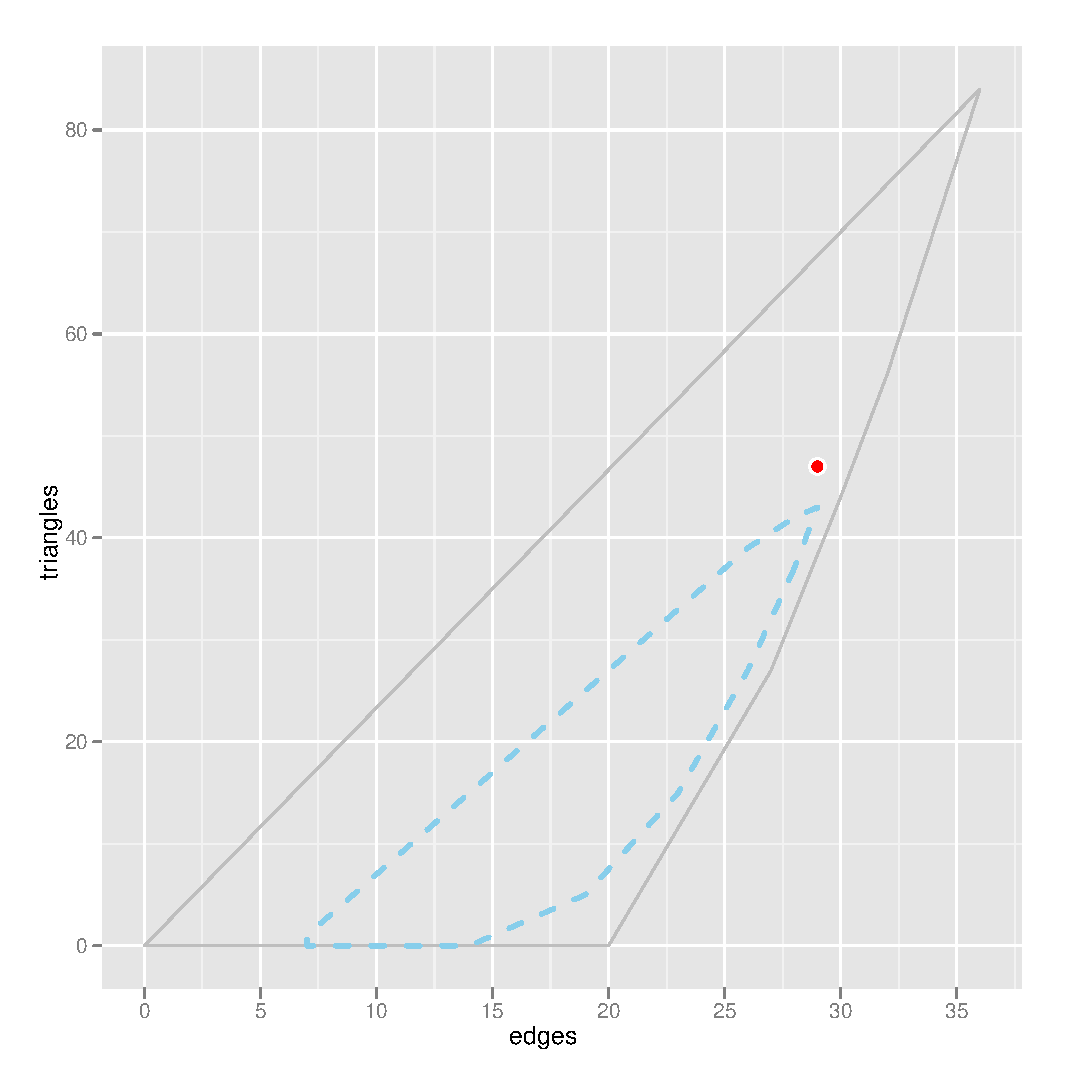
\includegraphics[height=2.8in,width=2.8in]{Figures/MCsample-far}
%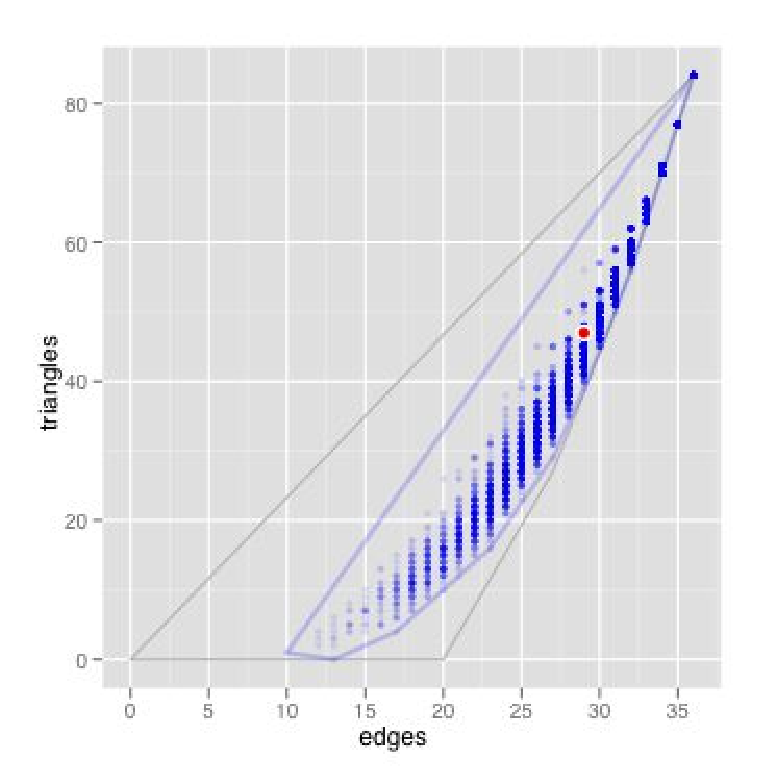
\includegraphics[height=2.8in,width=2.8in]{Figures/MCsample-MLE}
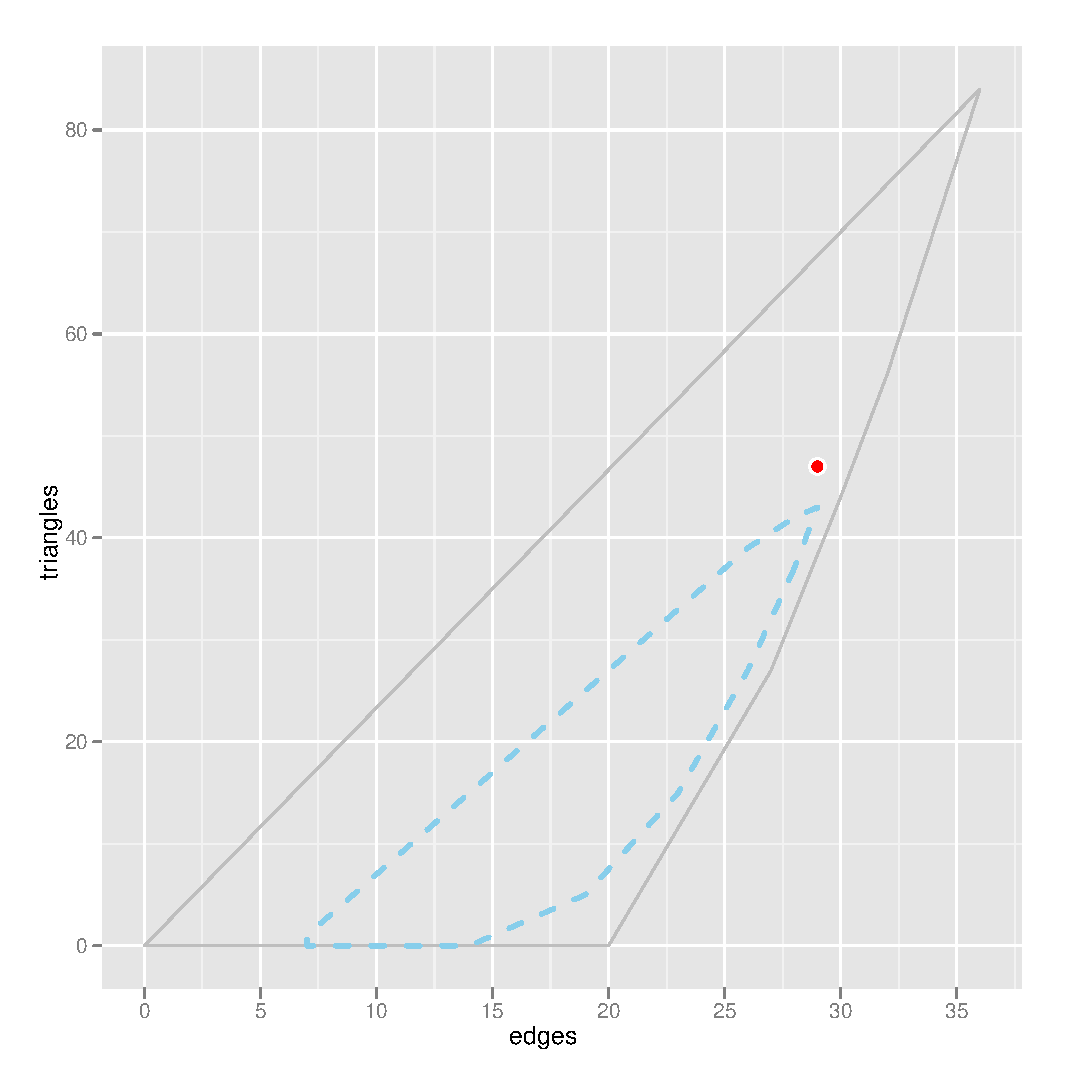
\includegraphics[width=3.4in]{Figures/MCsample-far}
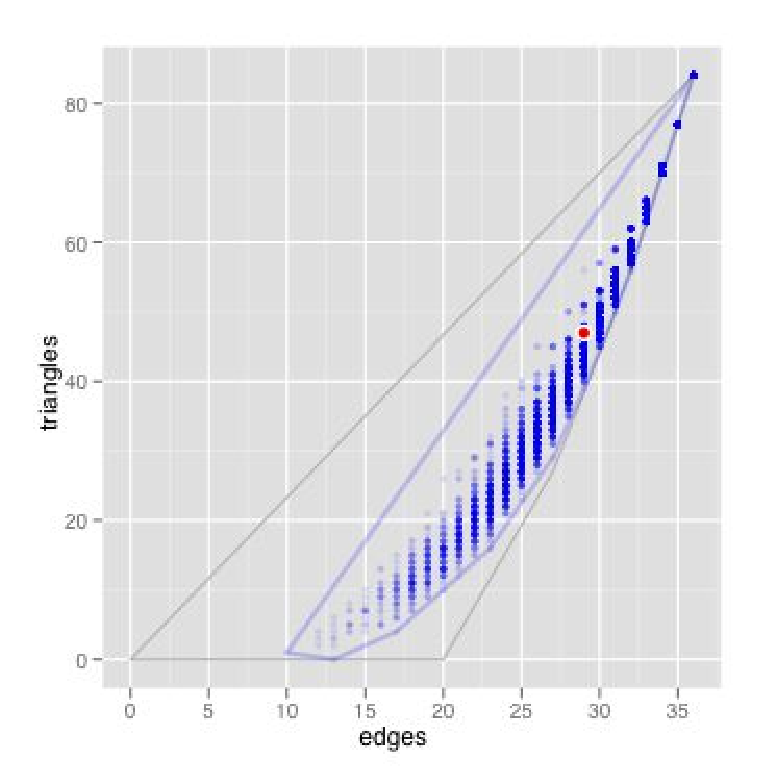
\includegraphics[width=3.4in]{Figures/MCsample-MLE}
\caption[Network statistics for 10,000 Monte Carlo samples when MLE exists]
{Network statistics for 10,000 Monte Carlo samples generated from models 
with $\eta= (0,0)$, top, and $\eta = \etaMLE = (-0.389, 0.418)$,
bottom.  The observed network statistic is $(29,47)$, depicted by the 
larger point.  When $\eta$ is the MLE, the observed statistic is 
the mean of the MC sample points generated. }
\label{F:MC cloud}
% (-0.3890151, 0.4177752) % from trust
\end{figure}
For this problem, the MLE for $\eta$ is found to be
\begin{align*}
\etaMLE = (-0.389, 0.418),
\end{align*}
which matches the results we get from applying \texttt{trust} to numerically
maximize the log likelihood function.

%%%%%%%%%%%%%%%%%%%%%%%%%%%%%%%%%%%%%%%%%%%%%%%%%%%%%
\subsection{Case: MLE does not exist; observed statistic on one-dimensional face}
Suppose the observed network has network has 31 edges and 50 triangles.  Then 
$g(\yobs) = (31,50)$ lies on the boundary of the convex support as depicted in 
Figure \ref{F:MC face}.  To be precise, the observed network statistic $(31,50)$ lies 
on the interior of a line segment on the boundary of the convex support with 
end points $(30,44)$ and $(32,56)$. 
By Theorem~\ref{Thm:MLE existence}, the MLE does not exist
in the conventional sense.

Our algorithm begins as before, generating MC sample point clouds 
from the distribution indexed by $\eta = (0,0)$.  Because the convex 
support is not assumed to be known, 
the algorithm cannot determine at the outset that the MLE does 
not exist; rather, it can only generate more sample point clouds as it climbs the log 
likelihood surface, with successive point clouds moving towards the observed statistic.
Eventually, the observed statistic will lie exactly on the boundary of a point cloud.
When this occurs, the algorithm must 
\begin{enumerate}
\item determine empirically the face $F$ in which the observed statistic lies in the 
relative interior of,
\item decide if $F$ is in fact the boundary of the convex support $C$.
\end{enumerate}  

The first task can be done using the linear programming methods 
described in Chapter~\ref{Chapter:Linear programming}.  
In particular, by use of the \texttt{linearity} function, we can identify the 
extreme points of the empirical face $F$.
 

The second task turns out to be more difficult.  
We first calculate an empirical GDOR by the methods in Section~\ref{S:GDOR calc}, which here give us
\begin{align*}
	\delta = (6,-1).
\end{align*}

If this $\delta$ is a GDOR and $g(\yobs) \in \rbd C$, then 
\begin{align} \label{E:Face check}
	\inner{w - g(\yobs), \delta=0}
\end{align}
for all $w \in F$.  
Thus \eqref{E:Face check} gives an easy way to check if 
any point is in the empirical face $F$.
We then assume that if a substantial portion of the sample points generated, say 
more than 60\%, land on this empirically determined face $F$, then it is in fact a boundary of 
the convex support $C$.  

In this example, the algorithm determines empirically that three points 
from the MC sample---$(30,44)$, $(31,50)$, and $(32,56)$---lie on a 
one-dimensional face, as depicted in Figure \ref{F:MC face}.  
If less than 60\% of the sample points land on this empirical face, the 
algorithm continues to sample, trying to get a sample point cloud even closer to the 
observed statistic.  We choose such a high proportion for a cutoff to eliminate---or 
at least, greatly reduce---the possibility of misidentifying a boundary.
(We deal later with a case where 100\% of the MC sample points form a face which is 
\emph{not} on the boundary of $C$.)  The empirical GDOR $\delta$ that we calculate 
can also be used as an effective search direction when it is not yet determined that 
$F$ is a boundary of $C$.  If $F$ is in fact a boundary of $C$, then 
by Theorem~\ref{Thm:LCM}, this threshold will be met.  A sample meeting this requirement 
is depicted in Figure~\ref{F:MC face}. 

\begin{figure}[h!]
\centering
%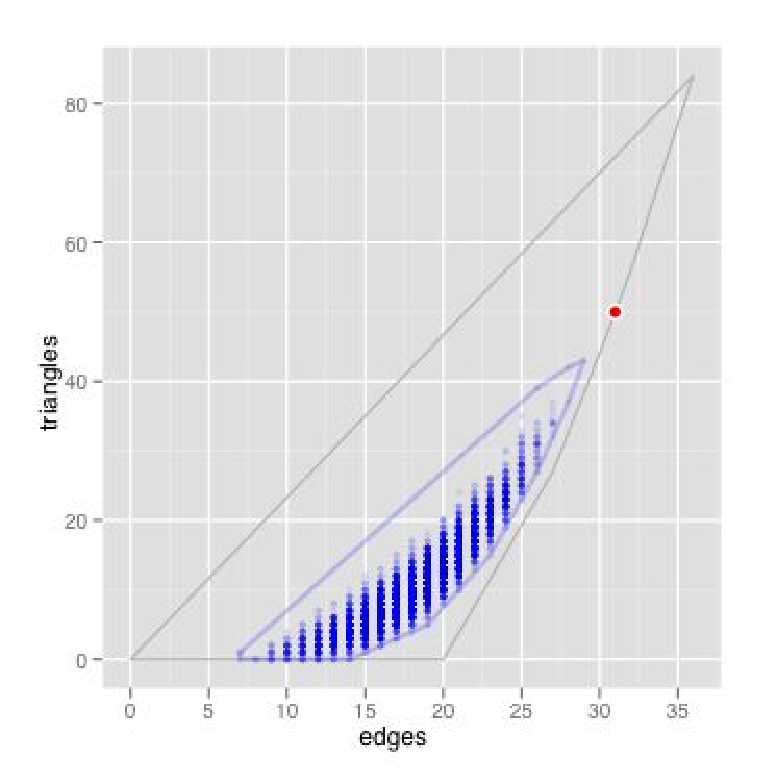
\includegraphics[height=2.7in,width=2.7in]{Figures/MCsample-boundary}
%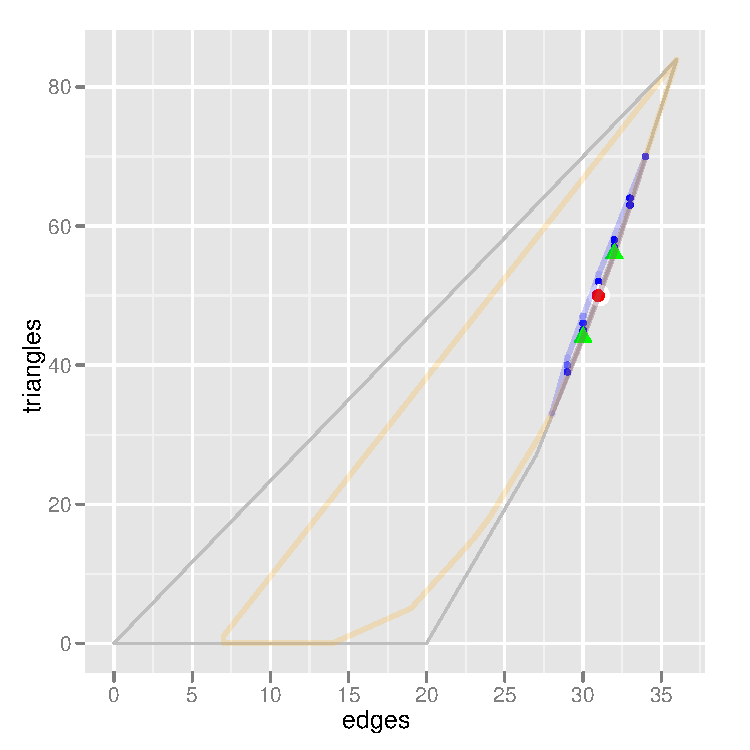
\includegraphics[height=2.7in,width=2.7in]{Figures/MCsample-77face}
%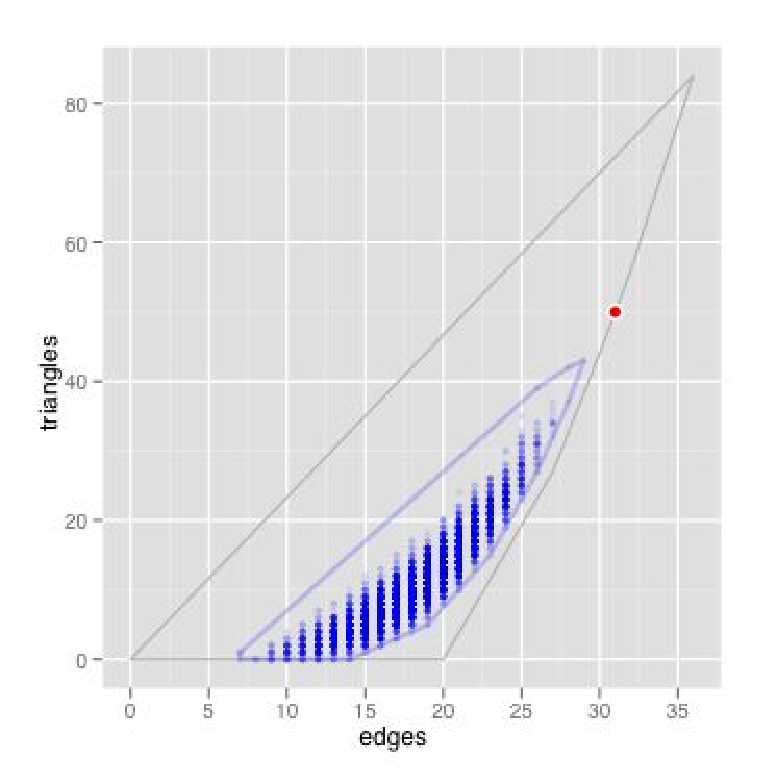
\includegraphics[width=3.5in]{Figures/MCsample-boundary}
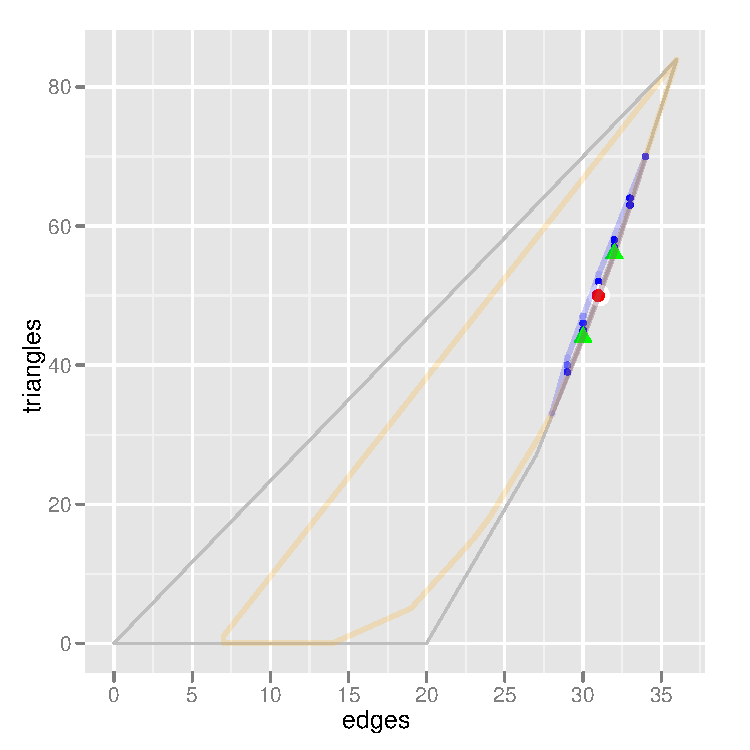
\includegraphics[width=5in]{Figures/MCsample-77face}
\caption[Network statistics for 10,000 Monte Carlo samples when MLE does not exist]
{Network statistics for 10,000 Monte Carlo samples when the MLE does not exist.  
The observed statistic, $(31,50)$, is the larger point on the boundary.
A face has been identified,
defined by $(30,44)$, $(31,50)$, and $(32,56)$ and marked 
by triangles (the triangle for 
$(31,50)$ is not visible since it is also the observed statistic).  
Here, 77\% of the MC sample points fall on these three points.
The lighter colored polytope is the convex hull of all previously 
sampled points.
}
\label{F:MC face}
\end{figure}

By identifying the empirical face $F$ in whose relative interior the observed 
statistic lies, 
the algorithm has not only concluded that the MLE does not exist in the conventional 
sense, it has also defined $F$ as the convex support for the new limiting conditional 
model for which the MLE must exist by Corollary~\ref{Cor:LCM MLE exists}.
The algorithm then maximizes this new exponential family using the same 
iterative approach as before.  The gradient of the LCM log likelihood is approximated 
using \eqref{E:nabla ell approx LCM},
\begin{align*}
	\nabla \ell( \eta )^{LCM} \approx g(\yobs) - \frac{1}{p} \sum_{i=1}^p g(Y_{(p)})
\end{align*}
where $g(Y_{(1)}), \ldots, g(Y_{(p)})$ is the subsample of the MC sample points 
restricted to the empirical face, $(30,44)$, $(31,50)$, and $(32,56)$ in this case.  
The maximizer $\etaLCM$ of this log likelihood is found to
be
\begin{align*}
\etaLCM = (126.8, -21.1).
%> theta.current
%    edges triangles 
%126.75482 -21.10183 
\end{align*}
The LCM, however, is not identifiable, since the support is now only one-dimensional 
compared to two in the original model.  That is, there must exist a constancy space 
of this new model, $\Gammalim$, such that 
\begin{align} \label{E:Gammalim}
\ell( \eta + \gamma )^{LCM} = \ell( \eta )^{LCM}
\end{align}
for any $\gamma \in \Gammalim$.  By Theorem~\ref{Thm:DOC}, the GDOR $\delta$ 
that the algorithm found is one such $\gamma$.
%By Corollary~\ref{Cor:strictly increasing}, a GDOR $\delta$ is a direction along which the log likelihood function is strictly increasing, and by 
%Theorem~\ref{Thm:LCM}, we know that
%\begin{align} \label{E:GDOR lim}
%	\lim_{s \to +\infty} \ell( \etaLCM + s \delta) = \sup_{\eta} \ell(\eta).
%\end{align}
%Then by \eqref{E:Gammalim} and \eqref{E:GDOR lim}, note that $\ell(\etaLCM + \gamma + 
%s \delta)$ goes off to $+\infty$ as $s$ increases.  

To construct one-sided 95\% confidence intervals, we need to find the value of 
$s$ for which the the distribution indexed by $\etaLCM + \gamma + s \delta$ 
assigns a probability of 0.05 to the event that a sample falls on the 
face of interest.  That is, find $s$ such that
\begin{align*}
P_{\etaLCM + \gamma + s \delta}(g(Y) \in F ) = 0.05.
\end{align*}
We can generate MC samples 
of $g(Y_1), \ldots, g(Y_m)$ from the distribution with parameter $\etaLCM + \gamma + s 
\delta$ and see for what value of $s$, 5\% of the sample lies in the 
empirical face we found.  Some numerical calculations show that the original
 exponential family indexed by $\eta = (9.145, -1.500)$ puts 5\% of
  the MC sample on this face.  
Expressing this as non-simultaneous 95\% confidence intervals, we get
\begin{align*}
	[9.145, +\infty)\\
	(-\infty, -1.500],
\end{align*}
where the direction of the interval for the second component is flipped because the 
second component of $\delta$ is negative.

We also applied a trust optimization routine on the original log 
likelihood in attempt to maximize it.  The maximum of course does not exist, but
because the surface flattens so much, the routine returns a value it perceives as a maximizer,  
\begin{align*}
 	\hat{\eta}_{\textrm{trust}} = (135.6, -22.6).
 \end{align*}
This value of $\eta$ is well within the confidence region and hence indexes a distribution
in the neighborhood of the LCM.
%Alternatively, in mean value parameterization, the
%non-simultaneous 95\% confidence intervals for the edge and triangle parameters are
%\begin{align*}
%	[29.7, 31]\\
%	[44.1, 50],
%\end{align*}
%where the upper bounds are the observed data and hence the MLE in this parameterization.
%%Incidentally, the mean parameterization of $\hat{\eta}_{\textrm{trust}}$ is $(31,50)$, 
To summarize, our algorithm realized correctly that the MLE for 
this model does not exist in the conventional sense.
The algorithm first identified a GDOR, $\delta = (6,-1)$, along which 
the log likelihood is strictly increasing.  It then used this GDOR to determine
a one-dimensional face $F$ in which the observed statistic lies 
in the relative interior.  The algorithm then found $\etaLCM$, the 
maximizer of the exponential family
which has $F$ as its convex support.  Finally, the algorithm used the
values of $\etaLCM$ and $\delta$ to calculate the end points for 
one-sided confidence intervals for the natural parameter.


%%%%%%%%%%%%%%%%%%%%%%%%%%%%%%%%%%%%%%%%%%%%%%%%%%%%%
\subsection{Case: MLE does not exist; observed statistic on zero-dimensional face}
If the observed network has statistic $g(\yobs) = (27, 27)$,  then 
$g(\yobs)$ is an extreme point
of the convex support $C$ (it is one of the six defining vertices of $C$, depicted by
a square point in Figure~\ref{F:g9-hull}).  In this case, the point is itself the 
face with zero-dimension and the MLE does not exist.  

The algorithm proceeds as before, and concludes that the 
point $(27,27)$ is the empirical face $F$ and lies on the boundary of $C$, using the
same 60\% criteria as before.
In this case, the limiting conditioning model is completely unidentifiable, and thus 
any value for $\eta$ will be a maximizer.  Our particular implementation found that
\begin{align*}
	\etaLCM = (30.0, -7.2 ).
\end{align*}
%29.96274 -7.216648
The normal cone to the observed statistic $N_C (g(\yobs) )$ in this case is a two-dimensional cone (and not a subspace), bounded by 
two directions,
\begin{align*}
	 \{ (3.857,   -1),	(5.667,   -1) \}.
\end{align*}
The linear programming routine in our algorithm found a GDOR of 
$\delta = (4.4, -1)$, clearly 
in the relative interior of this normal cone, which is itself not calculated by
our algorithm but done here for comparison purposes.
Proceeding as before, we find 95\% one-sided confidence intervals for $\eta$ of 
\begin{align*}
	[14.32, +\infty)\\
	(-\infty, -3.65],
\end{align*}

%The 95\% one-sided confidence intervals for mean parameterization is
%\begin{align*}
%%23.84996, 15.63127
%	[23.8, 27)\\
%	[15.6, 27].
%\end{align*}

For comparison, a trust optimization routine on the original log 
likelihood yielded a value it perceives as a maximizer,  
\begin{align*}
%  66.13789     -14.67444
 	\hat{\eta}_{\textrm{trust}} = (66.1, -14.7).
 \end{align*}

%%%%%%%%%%%%%%%%%%%%%%%%%%%%%%%%%%%%%%%%%%%%%%%%%%%%%
\subsection{Case: MLE exists but observed statistic is very near boundary} 
\label{S:Example:9node problematic point}
If the observed data has network statistic $(21, 4)$, it is in the relative interior of 
the convex support $C$ (see Figure~\ref{F:MC problem}) and so the MLE exists.
It lies very close to the boundary, however, and from a mean value parameter 
perspective, this observed statistic 
corresponds to a nearly degenerate distribution. The Shannon entropy function would show this 
point to have extremely small entropy, corresponding to a model that puts most of its 
probability on very few points \citep{Rinaldo:2009}.

The log likelihood for this model is extremely flat, causing some disagreement among 
numerical optimization routines for MLE estimates, though log likelihood values 
themselves are nearly identical.  Using a trust optimization routine we calculate that 
\begin{align*}
%$(24.44, ?6.65)$ from optim.
\etaMLE = (28.86, -7.76).
\end{align*}
The most problematic aspect of this model for us here, however, is that our algorithm 
may conclude---incorrectly---that the MLE does \emph{not} exist, 
and proceeds to 
calculate the MLE of an LCM as in the previous examples.  In this case, we used
an MC sample size of 10,000 (recall that we are using a perfect Monte Carlo sampler
from the exact distribution rather than an MCMC sampler).

How does this happen?  Does this make our algorithm not useful in practice?

Our algorithm begins in the same manner as described previously.  As the algorithm 
proceeds uphill on the log likelihood function, it eventually iterates $\eta_k$ to a 
value (for example, $(35.34, -9.56)$) where all 10,000 MC sample points generated 
from the model with this parameter value may fall on the six points on the line segment 
between $(20,0)$ and $(25,20)$, as depicted in Figure~\ref{F:MC problem}.  
The observed value $(21,4)$ is one of these six points, and the algorithm concludes
that it has found an empirical face on the boundary of $C$.

In order for the algorithm to have correctly concluded that $(21,4)$ was in the 
relative interior of $C$, the extreme point $(27,27)$ 
would need to have occurred in the MC sample
(as it occasionally did, in which case the algorithm found the MLE as usual).  
However, though this point is not far from the end point $(25,20)$ of our line
segment, the model indexed by the current parameter value 
assigns a probability of 0.000032 to this point.  In fact, even the 
MLE model only assigns a probability of 0.00045 to this point.  
So, the extreme point that is critical for fully determining the convex support 
is assigned very low probability and may not appear in a MC sample of 10,000.

\begin{figure}[h!]
\centering
%%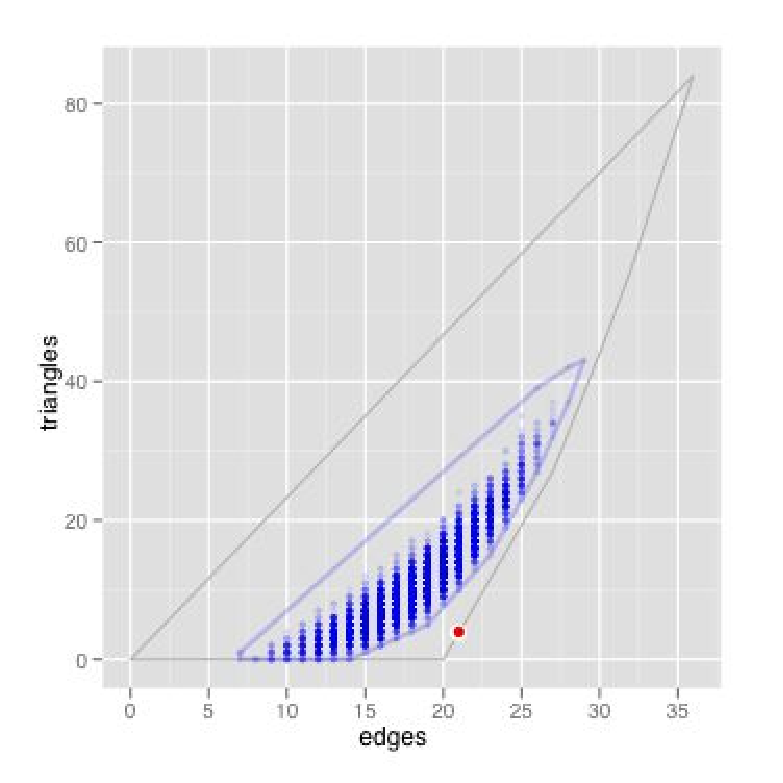
\includegraphics[height=2.4in,width=2.4in]{Figures/MCsample-problem}
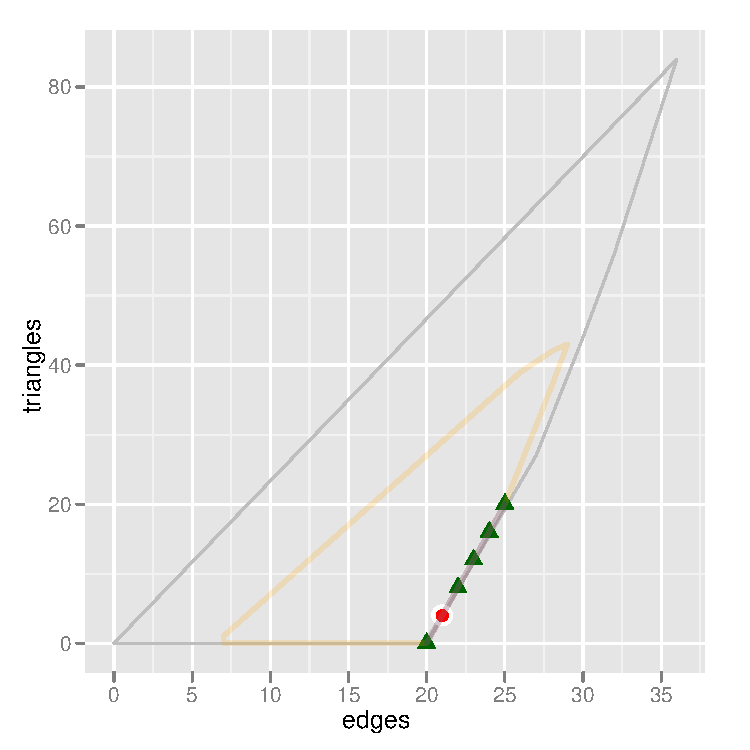
\includegraphics[width=5in]{Figures/MCsample-fakeface}
\caption[Network statistics for 10,000 Monte Carlo samples when the observed 
statistic is very close to a boundary]
{Network statistics for 10,000 Monte Carlo samples when the observed 
statistic is very close to a boundary.  The observed statistic is $(21,4)$.  Here, 
all 10,000 samples fall on six points (marked by triangles) on a line segment 
that appears to be on the boundary of the convex support.  However,
all points except $(20,0)$ are in the interior.  The absence of the 
extreme point $(27,27)$ in this sample---and all previous samples---leads
to this misidentification.
The lighter colored polytope is the convex hull of all previously 
sampled points.}
\label{F:MC problem}
\end{figure}

Thus in most cases, our algorithm treats the line segment as a boundary of the 
convex support in which the observed statistic lies in the relative interior, and 
hence the support of the LCM.  It proceeds as in the first
example finds the MLE of this LCM,
\begin{align*}
	\etaLCM = (35.38, -9.39),
\end{align*}
after which it then calculates one-sided confidence intervals for $\eta$.

On first glance this is very troubling: our algorithm arrives at the wrong conclusion 
about the existence of the MLE, and $(35.38, -9.39)$ does not look close 
to the true MLE of $(28.86, -7.76)$.  However, we believe the algorithm is
actually performing better than it might initially appear.
A step back should be taken and the goal of the analysis revisited.  

What is the purpose in finding the MLE?  In particular, what does one do with these values once they are found?

If the end goal is to try to interpret meaning out of these numbers by their sign and  
magnitude, then we indeed have a problem---our numbers are just wrong.  
However, if the MLE is viewed as an 
index to a specific model that assigns the highest probability to the observed data,
then we claim that the model we have found---the LCM with parameter value 
$\etaLCM$---is in fact remarkably similar to the original model indexed by the true MLE.  A 
reasonable metric for this comparison is a sum of the absolute difference in 
probabilities assigned to each point in the sample space,
\begin{align*}
	\sum_{y \in \YY} \abs{ P_{\etaMLE}(g(Y) =g(y) ) -  P_{\etaLCM}(g(Y) = g(y))  }.
\end{align*}
The probabilities assigned by each of these models to the six points on the 
empirically determined face is summarized in Table~\ref{T:LCMvsMLE}.

% latex table generated in R 2.11.1 by xtable 1.5-6 package
% Fri Sep 10 13:22:25 2010
\begin{table}[h!] 
\begin{center}
\caption[Comparison of probabilities assigned by LCM model and 
original MLE model to empirical face of 9-node network]
{Probabilities assigned by LCM model and original MLE model 
to points on empirical face of 9-node network.  The observed statistic is 
$(21,4)$.  For the MLE model, the probabilities do not sum to 1 since it assigns 
positive probability to points other than these six.}

\begin{tabular}{rrrrr}
\\  \hline
 & Edges & Triangles & LCM & MLE \\ 
  \hline
1 & 20 & 0 & 0.3414 & 0.3425 \\ 
  2 & 22 & 8 & 0.2019 & 0.2009 \\ 
  3 & 21 & 4 & 0.3914 & 0.3911 \\ 
  4 & 23 & 12 & 0.0566 & 0.0561 \\ 
  5 & 24 & 16 & 0.0081 & 0.0080 \\ 
  6 & 25 & 20 & 0.0005 & 0.0005 \\ 
   \hline
   &  &  & 1.0000 & 0.9990 \\ 
\end{tabular}\label{T:LCMvsMLE}
\end{center}
\end{table}

Here, the sum of the absolute value of differences on these empirical points is only 
$0.0031$.  Including the additional 0.001 of probability on points that are outside 
the LCM support, this total still only comes to $0.0041$, a difference that would seem 
insignificant for most applications.  

Of course, there are practical issues: even if a researcher is interested in the 
MLE distribution, she may want the software to simply 
return MLE values to keep around for later analysis.  Here, we are suggesting that the 
analysis return LCM MLE values and an LCM model (perhaps in the form of a GDOR or
convex support).  The researcher may understandably be confused, especially if she knew in 
advance that the MLE was guaranteed to exist.  
To make matters yet more confusing, it is possible that the
algorithm does produce the extreme point $(27,27)$ in a sample and finds the MLE
in the original model.  Thus by randomness the researcher might get either conclusion.
However, we emphasize again that
any probability calculations---and hence inference---would be nearly identical, though perhaps not ``out of the box".

It may be of interest to note that $\etaLCM$ and $\etaMLE$ index nearly identical 
models in the LCM, with the difference due almost entirely to the lack of 
identifiability of the LCM.  A GDOR to the (incorrect) empirical face is 
$\delta = (4,-1)$, which is also a direction of constancy for the LCM. 
%(that is, $\delta \in \Gammalim$).  
Then by \eqref{E:Gammalim}, 
\begin{align*}
	\ell(\etaLCM)^{LCM} &= \ell( \etaLCM + \gamma )^{LCM}\\
				 &= 	\ell(\etaLCM + k \, (4,-1))^{LCM}.
\end{align*}
If we had perfect knowledge and chose $k = -1.63$,
\begin{align*}
	\etaLCM  -1.63 \, (4,-1)= (28.86, -7.76) 
\end{align*}
matching the MLE to the significant figures considered.  Thus in this case, $\etaLCM$ 
and $\etaMLE$ index nearly identical models of the LCM.

If we allowed the algorithm to finish the incorrect analysis and computed 
one-sided 95\% confidence intervals for $\eta$, we get 
\begin{align*}
%14.495152 -3.703202 
	[20.46, +\infty)\\
	(-\infty, -4.85].
\end{align*}
As expected, $\etaMLE$ is well within these intervals.
%20.462923 -4.850603 

%\begin{align*}
%	\hat{\theta}_{MLE} &= (28.85685, -7.75672)\\
%	\hat{\theta}_{LCM} &= (35.3831787, -9.387266),
%\end{align*}

%Well, remember that for LCM's we are looking to construct one-sided CIs.  But here, 
%what happens if we go off to infinity in this supposed direction of recession?  The 
%log-likelihood will eventually dip back down!  So, we can constructed two-sided CI's, 
%I think.  But, my calculations got me something that seems pointlessly wide: 
%\begin{align*}
% (3.503179,  -1.417266 )\\
% (71.22318,  -18.34727 ).
%\end{align*}

%%%%%%%%%%%%%%%%%%%%%%%%%%%%%%%%%%%%%%%%%%%%%%%%%%%%%
%\subsection{Three-dimensional sufficient statistic}
%In order to increase the complexity of the problem yet still have the ``truth" for 
%comparison, we also considered 7-node graph with network statistics edges, two-stars, 
%and triangles, a classic model in the literature first suggested by \citet{Frank:
%1986}.  Since then it has been criticized for its problematic behavior by \citet
%[really? check this]{GOF}, precisely related to the issue of non-existence MLEs (or 
%degeneracy???).
%
%The algorithm proceeds in exactly the same way, the difference now being that the 
%empirical face may have as many as two dimensions instead of one.  This makes for a 
%more interesting variety of constancy spaces for the LCM.  We only consider cases here 
%that add a notably different flavor than the two-dimensional case.
%
%\subsubsection{Observed value, $y_{obs}$, is on two-dimensional face}
%\subsubsection{Observed value, $y_{obs}$, is on one-dimensional face}
%\subsubsection{MLE does not exist; observed statistic on two-dimensional face but not 
%fully discovered}
%
%Set $y_{obs} = (14, 8, 43).$
%This point is on the boundary, which is a 2-dim face.
%
%The MC sample, however, does not cover the entire face.  This is a new scenario, but 
%it should not be a problem.  Those points on the actual face that are not included are 
%simply points of low probability.
%
%Only issue outstanding with this is how long it takes to find the LCM MLE.  Having a 
%surprisingly hard time with this.  Question: is it doing any worse than when we 
%started with a 2-dim sample space?



\chapter{Discussion}
We have presented a simple line search algorithm for finding the MLE of a regular 
exponential family when the MLE 
exists.  The algorithm avoids the trial and error experimentation of tuning parameters 
and starting points commonly associated with optimization routines
not invented by optimization specialists.  Our algorithm is modeled after algorithms 
discussed in optimization textbooks \citep{Fletcher,NW,Sun:2006},
all of which are safeguarded to ensure rapid automatic convergence.
%Because it only relies on first order derivatives, this approach avoids problems with 
%near-singular Fisher information 
%matrices that plague methods like Newton-Raphson.  The reliant on a curvature 
%condition for step size makes it less 
%sensitive to poor initial values that are problematic for MCMC-MLE and  SA in 
practice.

Convergence is guaranteed when the gradient can be calculated exactly.  Even when the 
gradient cannot be calculated 
exactly and is only estimable via MCMC, the algorithm is still useful in practice, as 
demonstrated by the Ising model 
example.  We have also described a way to construct and use confidence intervals to 
make convergence highly probable.

The algorithm can be computationally demanding.  When the current iteration approaches 
the solution, the 
curvature condition for step size becomes more difficult to satisfy and the method may 
require several iterations of 
MCMC sampling and perhaps an increase in MCMC sample size.  Eventual increase in MCMC 
sample size is unavoidable,
because the achievable accuracy is inversely proportional to the square root of the 
MCMC sample size, as in all Monte Carlo.
Thus we believe the best use of this algorithm is in combination with other faster 
methods like MCMC-MLE \citep{Geyer:1992}
or Newton-Raphson safeguarded by our line search algorithm.  Our 
algorithm should be used from ``long range'', when one has no good intuition for an 
initial value and is concerned about 
picking one that is far from the MLE.  The switch between types of search direction 
(steepest ascent, conjugate gradient,
or Newton) within our algorithm or the switch to another algorithm (such as MCMC-MLE 
\citep{Geyer:1992})
need not require manual intervention.  When used in combination in this
manner, we do not think the confidence intervals are necessary as the curvature 
condition is quite easily satisfied 
when the current iteration is far from the MLE.

One way to improve performance is to use conjugate gradient search directions rather 
than steepest ascent.  In our 
examples, this reduced the number of iterations by over 25\%.  However, in other 
problems we tried with different 
dimensionality, this performance varied significantly and it appears that no guarantee 
can be made about quantity of 
improvement in performance, though in all cases we examined, it never did worse.  This 
is no surprise, because the
necessity of ``preconditioning'' for good performance of the conjugate gradient 
algorithm is well known (but no
good ``preconditioner'' is available for maximum likelihood in exponential families).

There are several outstanding issues.  Most notably, we have not showed convergence of 
the algorithm when the gradient 
is approximated via MCMC.  This is a more difficult theoretical problem and is the 
motivation for stochastic 
approximation research.  
Further work is necessary to determine if one can adapt our restrictive curvature 
condition \eqref{E:Wolfe-mod} to the 
approach of \citet{Andrieu:2005} or \citet{Liang:2010} in MCMC stochastic 
approximation.  

Another remaining issue is the stopping criteria: what value should be chosen for $
\epsilon$ in the exit condition
$\lVert  \nabla \ell( \eta_k ) \rVert < \epsilon$?  Because the value of $\lVert  
\nabla \ell( \eta_k ) \rVert$ can only 
be approximated via MCMC, one cannot be certain if this condition is actually 
satisfied.  Here again, the switch to 
another methodology may be appropriate, though at least in our Ising model example, 
our use of 10,000 for the MCMC 
sample size and 0.005 for $\epsilon$ were successful in obtaining a reasonable 
parameter estimate. 

 A final remaining issue is estimation of Monte Carlo error of the estimates.  Here 
too we recommend switching to another
algorithm at the end.  The MCMC-MLE procedure gives accurate error estimates \citep
{Geyer:1994}.
For very small steps these are essentially the same as the Monte Carlo error of a 
single unsafeguarded Newton-Raphson step,
so the method in \citep{Geyer:1994} can be used for either.

%A natural extension of this algorithm is to the case where the MLE may not exist.  
%This occurs with positive probability for discrete state space exponential families and 
%is a practical concern when estimating parameters \citep{Rinaldo:2009, Geyer:gdor}.  
%In such instances, the concave log likelihood continues to increase as $\eta \to \infty$ along 
%certain directions of recession.  Our algorithm can still be applied to such a setting to climb the 
%log likelihood until the gradient approaches zero and help identify the directions of recession. 




% References don't have to be double spaced either
\setstretch{1.3}
\bibliographystyle{ims}
%\bibliographystyle{imsart-nameyear}
\bibliography{References}
%\bibliography{/Users/saipuck/Tako/THESIS/References}


% text in appendices may be single spaced, if desired
\setstretch{1.3} % to 1.3 spacing
\appendix
\chapter{Proofs} \label{Section:Proofs}
%%Our algorithm minimizes the objective function $f$ by performing repeated one-
%dimensional updates.  
Before getting to the proof of this theorem, we need the 
following lemma to transfer global properties of the objective function to the 
objective function restricted to a 
search direction.

%%%%%%%%%%% BEGIN LEMMA %%%%%%%%%%%%%%
\begin{lemma} \label{Lemma:f min} 
Suppose a function $f:\RR^n \to \RR$ is proper, lower semicontinuous, and strictly 
convex.  Then the minimum for $f$ 
exists and is unique if and only if every nonempty level set $\lev_{\leq \alpha} f$ is 
bounded.
\end{lemma}

%%%%%%%%%%% PROOF - LEMMA %%%%%%%%%%%%%%

\begin{proof}[Proof of Lemma~\ref{Lemma:f min}]
Assume every non-empty level set is bounded.  Then by Theorem~1.9 in \citet
{Rockafellar}, the minimum of $f$ is finite 
and thus exists.  By strict convexity, this minimum is also unique.

Now assume the minimum for $f$ exists, denoted by $\min f$.  By assumption, the level 
set $\lev_{\leq \min f} f$ 
contains exactly one point.  By Corollary~8.7.1 in \citet{Rockafellar:1970}, the level 
sets $\lev_{\leq \alpha} f$ are 
bounded for every $\alpha$.  
\end{proof}



%%%%%%% WHERE OLD PROOF WAS.  REMOVED 3/5/11.




%\newpage
%\section{Proof of Exponential family log likelihood maximization}
\begin{proof}[Proof of Theorem~\ref{Thm:log like max}]
Let $f(\cdot)$ represent the negative log likelihood $- \ell(\cdot)$, the objective 
function to be minimized.  We proceed from the perspective of a minimization of a 
function $f(\cdot)$ since this is the convention in the optimization literature \citep
{NW,Rockafellar}.  %\citet{Okabayashi:longrange} prove a special case when the minimum exists, and this proof mimics that one with 

The negative log likelihood function $-\ell(\cdot)$ is strictly convex by 
\eqref{E:nabla2 ell}, and continuous since it is infinitely differentiable by 
\hl{LEHMAN} \citep{TPE2}.
It is bounded below by the negative LCM log likelihood as described by \eqref{E:LCM ll bound}.

The objective function $f$ is bounded below, strictly convex, and lower semicontinuous 
by assumption, and so by Lemma~\ref{Lemma:f min}, the global minimum exists.  
Then by Lemma~\ref{Lemma:f min}, all level sets of type $\lev_{\leq a} f$, $a \in \RR$ are bounded in $\RR^n$.  Restricting the set to be along a search 
direction $p_k$ maintains the 
boundedness of these sets.  By Lemma~\ref{Lemma:f min} again, the minimum in this 
restriction exists and is unique.     

Then, unless $\nabla f( x_k ) = 0$ in which case $x_k$ is already the solution, for 
each $k$, we can uniquely define $
\alpha_{c_k}$ and $\alpha_{min_k}$ as follows: 
\begin{align}
%	\theta_k &= \cos^{-1} \left( \frac{ -\nabla f_k^T p_k }{ ||\nabla f_k|| \, ||
%p_k||} \right) \label{E:cosine} \\
	\nabla f( x_k + \alpha_{c_k} p_k)^T p_k &= c \nabla f(x_k)^T p_k \label{E:alphac} 
\\
	\nabla f( x_k + \alpha_{min_k} p_k)^T p_k &= 0. \label{E:alphamin} 
\end{align}
The point $\alpha_{c_k}$ is uniquely defined because it is the minimizer of $\alpha 
\mapsto f( x_k + \alpha p_k) - 
\alpha c \nabla f( x_k )^T p_k$.
These values appear on the $\alpha$-axis in Figure \ref{F:Wolfe-mod}.
%%%%%%%%%%% FIGURE %%%%%%%%%%%%%%
\begin{figure}
\centering
\scalebox{.4}{\input{Figures/Wolfe-mod.pdf_t}}
\caption{Acceptable region for $\alpha$ according to curvature condition 
\eqref{E:Wolfe-ll} along direction $p_k$.}
\label{F:Wolfe-mod}
\end{figure}

%These values are illustrated on the $\alpha$-axis in Figure \ref{F:Wolfe-mod}.  
%Equation \eqref{E:alphamin} defines $\alpha_{min_k}$ to be the step size that would 
%make the 
%gradient at $x_{k+1}$ equal to zero and hence minimizes $f(x_{k+1})$, equation \eqref
%{E:alphac} 
%defines \alpha_{c_k} to be the step size that would make the gradient at $x_{k+1}$ 
%equal to 

By the strict convexity of $f$ and Theorem~2.14 in \citet{Rockafellar}, 
\begin{align}
	f( x_k + \alpha_{c_k} p_k ) &< f(x_k) +  \bigl[ \nabla f(x_k + \alpha_{c_k} p_k) 
\bigr]^T \alpha_{c_k} p_k. \notag 
\\
	\intertext{Applying \eqref{E:alphac} to the right hand side of the above gives}
	f( x_k + \alpha_{c_k} p_k ) &< f(x_k) + \alpha_{c_k} c \nabla f(x_k)^T p_k. 
	\label{E:b-less-a}
	\end{align}	
(See points $a$ and $b$ in Figure \ref{F:Wolfe-mod}).

The subproblem $\alpha \mapsto f(x_k + \alpha p_k)$ is strictly convex and hence 
monotonically decreasing at $\alpha_k$ 
such that $\alpha_{c_k} \leq \alpha_k \leq \alpha_{min_k}$ (in Figure \ref{F:Wolfe-mod}, see points $b$ and $c$).  That is,
\begin{align}
	f( x_k + \alpha_{min}p_k) &\leq f( x_k + \alpha_k p_k) \leq f( x_k + \alpha_{c_k} p_k). \label{E:f-sandwich}
\end{align}
	
Combining the second inequality of \eqref{E:f-sandwich} with \eqref{E:b-less-a}, we 
have	
\begin{align}
	f( x_k + \alpha_k p_k ) &< f(x_k) + \alpha_{c_k} c \nabla f(x_k)^T p_k,  
	\label{E:decrease}
	\intertext{which can be rearranged as}
	f(x_k)-f( x_k + \alpha_k p_k ) &>  -\alpha_{c_k} c \nabla f(x_k)^T p_k. 
	\label{E:f-lb}
\end{align}
This last inequality \eqref{E:f-lb} expresses a lower bound for the amount of decrease 
in our objective function at 
each step (the right-hand side is positive since $\nabla f(x_k)^T p_k < 0$ by 
assumption that $p_k$ is a descent 
direction).  It is this lower bound that we will use to cover the distance to the 
minimum of the objective function.  

We now turn our attention to \eqref{E:alphac}.  Define $x_{c_k} = x_k + \alpha_{c_k} p_k$.  Then
\begin{align}
	\nabla f( x_{c_k} )^T p_k &= c \nabla f(x_k)^T p_k. \notag
\end{align}
Subtracting $\nabla f(x_k)^T p_k$ from both sides gives
\begin{align}
	\left( \nabla f( {x_{c_k}} ) - \nabla f(x_k) \right )^T p_k &= ( c - 1 ) 
	\nabla f(x_k)^T p_k.  \label{E:c-1}
\end{align}

%\textbf{NEW: SAI 1/17/11}\\
\textbf{
By \eqref{E:nabla2 ell}, $\nabla^2 \ell(\eta)$ is bounded for finite state space $g(\YY)$, which is true by assumption.  Thus $| \nabla^2 f(x) | \leq K$ for some 
constant K for all $x$. 
Then by Theorems 9.2 and 9.7 in \citet{Rockafellar}, 
%since $\nabla^2 f(x)$ is assumed to be finite, 
$\nabla f(x)$ is Lipschitz continuous relative to the convex set $\RR^n$.}

%By Corollary~25.5.1 in \citet{Rockafellar:1970}, since $f$ is convex and 
%differentiable on the open convex set $\NN$, 
%it is actually continuously differentiable on $\NN$.  It is then Lipschitz 
%continuously differentiable relative to any 
%compact subset of $\NN$. 

Applying this to the compact level set $\lev_{\leq f(x_k)} f$, 
%which is contained in $\NN$ by assumption, 
there exists a constant $L < \infty$ such that
	\begin{align}
		|| \nabla f(x) - \nabla f(\tilde{x}) || \leq L || x - \tilde{x} || \quad \text
{for all $x, \tilde{x} \in \lev_
{\leq f(x_0)} f$}. \label{E:Lipschitz}
	\end{align} 

Applying \eqref{E:Lipschitz} to $x_{c_k}$ and $x_k$, we have
\begin{align}
|| \nabla f(x_{c_k}) - \nabla f(x_k) || &\leq L || x_{c_k} - x_k || \notag
\intertext{or}
|| \nabla f(x_{c_k}) - \nabla f(x_k) || &\leq L || \alpha_{c_k} p_k ||. \notag	
\end{align}

Multiplying both sides by $\lVert p_k \rVert$ gives
\begin{align}
	|| \nabla f(x_{c_k}) - \nabla f(x_k) || \cdot ||p_k || &\leq \alpha_{c_k} L || p_k ||^2 
	\notag \\
\intertext{and by Cauchy-Schwarz this implies}
	( \nabla f(x_{c_k}) - \nabla f(x_k) )^T p_k & \leq || 
	\nabla f(x_{c_k}) - \nabla f(x_k) || \cdot ||p_k || \label{E:from-Lipschitz} \\ 
	&\leq \alpha_{c_k} L || p_k ||^2. \notag
\end{align}
Substituting \eqref{E:c-1} into the left-hand side of this last inequality 
\eqref{E:from-Lipschitz} gives
\begin{align}
( c - 1 ) \nabla f(x_k)^T p_k &\leq \alpha_{c_k} L || p_k ||^2 \notag\\
\intertext{or}
-\alpha_{c_k} &\leq \frac{( 1 - c )}{L} \frac{ \nabla f(x_k)^T p_k}{ || p_k ||^2}. 
\label{E:-alpha}
\end{align}

%%%%%%
%%%%%%
Write out the first $k+1$ inequalities of \eqref{E:f-lb}:
\begin{align}
\begin{split}
	f( x_1 ) &< f(x_0) + \alpha_{c_0} c \nabla f(x_0)^T p_0 \\
	f( x_2 ) &< f(x_1) + \alpha_{c_1} c \nabla f(x_1)^T p_1  \\
	\ldots  \\
	f( x_{k} ) &< f(x_{k-1}) + \alpha_{c_{k-1}} c \nabla f(x_{k-1})^T p_{k-1}  \\
	f( x_{k+1} ) &< f(x_k) + \alpha_{c_k} c \nabla f(x_k)^T p_k 
\end{split}
	\label{E:to telescope}
\end{align}
Telescoping the right-hand side of \eqref{E:to telescope},
\begin{align*}
	f( x_{k+1} ) &< f(x_0) + c \sum_{j=0}^{k} \alpha_{c_j} \nabla f(x_j)^T p_j. \notag
\end{align*}
Noting that $\nabla f(x_j)^T p_j < 0$, we can substitute our upper bound 
\eqref{E:-alpha} for $-\alpha_{c_j}$ in the right-hand side above,
\begin{align}
	f( x_{k+1} ) &< f(x_0) - c \sum_{j=0}^{k} \frac{( 1 - c )}{L} 
	\frac{\nabla f(x_j)^T p_j}{ || p_j ||^2 } \nabla f(x_j)^T p_j \notag \\
	\intertext{which simplies to}
	f( x_{k+1} ) &< f(x_0) - c \sum_{j=0}^{k} \frac{( 1 - c )}{L} 
	\frac{ (\nabla f(x_j)^T p_j)^2}{ || p_j ||^2 }. 
\notag
\end{align}

Because $f(x)$ is bounded below by assumption, there exists some $M < \infty$ such 
that $f(x_0) - f(x_{k+1}) < M$ for 
all $k$. Then rearranging the above yields,

\begin{align*}
	\frac{c( 1 - c )}{L} \sum_{j=0}^{k}   
	\frac{ ( \nabla f(x_j)^T p_j )^2}{ || p_j ||^2 } &< M < \infty.
 \end{align*}
The angle $\theta_j$ between the search direction $p_k$ and steepest descent direction 
$-\nabla f_k$ can be expressed 
by $\cos \theta_j = \frac{ -\nabla f(x_j)^T p_j}{||\nabla f_j|| \cdot || p_j||}$.  
Substituting this into the equation 
above and taking $k \to \infty$,
\begin{align*}
	\frac{c( 1 - c )}{L} \sum_{j=0}^{\infty}  \cos^2 \theta_j ||\nabla f(x_j)||^2 &< \infty.
\end{align*}
Since $0 < c < 1$,
\begin{align}
	\sum_{j=0}^{\infty}  \cos^2 \theta_j ||\nabla f(x_j)||^2 &< \infty. \label{E:Z's}
\end{align}

The convergent series in \eqref{E:Z's} implies that 
\begin{align*}
	\cos^2 \theta_k || \nabla f(x_k) ||^2 &\to 0 \text{ as } k \to \infty.
\end{align*}
With the additional restriction on the search direction $p_k$ such that $\cos \theta_k 
\geq \delta > 0$ for some choice 
of $\delta$, for all choices of $k$, we get the desired convergence result of
\begin{align*}
	\lim_{k \to \infty} || \nabla f(x_k) || &= 0.
\end{align*}

\end{proof}


%%%%%%%%%%% BEGIN PROOF - Line Search Works  %%%%%%%%%%%%%%
Theorem 3.1 shows that the gradient of the objective function converges to 0.  The 
proof for Theorem 3.2 is concerned 
with the conditions for mapping this convergence to the convergence of the iterated 
parameter estimates $\eta_k$ to the 
unique MLE.  In particular, the mapping from $\eta_k$ to the gradient must be globally 
invertible.

\begin{proof}[Proof of Theorem~\ref{Thm:Line Search works}]

The Fisher information for a regular exponential family is non-singular by \eqref
{E:FI} and thus invertible.  If we 
consider the map defined by
\begin{align*}
	h(\eta) = \nabla c(\eta)
\end{align*}
where $c(\eta) = \log \kappa(\eta)$ is the cumulant function introduced in Section~\ref{S:ERGM setup}, its first derivative matrix is
\begin{align}
	\nabla h(\eta) = \nabla^2 c(\eta) = I(\eta) \label{E:nabla h eta}
\end{align}
which is again non-singular.  Since this is true for any $\eta$, by the inverse 
function theorem, $h$ is everywhere 
locally invertible.

In fact, $h$ is globally invertible. For any $\mu$ in the range of $h$, consider the 
function
\begin{align*}
	q(\eta) = \mu^T\eta - c(\eta).
\end{align*}
Since $\nabla^2 q(\eta) = - I(\eta)$ by \eqref{E:nabla h eta}, $q$ is strictly 
concave.  Therefore, a maximizer for $q$, call it $\hat{\eta}$, is unique if it exists and satisfies the first-order condition
\begin{align*}
	\nabla q( \hat{\eta} ) = 0.
\end{align*}
This in turn implies that
\begin{align*}
	\mu - h(\hat{\eta}) = 0
\end{align*} 
or
\begin{align*}
	\mu = h( \hat{\eta} ). \label{E:eta hat}
\end{align*}
Because of the assumption that $\mu$ is in the range of $h$, this means that 
$\hat{\eta}$ in fact exists, and by the 
strict concavity of $q$, is unique.  This implies that $h$ must be one-to-one and 
hence globally invertible.


Since $c$ is infinitely differentiable by Theorem~2.7.1 in \citet{TSH}, so is $h$, and 
by the inverse function theorem, 
so is $h^{-1}$ (even if we do not know the form of $h^{-1}$).  The first derivative of 
$h^{-1}$ can be expressed as
\begin{align*}
	\nabla h^{-1}(\mu) = \left [ \nabla h(\eta) \right ]^{-1} = \left [ I(\eta) 
\right ]^{-1}
\end{align*}
when $\mu = h(\eta)$ and is thus non-singular everywhere, including at the MLE of 
$\eta$, $\etaMLE$.

Thus our algorithm, which concludes that $ || \nabla \ell( \eta_k) ||  = || g(y) - h
(\eta_k) || \to 0$, implies that 
\begin{align*}
	\mu_k = h(\eta_k) \to g(y), 
\end{align*}
or
\begin{align*}
	h^{-1}(\mu_k)  \to h^{-1}\left (g(y) \right),
\end{align*}
or
\begin{align*}
	\eta_k  \to  \etaMLE.
\end{align*}

\end{proof}
%%%%%%%%%%% END PROOF %%%%%%%%%%%%%%

%\chapter{Proofs of Chapter \ref{sec:gibbs} Results}\label{sec:app1}
%\input{GibbsProofs}
%
%\chapter{Proofs of Chapter \ref{sec:examples} Results}\label{sec:app2}
%\input{ExampleProofs}




\end{document}